
\documentclass[11pt, a4paper]{book}
\usepackage{svn-multi}
\svnid{$Id$}
\usepackage{prelim2e}
\renewcommand{\PrelimWords}{Draft Copy \svnkw{Id}}
%%\newcommand*{\mysvnrev}{\svnrev}
\usepackage[hyperindex=true,
			bookmarks=true,
            pdftitle={}, pdfauthor={Xi Yang},
            colorlinks=false,
            pdfborder=0,
            pagebackref=false,
            citecolor=blue,
            plainpages=false,
            pdfpagelabels,
            pagebackref=true,
            hyperfootnotes=false]{hyperref}
\usepackage[all]{hypcap}
\usepackage[palatino]{anuthesis}
\usepackage{afterpage}
\usepackage{graphicx}
\usepackage{thesis}
\usepackage[square]{natbib}
\usepackage[normalem]{ulem}
\usepackage[table]{xcolor}
\usepackage{makeidx}
\usepackage{cleveref}
%\usepackage[centerlast]{caption2}
\usepackage{float}
\urlstyle{sf}
\renewcommand{\sfdefault}{uop}
\usepackage[T1]{fontenc}
\usepackage[scaled]{beramono}

\usepackage{multirow}

\usepackage[section]{placeins}



\renewcommand*{\backref}[1]{}
\renewcommand*{\backrefalt}[4]{
  \ifcase #1 %
    %
  \or
    (cited on page #2)%
  \else
    (cited on pages #2)%
  \fi
}




%      $Id: macros.tex 506 2009-10-05 16:57:07Z daniel $    

\usepackage{booktabs}
\usepackage{relsize}
\usepackage{xspace}
\usepackage{subfigure}
\usepackage{listings}
\lstloadlanguages{java}
\DeclareGraphicsRule{*}{pdf}{*}{}
\newcommand{\otoprule}{\midrule[\heavyrulewidth]}
\newcommand{\pldi}{ACM Programming Language Design and Implementation (PLDI)}
\newcommand{\taco}{ACM Transactions on Architecture and Code Optimization (TACO)}
\newcommand{\lctes}{ACM Languages, Compiler, and Tool Support for Embedded Systems (LCTES)}
\newcommand{\popl}{ACM Principles of Programming Languages (POPL)}
\newcommand{\ecoop}{European Conference for Object-Oriented Programming (ECOOP)}
\newcommand{\asplos}{ACM Architectural Support for Programming Languages and Operating Systems (ASPLOS)}
\newcommand{\sigmetrics}{ACM Measurement and Modeling of Computer Systems (SIGMETRICS)}
\newcommand{\oopsla}{ACM Object-Oriented Programming, Systems, Languages, and Applications (OOPSLA)}
\newcommand{\ismm}{International Symposium on Memory Management (ISMM)}
\newcommand{\veee}{ACM/USENIX Virtual Execution Environments (VEE)}
\newcommand{\micro}{ACM/IEEE International Symposium on Microarchitecture}
\newcommand{\isca}{ACM/IEEE International Symposium on Computer Architecture (ISCA)}
\newcommand{\icse}{International Conference  on Software Engineering (ICSE)}
\newcommand{\pact}{Parallel Architectures and Compilation Techniques (PACT)}
\newcommand{\casess}{ACM Compilers, Architectures, and Synthesis for Embedded Systems (CASES)}

\definecolor{tableheadcolor}{rgb}{0.8,0.8,1.0}
%\definecolor{tablealtcolor}{rgb}{0.9,0.9,1.0}
\definecolor{tablealtcolor}{rgb}{0.9,0.9,0.95}


\definecolor{todocolor}{rgb}{0.8,0.8,1.0}
\definecolor{fixcolor}{rgb}{1,0.8,0.8}
\definecolor{commentcolor}{rgb}{0.8,1.0,0.8}


\newcommand{\listingfigure}[3]{
\begin{figure}[ht!]
  \begin{center}
    \begin{minipage}[t]{\textwidth-4cm}
      \lstinputlisting{#1}
    \end{minipage}
  \end{center}
  \caption{#3}#2
\end{figure}}

\newcommand{\includeabchart}[5]{
\begin{figure}[ht!]
\begin{center}
\newcommand{\atitle}{#4}
\newcommand{\btitle}{#5}
\input{charts/#1.tex}
\end{center}
\caption{#3}#2
\end{figure}}

\newcommand{\placeholderfigure}[2]{
\begin{figure}[ht!]
  \begin{center}
    \resizebox{\textwidth-2cm}{0.7\textwidth-1.4cm}{todo}
  \end{center}
  \caption{#2}#1
\end{figure}}

\newcommand{\singlegraphfigure}[3]{
\begin{figure}[ht!]
  \begin{center}
    \includegraphics[width=\textwidth-2cm]{#1}
  \end{center}
  \caption{#3}#2
\end{figure}}

\usepackage[color=todocolor, colorinlistoftodos]{todonotes}

%\newcommand{\notinpart}{%
% \def\toclevel@chapter{-1}\def\toclevel@section{0}\def\toclevel@subsection{1}} \newcommand{\inpart}{
% \def\toclevel@chapter{0}\def\toclevel@section{1}\def\toclevel@subsection{2}}


%
% Stuff for pretty printing the source code using listings.sty
%


%% set Java as the default language
\lstset{
  numbers=left,
  numberstyle=\tiny,
  stepnumber=1,
  numbersep=2em,
  language=java,                         % the language
  basicstyle=\footnotesize\ttfamily,     % the basic font family to use
  commentstyle=\itshape,                 % the font for comments
  stringstyle=\ttfamily,
%  morekeywords={@Intrinsic, @Unboxed, @RawStorage}
}
%\lstset{language=java}

\newcommand{\textjava}[1]{{\lstset{basicstyle=\ttfamily}\lstinline@#1@}}
\newcommand{\textjavafn}[1]{{\lstset{basicstyle=\footnotesize\ttfamily}\lstinline@#1@}}
%\usepackage{lstasm}
\usepackage{setspace}
\usepackage{ifthen}
%\usepackage{color}
%\usepackage{smallheadings}

\long\def\sfootnote[#1]#2{\begingroup%
\def\thefootnote{\fnsymbol{footnote}}\footnote[#1]{#2}\endgroup}
%
% code
%

\newcommand{\address}{\textjava{Address}\xspace}
\newcommand{\ubregion}{\textjava{unbump-region()}\xspace}
\newcommand{\word}{\textjava{Word}\xspace}
\newcommand{\freeme}{\textjava{free()}\xspace}
\newcommand{\freemeunbump}{\textjava{unbump()}\xspace}
\newcommand{\freemeunbumpregion}{\textjava{unbump-region()}\xspace}
\newcommand{\freemeunreserve}{\textjava{unreserve()}\xspace}

%
% abbreviations
%


\newcommand{\eg}{e.g., }
\newcommand{\ie}{i.e., }

\newcommand{\GenMS}{\emph{GenMS}\xspace}
\newcommand{\GenImmix}{\emph{GenIX}\xspace}
\newcommand{\mmtk}{MMTk\xspace}
\newcommand{\jikes}{Jikes RVM\xspace} 
\newcommand{\jikesrvm}{\jikes} 
\newcommand{\jala}{Jalape\~{n}o\xspace} 
\newcommand{\jalapeno}{Jalape\~{n}o\xspace} 

\newcommand{\dacapo}{\textsf{DaCapo}\xspace}
\newcommand{\specjvm}{\textsf{SPECjvm98}\xspace}
\newcommand{\cattrack}{\textsf{cattrack}\xspace}
\newcommand{\spec}{\textsf{SPEC}\xspace}

\newcommand{\nurserytype}[1]{{\fontfamily{cmss}\selectfont \textsl{#1}}}
\newcommand{\alloc}{\nurserytype{allocate}\xspace}
\newcommand{\collect}{\nurserytype{collect}\xspace}
\newcommand{\redirect}{\nurserytype{redirect}\xspace}

\newcommand{\bmtype}[1]{{\textsf{#1}}}

\newcommand{\jbb}{\bmtype{jbb2000}\xspace}
\newcommand{\psjbb}{\bmtype{pjbb2005}\xspace}
\newcommand{\pjbb}{\bmtype{pjbb2005}\xspace}
\newcommand{\specjbb}{\bmtype{SPECjbb2005}\xspace}
\newcommand{\jess}{\bmtype{jess}\xspace}
\newcommand{\raytrace}{\bmtype{raytrace}\xspace}
\newcommand{\db}{\bmtype{db}\xspace}
\newcommand{\javac}{\bmtype{javac}\xspace}
\newcommand{\jack}{\bmtype{jack}\xspace}
\newcommand{\compress}{\bmtype{compress}\xspace}
\newcommand{\mpegaudio}{\bmtype{mpegaudio}\xspace}
\newcommand{\mtrt}{\bmtype{mtrt}\xspace}
\newcommand{\antlr}{\bmtype{antlr}\xspace}
\newcommand{\bloat}{\bmtype{bloat}\xspace}
\newcommand{\chart}{\bmtype{chart}\xspace}
\newcommand{\eclipse}{\bmtype{eclipse}\xspace}
\newcommand{\fop}{\bmtype{fop}\xspace}
\newcommand{\hsqldb}{\bmtype{hsqldb}\xspace}
\newcommand{\jython}{\bmtype{jython}\xspace}
\newcommand{\luindex}{\bmtype{luindex}\xspace}
\newcommand{\lusearch}{\bmtype{lusearch}\xspace}
\newcommand{\Lusearch}{\bmtype{Lusearch}\xspace}
\newcommand{\pmd}{\bmtype{pmd}\xspace}
\newcommand{\ps}{\bmtype{ps}\xspace}
\newcommand{\SPECjbb}{\bmtype{SPECjbb}\xspace}
\newcommand{\xalan}{\bmtype{xalan}\xspace}
\newcommand{\sunflow}{\bmtype{sunflow}\xspace}
\newcommand{\Sunflow}{\bmtype{Sunflow}\xspace}
\newcommand{\avrora}{\bmtype{avrora}\xspace}
\newcommand{\core}{Core2 Quad\xspace}
\newcommand{\corelong}{Intel Core2 Quad Q6600\xspace}
\newcommand{\phenom}{Phenom II\xspace}
\newcommand{\phenomlong}{AMD Phenom II X6 1055T\xspace}
\newcommand{\sandy}{i7-2600\xspace}
\newcommand{\sandylong}{Intel Core i7-2600\xspace}



\newcommand{\ghostscript}{\bmtype{ghostscript}\xspace}

\newcommand{\doi}[1]{\href{http://dx.doi.org/#1}{\nolinkurl{doi:#1}}}
%
% misc
%
\newcommand{\fix}[1]{\todo[color=fixcolor]{#1}}
\newcommand{\comment}[1]{\todo[color=commentcolor]{#1}}
\newcommand{\ifix}[1]{\todo[inline,color=fixcolor]{#1}}
\newcommand{\icomment}[1]{\todo[inline,color=commentcolor]{#1}}
\newcommand{\itodo}[1]{\todo[inline]{#1}}
\newcommand{\ignore}[1]{}
\newcommand{\mccenter}[1]{\multicolumn{1}{c|}{#1}}

%
% figure spacing
%
%\clubpenalty 10000
%\widowpenalty 10000
%\def\topfraction{0.9}
%\def\bottomfraction{0.9}
%\def\textfraction{0.1}
%\renewcommand{\singlespacing}{\renewcommand{\baselinestretch}{1.00}\small\normalsize}
%\renewcommand{\doublespacing}{\renewcommand{\baselinestretch}{1.5}\small\normalsize}
%\newcommand{\tight}{\renewcommand{\baselinestretch}{1.28}\small\normalsize}
%\renewcommand{\subfigbottomskip}{0.25ex}
%\renewcommand{\subfigcapskip}{0ex}
%\renewcommand{\subfigcapskip}{-1ex}
%\newcommand{\subfigshrink}{-0.75ex}
%\newcommand{\subfigcapspace}{2ex}

%\newcommand{\subwidth}[0]{.32\textwidth}


%
% margins
%
%\topmargin -.5truein
%\textheight 9truein
%\oddsidemargin .25truein
%\evensidemargin .25truein
%\textwidth 6truein


%
% crossreferencing footnotes
%
%\newcommand{\fnref}[1]{~(\ref{#1})}
%\newcommand{\onecolparbox}{3.1in}


%\newcommand{\textjava}[1]{{\lstset{language=java,basicstyle=\footnotesize\ttfamily}\lstinline@#1@}}
%\newcommand{\textasm}[1]{{\lstset{language=asm,basicstyle=\footnotesize\ttfamily}\lstinline@#1@}}

%%
%% Change the sections etc.
%%
%\makeatletter
%\parskip=0pt
%\renewcommand\section{\@startsection{section}{1}{\z@}%
%                                   {-2.5ex}% beforeskip
%%                                   {1ex}% afterskip
%                                   {\large \bfseries \raggedright}}
% \renewcommand\subsection{\@startsection{subsection}{2}{\z@}%
%                                     {-2ex\@plus -1ex \@minus -.2ex}%
%                                      {.5ex \@plus .2ex}%
%                                      {\normalsize \bfseries \raggedright}}
% \renewcommand\subsubsection{\@startsection{subsubsection}{3}{\z@}%
%                                      {-2ex\@plus -1ex \@minus -.2ex}%
%                                      {1ex \@plus .2ex}%
%                                      {\normalfont\fontsize{11pt}{12pt}\selectfont\itshape}}
%\renewcommand{\thesubsubsection}{\thesubsection.\arabic{subsubsection}}

%\renewcommand\paragraph{\@startsection{paragraph}{4}{\z@}% 
%  {.5em}%
%  {-1em}%
%  {\normalfont\normalsize\bfseries\parskip=0pt}}
%\setlength\partopsep{0\p@}
%\setlength\parskip{0\p@ \@plus \p@}

%\makeatother
%\parindent=9pt





%%% Local Variables: 
%%% mode: latex
%%% TeX-master: "doa"
%%% End:
            
%%%%%%%%%%%%%%%%%%%%%%%%%%%%%%%%%%%%%%%%%%%%%%%%%%%%%%%%%%%%%%%%%%%%%%%
%% Preamble
\title{\bf Patent Prior-art Search}
\author{Mona Glestan Far\\{\small mona.golestanfar@anu.edu.au}}
\date{\today}

%\title{{\bf Thesis Proposal} \\
%\it Patent Prior Art Search}
%\author{ {\bf Mona Golestan Far}  \\
%College of Engineering \& Computer Science \\
%Australian National University\\
%{\small mona.golestanfar@anu.edu.au}
%}

\renewcommand{\thepage}{\roman{page}}

\makeindex
\begin{document}
%\doparttoc
%%%%%%%%%%%%%%%%%%%%%%%%%%%%%%%%%%%%%%%%%%%%%%%%%%%%%%%%%%%%%%%%%%%%%%%
%% Title page
\pagestyle{empty}
\thispagestyle{empty}
%% anuthesis.sty Copyright (C) 1996, 1997 Steve Blackburn
%% Department of Computer Science, Australian National University
%%

\begin{titlepage}
  \enlargethispage{2cm}
  \begin{center}
    \makeatletter
    \Huge\textbf{\@title} \\[.4cm]
    \Huge\textbf{\thesisqualifier} \\[2.5cm]
    \huge\textbf{\@author} \\[9cm]
    \makeatother
%%   \LARGE A thesis submitted for the degree of \\
%%    Master of Philosophy at \\
%%    The Australian National University \\[2cm]
    \LARGE A thesis submitted for the degree of \\
    Masters of Philosophy\\
    The Australian National University \\[2cm]
    \thismonth
  \end{center}
\end{titlepage}


%%%%%%%%%%%%%%%%%%%%%%%%%%%%%%%%%%%%%%%%%%%%%%%%%%%%%%%%%%%%%%%%%%%%%%%
%% Here begin the preliminaries
\vspace*{14cm}
\begin{center}
  \makeatletter
  \copyright\ \@author{} 2015
  \makeatother
\end{center}
\noindent
\begin{center}
  \footnotesize{~} %\aboutthesis
\end{center}
\noindent

\newpage

\vspace*{7cm}
\begin{center}
  Except where otherwise indicated, this thesis is my own original
  work.
\end{center}

\vspace*{4cm}

\hspace{8cm}\makeatletter\@author\makeatother\par
\hspace{8cm}\today


%%%%%%%%%%%%%%%%%%%%%%%%%%%%%%%%%%%%%%%%%%%%%%%%%%%%%%%%%%%%%%%%%%%%%%%
%% Dedication
\cleardoublepage
\pagestyle{empty}
\vspace*{7cm}
\begin{center}
To my Mum and Dad who has been always great examples of a smart, wise, honest, and devoted person.  
%, and Ali who has been by my side after my parents. 
\end{center}


%%%%%%%%%%%%%%%%%%%%%%%%%%%%%%%%%%%%%%%%%%%%%%%%%%%%%%%%%%%%%%%%%%%%%%%
%% Acknowledgements
\cleardoublepage
\pagestyle{empty}
\chapter*{Acknowledgments}
\addcontentsline{toc}{chapter}{Acknowledgments}

Upon the accomplishment of this thesis, I would like to thank people who influenced and enlightened my academic path. 
First, I owe a debt of gratitude to the main director of this research: Scott Sanner. I have been quite fortunate to work on another research advised by him before he leaves NICTA/ANU to Oregon State University. He highly encouraged me  (1) to work hard, but with enthusiasm, (2) to feel responsibility for honest contribution to science, (3) to be an independent and efficient thinker, (4) to deal with a research problem by proposing to-the-point research questions, (5) to be brave enough to examine new ideas and to seek for the best solution, and (6) to collaborate with other researchers and to be generous in sharing the success of my work with others. I hope I have learned enough to continue my academic career even without his unselfish support. I believe that the science world needs more people like Scott. 

I thank my other committee members, Tom Gedeon (chair of my panel), Gabriela Ferraro, and Hanna Suominen for their supports over the course of my MPhil. I had always Tom's support though he has been too busy. Gabriela has been always for me if she could and Hanna kindly provided a thorough review of my thesis. 
%I appreciate Hanna proposing to review by thesis because her comments improved my thesis. 
I am indebted to them all for their time and effort they spent. 

I acknowledge the academic and technical support provided by the
National ICT of Australia (NICTA) and the Australian National University (ANU)
and thank them for their support in my research. Specially, I would like express my gratitude to Bob Williams --- the leader of the Machine Learning (ML) group of NICTA. He always encouraged students, including me, to participate in NICTA events (e.g., NICTA ML Retreat and Review); he also supported me to attend NICTA ML Summer School. He created such a positive research atmosphere and culture with a collection of excellent researchers that made my tenure at NICTA an extraordinary fruitful experience. I learned a lot discussing with smart researchers on my neighbourhood like Scott Sanner, Justine Domke, and Aditya Menon and attending their seminars, talks, and reading groups. 

During my one-year MPhil program, I met many successful IR researchers like Paul Thomas (and his great IR \& friends seminars), Milad Shokuhi, and Leif Azzopardi who left a strong impact on my career. I would also thank David Hawking for his smart comments on my work. Dave and Scott's support encouraged me to have a submission to SIGIR that got accepted $\ddot\smile$. 

I would like also mention about anonymous reviewers of my SIGIR paper  for their useful comments. Their words warm my heart to stay in research and have more contribution to Computer Science/IR community. I always feel confident to go forward when I read their following comment on my paper: "Although the amount of work on patent query reformulation was large since 2010, but none of this work did that simple but interesting study. The study and results are very interesting and can be very useful for patent examiners in practical search situations". I owe the presentation of my work at Chile (Santiago) to both generous SIGIR travel grant and ANU fund. 

I appreciate Reda Bouadjenek, for his contribution to the baseline IR framework. I would like also thank Ehsan Abbasnejad for patiently answering my questions (Of course, Scott taught me a priceless lesson, which will be with me forever: "Google is the best~friend, any time and anywhere!" $\ddot\smile$).

And finally, I am grateful to all of my family and friends for being there for me whenever I needed. An special thanks to my dearest Ali for being always the main support after my parents and for respecting my attempts to follow my goals and values. I owe a debt of love to my parents who has been the main motivation behind every single step in my academic life by their famous recommendation: "Go forward for the highest possible academic degree and never stop learning or experiencing a new path". 

%%%%%%%%%%%%%%%%%%%%%%%%%%%%%%%%%%%%%%%%%%%%%%%%%%%%%%%%%%%%%%%%%%%%%%%
%% Abstract
\cleardoublepage
\pagestyle{headings}
\chapter*{Abstract}
\addcontentsline{toc}{chapter}{Abstract}
\vspace{-1em}
A patent is a set of exclusive rights granted to an inventor to protect 
his invention for a limited period of time. Patent prior art search involves 
finding previously granted patents, 
scientific articles, product descriptions or any other published work 
%scientific articles, product descriptions or any other published work that may be relevant
%or any published work, such as scientific 
%articles or product descriptions that may be relevant 
to a new patent application.
Many well-known Information Retrieval (IR) techniques, which are proven effective 
for web search such as typical query expansion methods, are unsuccessful for patent 
prior art search.
In this thesis, we mainly investigate the reasons that generic IR techniques are not 
effective for prior art search on the CLEF-IP test collection.   
%Hence in this thesis, we analysed the reasons lead in low effectiveness 
%of general IR techniques for prior art search on the CLEF-IP test collection. 
First, we analyse the errors caused due to data curation and experimental settings 
like applying International Patent Classification codes assigned to the patent topics 
to filter the search results.  
Then, we investigate the influence of term selection on retrieval
performance on the CLEF-IP prior art test collection, starting with
the Description section of the reference patent and using Language Models (LM) and BM25
scoring functions. We find that an oracular relevance feedback system,
which extracts terms from the judged relevant documents far
outperforms the baseline and performs twice as well on Mean Average Precision (MAP) as the best
competitor in CLEF-IP 2010. We find a very clear term selection value
threshold for use when choosing terms.  We also noticed that most of
the useful feedback terms are actually present in the original query
and hypothesise that the baseline system could be substantially
improved by removing negative query terms.
%Furthermore, a similar oracular query restricted
%to select terms from only the reference patent performs nearly as well
%as unrestricted term selection suggesting that query reduction methods
%should suffice for state-of-the-art performance on CLEF-IP 2010.
We tried four simple automated approaches to identify negative terms
for query reduction but we were unable to improve on the baseline
performance with any of them. However, we show that a
simple, minimal feedback interactive approach where terms are selected
from only the first retrieved relevant document outperforms the best
result from CLEF-IP 2010, suggesting the promise of interactive methods
for term selection in patent prior art search.

%%% Local Variables: 
%%% mode: latex
%%% TeX-master: "paper"
%%% End: 

%%%%%%%%%%%%%%%%%%%%%%%%%%%%%%%%%%%%%%%%%%%%%%%%%%%%%%%%%%%%%%%%%%%%%%%
%% Table of contents
\cleardoublepage
\pagestyle{headings}
\markboth{Contents}{Contents}
\tableofcontents
\listoffigures
\listoftables

%%%%%%%%%%%%%%%%%%%%%%%%%%%%%%%%%%%%%%%%%%%%%%%%%%%%%%%%%%%%%%%%%%%%%%
%% Here begins the main text
\mainmatter

%% Introduction
\begin{comment}
Patents are used by legal entities to legally protect their
inventions and represent a multi-billion dollar industry of licensing
and litigation. In 2013, 302,948 patent applications were approved
in the US alone%
\footnote{http://www.uspto.gov/web/offices/ac/ido/oeip/taf/ us\_stat.htm%
}, a number that has doubled in the past 15 years. Given that a single
existing patent may invalidate a new patent application, helping inventors
assess the patentability of an idea through a patent prior art search
before writing a complete patent application is an important task.
\end{comment}

Patent prior-art search involves finding previously granted patents,
or any published work, such as scientific articles or product
descriptions that may be relevant to a new patent application. The
objective and challenges of standard formulations of patent prior art
search are different from those of standard text and web search
since~\cite{magdy2012toward}: (i) queries are reference patent
applications, which consist of documents with hundreds or thousands of
words organized into several sections, while typical queries in text
and web search constitute only a few words; and (ii) patent prior art
search is a recall-oriented task, where the primary focus is to
retrieve all relevant documents at early ranks, in contrast to text
and web search that are precision-oriented, where the primary goal is
to retrieve a subset of documents that best satisfy the query
intent. Another important characteristic of patent prior art search is
that, in contrast to scientific and technical writers, patent writers
tend to generalize and maximize the scope of what is protected by a
patent and potentially discourage further innovation by third parties,
which further complicates the task of formulating queries.

\begin{comment}
A patent is a set of exclusive rights granted to an inventor to
protect their invention for a limited period of time. An important
requirement for a patent to be granted is that the invention, it
describes, is novel which means there is no earlier patent,
publication or public communication of a similar idea. To ensure the
novelty of an invention, patent offices as well as other Intellectual
Property (IP) service providers mainly perform a search called `prior
art search'. The purpose of `prior art search' is finding all relevant
patents which may put the patent application at the risk of novelty
invalidation or at least have common parts with patent application and
should be cited~\cite{magdy2012toward}~\cite{piroi2013overview}.

Patent retrieval has three main characteristics which makes it
difficult compared to other IR applications: (1) the search starts
with a query as long as a full patent application that helps users
--usually patent examiners, inventors, or lawyers-- avoid spending
long hours to formulate a query; (2) it is recall-oriented, where not
missing relevant documents is more important than appearing relevant
documents at top of the list; (3) unlike the web application in which
authors tend to highlight their work to be easily found through search
engines, authors of the patents prefer to use a vague language to
avoid the invalidation of their idea.
\end{comment}

%Many works has been conducted to improve the patent retrieval effectiveness so far. However, either the results showed quite small improvement or the proposed methods were complicated and computationally expensive. 
%
% I don't understand the difference between term selection and query 
% reformulation.  I think they're more or less synonymous.  -Scott
%
%Existing work on patent search largely falls into four main
%categories~\cite{lupu2013patent}: query reformulation (query expansion
%and query reduction), query suggestions, using patent meta-data and
%images for retrieval~\cite{lupu2013evaluating}, and cross-language
%approaches~\cite{magdy2014studying}.

%Applying standard information retrieval (IR) techniques to patent search is not effective and needs applying supplementary methods to improve the effectiveness. Although lots of methods have been proposed in recent years, reported results for different tasks of patent search show lower retrieval effectiveness compared to other IR applications~\cite{lupu2013patent}.  

% Let's focus directly on query reformulation --- other discussion is
% somewhat orthogonal to the very specific task of this paper.
%
% We need some specific citations for for query reformulation and
% a clear transition that explains why our work is different from
% existing investigations -- I currently have a weak transition,
% but we could probably do better.  -Scott
%
In this work, we focus on the task of query
reformulation~\cite{Baeza-Yates2011} specifically applied to patent
prior art
search~\cite{mahdabi2014patent,Piroi2010,xue2009transforming}.  While
prior work has largely focused on specific techniques for query
reformulation, in Section \ref{Sec:OracularTermSelection}, we first
build an oracular query formed from known relevance judgments for the
CLEP-IP 2010 Prior Art test collection~\cite{Piroi2010} in an attempt
to derive an upper bound on performance of standard Okapi BM25 and
Language Models (LM) retrieval algorithms for this task.  Since the
results of this evaluation suggest that query reduction methods can
outperform state-of-the-art prior art search performance, in Section
\ref{sec:AutomatedReduction} we proceed to analyze four simple
automated methods for identifying terms to remove from the original
patent query.  Finding that none of these methods seems to
independently yield promise for query reduction that strongly
outperforms the baseline, in Section
\ref{sec:SemiAutomatedInteractiveReduction} we evaluate an alternative
interactive feedback approach where terms are selected from only the
first retrieved relevant document.  Observing that such simple
interactive methods for query reduction with a standard LM retrieval
model outperform highly engineered patent-specific search systems from
CLEF-IP 2010, we conclude that interactive methods offer a promising
avenue for simple but highly effective term selection in patent prior
art search.

%However, before giving more technical details, in the next section, we first introduce the IR system and the settings we use throughout this paper.

%This paper is organized as follows: In Section \ref{Sec:BaselineIRFramework}, we introduce the IR system and the settings we use in this paper; in Section \ref{Sec:OracularTermSelection} we introduce two oracular methods used to get an upper bound on the performance; in Section \ref{Sec:QueryReduction} we introduce query reduction methods; in Section \ref{Sec:RelatedWork} we discuss the related work; and in Section \ref{Sec:Conclusion} we conclude the paper.

\begin{comment}
In this work, we mainly textitasized on the problem from the term analysis perspective which ended in an effective minimal relevance feedback method. We investigated the influence of term selection on retrieval performance on the CLEF-IP Prior Art test collection,  using the Description section of the patent query with Language Model (LM) and BM25 scoring functions. We found that an oracular relevance feedback system which extracts terms from the judged relevant documents far outperforms the baseline and  performs twice as well on MAP as the best competitor in CLEF-IP 2010.  We find a very clear term selection value threshold for use when choosing terms.  A much more realistic approach in which feedback terms are extracted only from the first relevant document retrieved, still outperforms the winner.   We noticed that most of the useful feedback terms are actually present in the original query and hypothesized that the baseline system could be substantially improved by removing negative query terms.  We tried four different approaches to identifying negative terms but were unable to improve on the baseline performance with any of them.
\end{comment}

\begin{comment}
- Prior work suggests query reformulation is critical for patent prior art search.  Different works suggest query expansion, query reduction, or both.

- Using an ideal query formed from the relevance judgments and query patent, we see that selecting a subset of terms within the query patent are sufficient to achieve high MAP --- 1.5x better than the best CLEF-IP 2010 results and 3x better than a BM25 or LM baseline using all query patent terms.  This suggests query reduction should suffice for effective prior art patent retrieval.

- Further analysis shows an unexpected steep dropoff in performance when the ideal query is "polluted" with additional terms from the original patent query suggesting that very precise methods for eliminating poor query terms are needed in the reduction process.

- Standard proposals for automated query reduction yield no benefit over the baseline query.  Anecdotal analysis of a few patents further reinforces the difficulty of automatically identifying terms to eliminate.

- However, using a simple interactive relevance feedback model using only the first relevant document achieves a MAP score better than any of the previous CLEF-IP 2010 competitors.  Since baseline methods return a relevant patent ~80% of the time in the first 10 results and 90% of the time in the first 20 results, such an interactive approach requires relatively low user effort while achieving state-of-the-art performance.

- Overall the difficulty of automatic query reduction and the surprising effectiveness of a minimal relevance feedback method suggests the potential importance of interactive retrieval methods for patent prior art search.
\end{comment}



%% Chapters
\chapter{Background and Related Work}
\label{cha:background}


\section{General Information Retrieval (IR)}
In general, an information retrieval system assists users in finding the information they need, Fig. \ref{fig:generalir} illustrates the general IR process. First, a repository of indexed documents is created from a collection of documents to be searched for. Users formulate the information they need as a query. In the matching process, the query and documents representations are compared and the result would be a ranked list of documents.  
\begin{figure}[htpb]
   \centering
   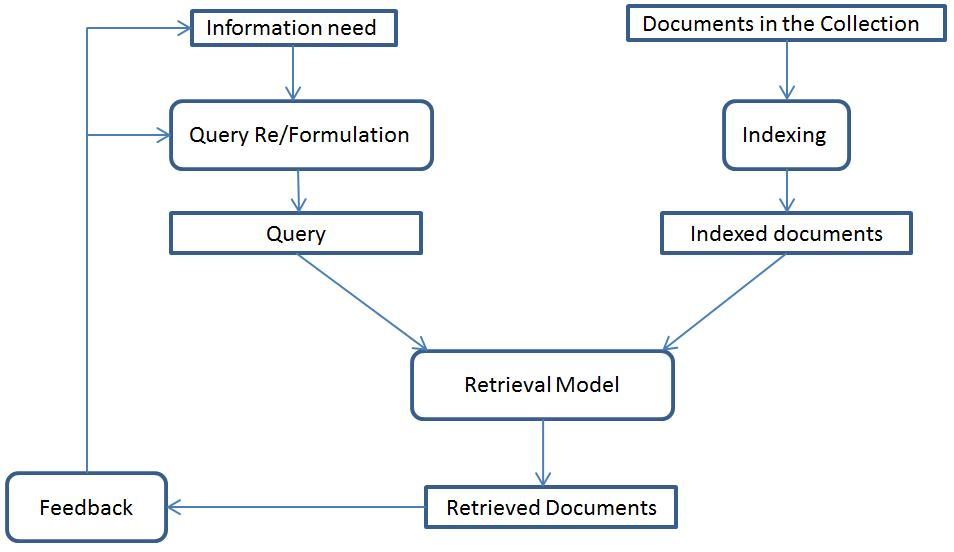
\includegraphics[width=.60\textwidth,height=50mm]{figs/generalIR.jpg}
   \caption{Simple illustration of the process in a general IR system.}  
   \label{fig:generalir} 
\end{figure}
\FloatBarrier 

\subsection{Retrieval Models}
\label{subsub:retmodels}
%Having constructed an index on a document collection, queries need to 
be matched to documents and a list of answers returned. We need a ranking algorithm based on good mathematical retrieval models to 
return relevant documents at top of the ordered list, leading to high effectiveness. 
Three well-known retrieval models are~\citep[p. 233]{croft2010search}: (1) vector space models (e.g., term frequency and inverse document frequency (TF-IDF)), (2) probabilistic models (e.g., BM25\footnote{BM stands for Best Match, and 25 is just a numbering scheme used by~\cite{robertson1994some} to keep track of weighting variants.}), and (3) Language Models~(LM). 

\paragraph{The Vector Space Model}
\ \\
In a vector space model, documents and queries are represented by vectors of term weights, and the collection is represented by a matrix of term weights as follows: 
\begin{displaymath} 
D_{i}=[d_{i1}, d_{i2}, d_{i3}, \ldots , d_{im}],
\end{displaymath}
\begin{displaymath} 
Q=[q_{1}, q_{2}, q_{3}, \ldots , q_{m}],
\end{displaymath}
\begin{displaymath} 
C=
%\begin{matrix} D_{1} \\ D_{2} \\ D_{3} \\ \vdots\\ D_{N} \\\end{matrix}
\begin{bmatrix}
        d_{11} & d_{12} & d_{13} & \cdots & d_{1m}\\
        d_{21} & d_{22} & d_{23} & \cdots & d_{2m}\\
        d_{31} & d_{32} & d_{33} & \cdots & d_{3m}\\
        \vdots\\
        d_{N1} & d_{N2} & d_{N3} & \cdots & d_{Nm}
     \end{bmatrix},
\end{displaymath}
%\capstartfalse
%\begin{figure}[htpb]
%   \centering
%   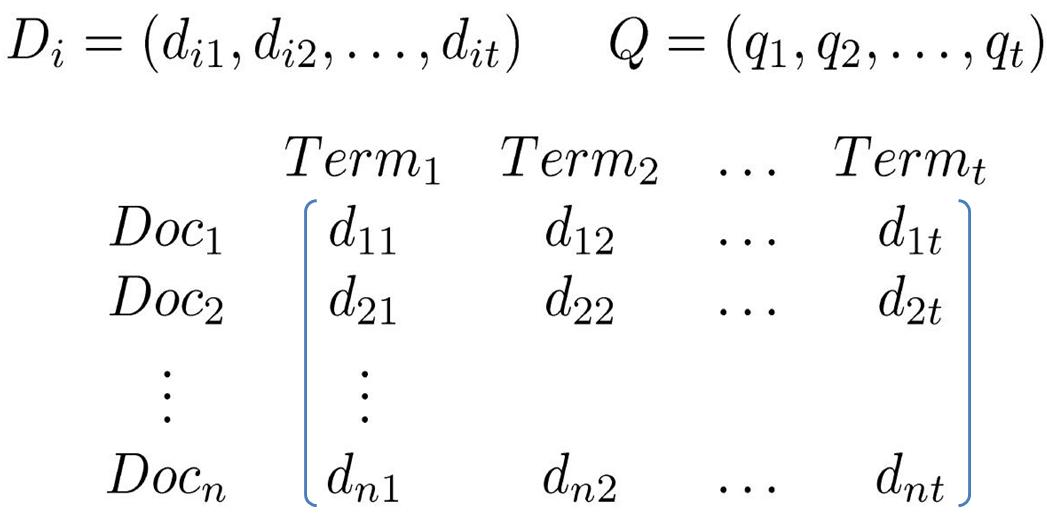
\includegraphics[width=.45\textwidth,height=35mm]{figs/vsm-matrix.jpg}
%\end{figure}
%\capstarttrue
%\FloatBarrier 
\noindent
where $ D_{i} $ is a document in the collection $ C $, $ d_{ik} $ is a weight for each term $ t_{k} $ in the document $ D_{i} $, and $ q_{k} $\footnote{We ignore indices to simplify the further equations in this thesis.} represents a term in the query $ Q $. The collection is represented by the matrix $C_{Nm}$, where $N$ is the number of documents in the collection and $m$ is the number of all vocabularies. If a term does not appear in a document or a query, the weight for that particular term will be zero. 

The TF-IDF weighting function multiplies the occurrence of each term in the document ($ c(t_{k},Di)$)
by the inverse document frequency ($ idf $) measure. $ idf $ measures the importance of a term in the collection: 
\begin{equation}
idf(t_{k})=\log\frac{N+1}{df(t_{k})},
\label{eq:idf}
\end{equation}
where $ df(t_{k}) $ is the number of documents in the collection, which contain at least one occurrence of the term $ t_{k} $, and $ N $ is the number of documents in the collection. 

Given a query $Q$, documents are ranked based on the overlap score measure. The TF-IDF score of a document $D$ is the sum, over all query terms, of the TF-IDF weight of each query term $q$ in $D$. After pivoted normalisation, the TF-IDF score for each document is calculated as follows~\citep{bache2010improving}:
\begin{equation}
TFIDF(Q,D)=\sum\limits_{q \in Q\cap D}\frac{c(q,D)\times idf(q)}{(1-b)+b.\frac{|D|}{avdl}},
\label{eq:tfidf}
\end{equation}
where $ |D| $ is the size of the document (i.e, the number of words) and $ avdl $ is the average document length, $ c(q,D)$ is the number of occurrence of each query term in the document $D$, and $idf(q)$ is the importance of each query term in the collection. TF-IDF model scores a document higher if more query terms are present or these terms are rarer in the collection. The parameter $ b $ is set to 0.75 to be the same as the BM25 model as will be described below.
\paragraph{Probabilistic Models}
\ \\
BM25 is a popular and effective ranking algorithm, which extends the scoring function for the binary independence model~\citep[p. 232]{manning2008introduction} to include document and query term weights. Each document is scored based on the BM25 weighting scheme --- often called the Okapi weighting --- as follows:
\begin{equation}
BM25(Q,D)=\sum\limits_{q \in Q\cap D}\Bigg(\log\frac{N+1}{df(q)}\Bigg)\Bigg(\frac{(k_{1}+1)c(q,D)}{k_{1}((1-b)+b.\frac{|D|}{avdl})+c(q,D)}\Bigg).
\label{eq:idfbm25}
\end{equation}
The variable $ k_{1} $ is a positive tuning parameter that calibrates the document term frequency scaling. The setting of $ k_{1}=0 $ corresponds to a binary model (i.e., no term frequency), and setting a large value for $ k_{1} $ corresponds to using raw term
frequency. The parameter $ b $ is also used for tuning ($ 0 \leq b \leq 1 $) which determines the scaling by document length: $ b = 1 $ corresponds to fully scaling the term weight by the document length, while $ b = 0 $ corresponds to no length normalisation. 

If the query is long, then we might also use similar weighting for query terms. This is appropriate if the queries are paragraph long information needs, but unnecessary for short queries. 
In this case, BM25 weighting function is calculated as follows:
\begin{equation}
BM25(Q,D)=\sum\limits_{q \in Q\cap D}\log\Bigg(\frac{N+1}{df(q)}\Bigg)\Bigg(\frac{(k_{1}+1)c(q,D)}{k_{1}((1-b)+b\frac{|D|}{avdl})+c(q,D)}\Bigg)\Bigg(\frac{(k_{3}+1)c(q,Q)}{k_{3}+c(q,Q)}\Bigg),
\label{eq:idfbm25}
\end{equation}
where $ c(q,Q) $ is the frequency of term $ q $ in the query $ Q $, and $ k_{3} $ being another positive tuning parameter that this time calibrates term frequency scaling of the query. In the equation presented, there is no length normalisation of
queries because retrieval is being done with respect to a single fixed query. The tuning parameters of these equations should ideally be set to optimise performance on a development test collection. That is, we can search for values of these parameters that maximise performance on a separate development test collection (either manually or with optimisation methods such as grid search or something more advanced), and then use these parameters on the actual test collection. In the absence of such optimisation, experiments have shown reasonable values are to set $ k_{1} $ and $ k_{2} $ to a value between 1.2 and 2, and b = 0.75~\citep{manning2008introduction}.
\paragraph{Language Models with Terms Smoothing}
\ \\
The basic idea behind the \textit{Language Modelling} approach is to estimate a language model for each document, and rank documents by the likelihood of the query according to the estimated language model. Here terms are assumed to occur independently, and the probability is the product of the individual query terms given the document model $ M_{D} $ of document $ D $:
\begin{equation}
\label{eq:multinomial}
 P(Q|M_{D}) = \prod\limits_{q\in Q} P(q|M_{D}) 
\end{equation}

\begin{equation}
\label{eq:multinomial}
 P(q|M_{D}) = \frac{c(q,D)}{|D|}
\end{equation}

The overall similarity score for the query and the document could be zero if some of query terms do not occur in the document. However, it is not sensible to rule out a document just because a single query term is missing. For dealing with this, language models make use of smoothing to balance the probability mass between occurrences of terms in documents, and terms not found in the documents.
\\\\
\textit{Jelinek-Mercer smoothing.} Jelinek-Mercer smoothing language model~\citep{zhai2004study} combines the relative frequency of a query term $ q\in Q $ in the document $ D $ with the relative frequency of the term in the collection (\textit{C}) as a whole. With this approach, the maximum likelihood estimate is moved uniformly toward the collection model probability $ P(q|C) $:
\begin{equation}
P(q|M_{D}) = (1-\lambda)\frac{c(q,D)}{|D|}+\lambda P(q|C) 
\label{eq:jmsmoothing}
\end{equation} 
$ c(q,D) $ represents the frequency of term $ q $ in document $ D $. The optimal value of $ \lambda $ depends on both the collection and the query. It is normally suggested as ($ \lambda = 0.1$) for title queries and ($ \lambda = 0.7$) for long queries.
\\\\
\textit{Dirichlet (Bayesian) smoothing (DirS).} As long documents allow us to estimate the language model more accurately, Dirichlet smoothing ~\citep{zhai2004study} smooths them less. If we use the multinomial distribution to represent a language model, the conjugate prior of this distribution is the Dirichlet distribution. This gives:
\begin{equation}
\label{eq:bayessmoothing}
 P(q|M_{D}) = \frac{c(q,D) + \mu P(q|C)}{|D| + \mu}
\end{equation} 

The formula assign negative score to documents that contain the term, but with fewer occurrence than predicted by the collection language model. As $ \mu $ gets smaller, the contribution from the collection model also becomes smaller, and more emphasis is given to the relative term weighting. Precision is more sensitive to $ \mu $ for long queries, especially when $ \mu $ is small. When $ \mu $ is sufficiently large, long queries perform better than short queries. The optimal value of $ \mu $ varies from collection to collection, though in most cases, it is around 2000. The performance is more sensitive to smoothing for verbose queries. Long queries also require more aggressive smoothing to achieve optimal performance. 


\subsection{The Study of Retrievablity}
%Retrievability measures indicate how easily a document could be retrieved using a given IR system, while findability measures indicate how easily a document can be found by a user with the IR system~\citep{azzopardi2008retrievability}. Some documents are retrieved by many queries while others may never show up within the top-n ranked results via any query terms that they are relevant for~\citep{lupu2013patent}. When a document is difficult or impossible to retrieve in a particular retrieval model, it is difficult or impossible to retrieve when relevant and this leads to a low recall. 

Essentially, it is desirable that the retrieval system consider all documents with similar retrievability (Gini-Coefficient is used to measure the retrievability) because documents become less retrievable when others become more retrievable. However, two aspects can affect findability: the inherent bias favouring some types of documents over others introduced by the retrieval model, and the failure to correctly capture and interpret the context~\citep{bashir2009improving, bashir2011relationship}. There are certain features that increase access to the corpus by making the retrievability of documents more equal~\citep{bache2010improving}:
\begin{enumerate}
\item Sensitivity to term frequency: A higher frequency of a given query term makes the document more relevant.
\item Length normalization: Incorporation term frequency into a model make it biased to score longer documents higher than shorter documents, so there is a tendency to over-score longer documents. Shorter documents are not penalised when length normalisation is used.
\item Convexity: An IR model will have convexity if it ranks document $ d_{3} $, which has both query words $ w_{1} $ and $ w_{2} $, higher than documents $ d_{1} $ and $ d_{2} $, which just have one of the query words twice. 
\end{enumerate}
Bias of retrieval systems is the characteristic of a system to give preference to certain features of documents, when it ranks results of any given query. For example, \textit{PageRank} favours popular documents by evaluating the number of in-links of web pages in addition to pure content features while \textit{TFIDF} and \textit{OKAPI-BM25} favour large terms frequencies~\citep{bashir2011relationship}.
\paragraph{Retrievablity Measurement}
\ \\
\textit{Retrievability} measures how likely each document $ d $ inside a collection $ D $ can be retrieved within the top c ranked results for all queries in $ Q $. $ r(d) $ defines as follows:
\[
r(d)=\sum_{q \in Q}f(k_{dq},c)
\]
where $ k_{dq} $ is the rank of $ d $ in the result set of query $ q \in Q $, $ c $ denotes the maximum rank that a user is willing to proceed down the ranked list. The function $ f(k_{dq},c) $ returns a value of 1 if $ k_{dq} \leq c $, and 0 otherwise. \textit{Retrievability} inequality can be analysed using the \textit{Lorenz} Curve. Documents are sorted according to their retrievability score in ascending order, plotting a cumulative score distribution. If the retrievability of documents is distributed equally, then the Lorenz Curve will be linear. The more skewed the curve, the greater the amount of inequality or bias within the retrieval system. The Gini coefficient $ G $ is used to summarize the amount of bias in the Lorenz Curve, and is computed as follows:
\begin{equation}
G=\frac{\sum_{i=1}^n(2.i-n-1).r(d_{i})}{(n-1)\sum_{j=1}^nr(d_{j})}
\end{equation}
\noindent
where $ n=|D| $ is the number of documents in the collection sorted by $ r(d) $. If $ G=0 $, then no bias is present because all documents are equally retrievable. If $ G=1 $, then only one document is retrievable and all other documents have $ r(d)=0 $. By comparing the Gini-Coefficients, we can analyse the retrieval bias imposed by the underlying retrieval functions on a given document collection.

\label{subsub:retrievability}

\subsection{Query Expansion (QE)}
%One solution to the significant term mismatch between the query and the relevant documents is query expansion (QE)~\citep{Efthimiadis1996}, which has been effective in many retrieval tasks. The idea of QE is to add more terms to the original user's query to increase the probability of matching of the query terms with relevant documents, with the objective of improving retrieval effectiveness. The expansion terms can be selected from a feedback process or from external sources such as Wikipedia, or dictionaries~\citep{cao2008selecting}. Original queries should be expanded by good terms, unless it can lead to retrieval of irrelevant documents.
\paragraph{Feedback-based Query Expansion}
\ \\
An initial query can be expanded using a feedback from users --- relevance feedback --- or automatically from top $ k $ ranked retrieved documents, assuming they are relevant to the query --- pseudo relevance feedback (PRF)~\citep{manning2008introduction}. Getting feedback from  users needs user studies and interaction while pseudo relevance feedback is an automated process without user interaction.
\begin{figure}[t!]
%[htpb]
   \centering
   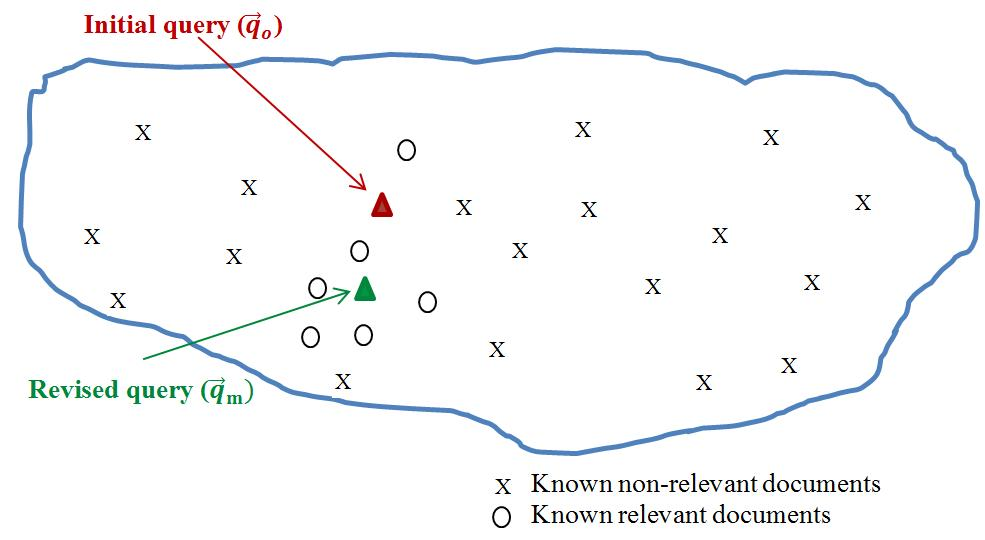
\includegraphics[width=0.65\textwidth,height=50mm]{figs/rocchio.jpg}
   \caption{Rocchio algorithm for relevance feedback. Some documents have been labelled as relevant and irrelevant and the initial query vector is moved in response to this feedback~\citep{manning2008introduction}.}  
   \label{fig:rocchio} 
\end{figure}
\FloatBarrier 
%\noindent
\textit{The Rocchio Algorithm for Relevance Feedback}: The Rocchio
algorithm \citep{Salton1971} is a classic algorithm of relevance feedback
used mainly for query expansion. In brief, it provides a method of
incorporating relevance feedback information into the vector space
model representing a query~\citep{manning2008introduction}. 
The Rocchio algorithm is used to modify the query by the partial knowledge of known relevant and irrelevant~\footnote{In this thesis, we use irrelevant and non-relevant interchangeably for documents that are not relevant to the query.} documents; the goal is to move the query closer to the centroid of the relevant documents but further from irrelevant documents (Figure \ref{fig:rocchio}). The modified query $ \vec{q}_m $ is:
%\[ 
\begin{equation}
\label{eq:rocchio}
 \vec{q}_{m} = \alpha  \vec{q}_{0} + \beta\frac{1}{|D_{r}|}\sum\limits_{\vec{d_{j}}\in D_{r}} \vec{d_{j}} - \gamma\frac{1}{|D_{irr}|}\sum\limits_{\vec{d_{j}}\in D_{irr}} \vec{d_{j}},
  \end{equation}
 %\tag{2.1}\label{eq:rocchio}
 %\]  
where $ q_{0} $ is the original query vector; $ D_{r} $ and $ D_{irr} $ are the set of known relevant and irrelevant documents, respectively; and $ \alpha $, $ \beta $, and $ \gamma $ are weights attached to each term. These control the balance between trusting the judged document set versus the query: if we have a lot of judged documents, we
would like higher $ \beta $ and $ \gamma $~\citep{manning2008introduction}. 

PRF is typically used in Rocchio algorithm. However, it is important to distinguish between good expansion terms and bad ones. Distinguishing between expansion terms only based on their distribution in the feedback documents (i.e., extracting the most frequent terms) and in the whole collection (i.e., extracting the most specific terms) is not sufficient. It can be considered as a term classification problem to separate good expansion terms from others directly according to their potential impact on the retrieval effectiveness; hence, we can apply supervised learning methods for term selection. Classifiers like support vector machines (SVM)~\citep{cao2008selecting}, Na\"ive Bayes and Logistic Regression~\citep{he2009finding} can be used to classify terms and feedback documents.  
\paragraph{Query Expansion by External Resources}
\ \\
The most common form of query expansion is a global analysis, using dictionaries, WordNet, Wikipedia, or other thesaurus. For each term $ t $ in a query, the query can be automatically expanded with synonyms and related words of $ t $ from the thesaurus. Use of a thesaurus can be combined with ideas of term weighting; for instance, one might weight added terms less than original query terms~\citep{manning2008introduction}.

\subsection{Query Reduction (QR)}
%In general, retrieval effectiveness for long queries is often lower than retrieval effectiveness for shorter keyword queries because the additional information provided in verbose queries is more likely to confuse current search engines rather than help them. Query reduction (QR), a technique for dropping unnecessary query terms from long queries, improves the performance. 

A common approach to reduce verbose queries is selecting a subset of a long query (or sub-query). A search engine performs more precisely when just the key concepts are used as a query rather than a long query. Hence, the identification of the key query concepts has a positive impact on the retrieval performance for verbose queries. Extracting the key query concepts can be done by learning to identify key concepts in long queries using a variety of features~\citep{bendersky2008discovering}. We can choose effective subsets in a query by analysing all the subsets of terms from the original query (sub-queries), and identifying the most promising sub-query to replace the original long query. For ranking sub-queries, an algorithm based on the SVM classification is used~\citep{kumaran2009reducing}. In this approach, the quality of query reduction depends on the performance of the predictor and ranking algorithm~\citep{balasubramanian2010exploring}. 

As the other approach, we can use query term ranking techniques to select effective terms from a verbose query by ranking them. A vast number of rankings are possible given different settings of individual term weights; for example, we can train a regression model to weight all query words of a verbose query~\citep{lease2009regression}. We can also assign weights to concepts by learning the importance of concepts underlying
the verbose query~\citep{bendersky2010learning}.

%\subsubsection{Query Reformulation}
%\input{query_reform}

\subsection{IR Evaluation Metrics}
%A retrieval system is evaluated considering a set of relevance judgements, a binary assessment of either \textit{relevant} or \textit{irrelevant} for each query-document pair. An ideal retrieval system can retrieve all relevant documents. Table \ref{tab:contengency} is the contingency table, where:\\\\
\textit{True Positive (tp)}: documents which are relevant and the system retrieves them.\\
\textit{False Negative (fn)}: documents which are relevant but the system does not retrieve them. \\
\textit{False Positive (fp)}: documents which are non-relevant but the system retrieves them.\\
\textit{True Negative (tn)}: documents which are non-relevant and the system does not retrieve them. 
\begin{table*}[htpb]
  \centering
  \input table/contingency.tex
  \caption{Contingency table.}
  \label{tab:contengency}
\end{table*}
\FloatBarrier 
\paragraph{Precision and Recall}
\ \\
Precision and recall are the most frequent and basic measures for information retrieval effectiveness. They are calculated with respect to what IR system returns as a set of documents for a query.\\
\textit{Precision (P)} is the fraction of retrieved documents that are relevant:
\[
Precision (P)=\frac{\sharp(relevant \: items \: retrieved)}{\sharp(retrieved \: items)}=\frac{tp}{tp+fp}=P(relevant|retrieved)
\]
\textit{Recall (R)} is the fraction of relevant documents that are retrieved:
\[
Recall (R)=\frac{\sharp(relevant \: items \: retrieved)}{\sharp(relevant \: items)}=\frac{tp}{tp+fn}=P(retrieved|relevant)
\]
For many prominent applications, particularly web search, good results on the first page or the first three pages are important than all relevant documents. So, they wish to look at precisions and recalls over a series of different rank cut-offs rather than to look at the entire retrieved set. This is referred to as ``Precision/Recall at k'', for example ``Precision/Recall at 10''. 
\begin{equation}
precision@k=\frac{\sharp(documents \: retrieved \: and \: relevant \: up \: to \: rank \: k)}{k}
\end{equation}
\begin{equation}
recall@k=\frac{\sharp(documents \: retrieved \: and \: relevant \: up \: to \: rank \: k)}{\sharp(documents \: relevant)}
\end{equation}
\paragraph{Average Precision and Mean Average Precision (MAP) }
\ \\
We can measure MAP by calculating Average Precision on retrieval results. Average Precision is the average of precision at each point where a relevant document is found is computed as:
\begin{equation}
Avg. \: precision=\frac{\sum_{r=1}^{N}(P(r)\times rel(r))}{n}
\end{equation}
\noindent
where $ r $ is the rank, $ N $ the number of documents retrieved, $ rel(r) $ a binary function of the document relevance at a given rank, $ P(r) $ is precision at a given cut-off rank $ r $, and $ n $ is the total number of relevant documents.

Then, for a given set of queries, $ Q $, $ MAP $ can be calculated by:
\begin{equation}
MAP(Q)=\frac{\sum_{q\in Q}Avg. \: precision(q)}{|Q|}
\end{equation}
\noindent
where $ q $ is a query in a set of queries $ Q $.

%------------------- Patent-specific IR ---------------------

\section{Patent-specific IR}
\label{subsec:patentir}

\subsection{The Study of Retrievablity for patents}
%Rerievability is specifically critical in recall oriented applications like patent retrieval or legal settings. In these cases, the focus of a system is to retrieve all documents that are relevant rather than to retrieve a subset of documents that the best satisfy the query intent.
Hence, all documents should at least potentially be retrievable via correct query terms. Designing retrieval systems for recall oriented tasks has been emphasised in recent years~\citep{fujii2007introduction, kontostathis2008effect}. Before designing a new or using an existing retrieval system for recall oriented applications, one needs to analyse the effects of the retrieval system bias as well as the overall retrievability of all documents in the collection using the retrieval function at hand.

In retrievability, we analyse documents specifically with respect to relevant and irrelevant queries to identify whether highly retrievable documents are really highly retrievable, or whether they are simply more accessible from many irrelevant queries rather than from relevant queries. Experiments show that about 90\% of patent documents which are highly retrievable across all types of queries, are not highly retrievable on their relevant query sets~\citep{bashir2009analyzing}.

Experiments with different collections of patent documents suggest that query expansion with pseudo relevance feedback can be used as an effective approach for increasing the findability of individual documents and decreasing the retrieval bias. Pseudo relevance feedback documents are identified using cluster-based~\citep{bashir2009improving} or terms-proximity-based methods~\citep{bashir2010improving}.

Another study~\citep{bache2010improving} analyses the relationship between retrievability and effectiveness-based measures (Precision, MAP). Results show that the two goals of maximising access and maximising performance are quite compatible. They further conclude that a reasonably good retrieval performance can be obtained by selecting parameters that maximise retrievability (i.e., when there is the least inequality between documents according to Gini coefficient given the retrievability values). Their results support the hypothesis that retrieval functions can be effectively tuned using a retrievability-based measure without recourse to relevance judgments, making it an attractive alternative for automatic evaluation.


\subsection{Query Formulation}
%%Query or topic is the the request for information in any retrieval system. An effective query can lead in retrieving the required information. Queries formulated by users are not usually optimal for retrieval process, therefore, they need to be transformed by techniques such as query expansion or query reduction. 
The patent prior art search begins with a full patent application as a query. A full text as a query is a challenge compared to a classical IR, since it is not focused on the information that the user needs. In order to achieve good retrieval results, it is important to extract the best representative text with the proper weights. Therefore, query generation based on query document is essential to reduce the difficulty of formulating effective queries by users. 
%The query created before the retrieval can be modified or enhanced after retrieval. In this section, the initial query formulation will be discussed and in the next section, post-retrieval query reformulation will be covered. 
\\\\
\textbf{Which fields in patent application are more effective to extract query terms}
\ \\
A special characteristic of patent documents is their structural information. They mainly have different fields such as title, abstract, description, and claims. Different fields use different type of language for describing the invention. Abstract and description use more technical terminology while claim field usually uses a legal jargon. Structured indexing keeps the field structure in the index, which allows searching specific fields instead of searching in full document. Separate fields for meta-data (Section \ref{sec:metadata} ) like IPC code and author can help to retrieval effectiveness~\citep{magdy2010exploring}. 

Early patent search tasks mainly considered claims to build the query, the same as what examiners start the novelty process~\citep{konishi2005query, takaki2004associative, mase2005proposal, fujii2007enhancing}, whereas recent works have showed that building queries from description field is more useful in patent retrieval (considering background summary in US patents equivalent to description field in European patents.)~\citep{xue2009transforming, xue2009automatic, mahdabi2011building}. Another research showed that extracting terms according to $ log(tf)idf $ scores from every field of the query patent, and giving higher importance to terms extracted from the abstract, claims, and description fields than to terms extracted from the title field, is an effective way of constructing a search query~\citep{cetintas2012effective}. The other experiment showed that discarding description from query improves MAP up to 30\% because the description contains more noise than information~\citep{gobeill2010simple}. They also showed that claims are more informative and title is poorly informative in retrieval.   


\paragraph{Using Phrases instead of Terms}
\ \\
Most of query formulation techniques rely on terms, but encouraging results have been obtained using phrases recently~\citep{becks2010phrases}. Early results demonstrated that an NLP-based grouping of terms can increase the performance compared to the bag-of-words approach, though the increase is smaller than in a non-patent collection~\citep{osborn1997evaluating}. Another task could improve retrieval effectiveness by adding syntactic phrases in the form of dependency triples, to a bag-of-words representation~\citep{d2011combining}. Key Phrase Extraction (KPE) algorithms is another way to form a query based on phrases. A list of phrases, generated by a KPE algorithm, can succinctly represent a complex and lengthy patent. ~\citep{verma2011applying}.

\paragraph{Diverse Query Generation}
\ \\
In this approach, the focus is on generating diverse queries that can improve overall retrieval effectiveness in sessions rather than generating a single best query that can retrieve more relevant documents from a single retrieval result (i.e., more relevant documents in aggregated retrieval results obtained by multiple queries in a session). Diverse query generation is important because query documents typically contain several different aspects (or topics) and different types of relevant documents may be related to these aspects. To identify aspects, 500 top terms based on their tf-idf rank, are clustered into $ n $ sets with respect to their similarity. Each distinct sets of terms represents one query aspect, then top $ k $ retrieved documents for each sub-query consider as pseudo-relevant documents (PRD) and those ranked below the top $ k $ are non-relevant documents (NRD). Then the query is generated by decision tree. ~\citep{kim2014searching, kim2014diversifying}.

\subsection{Query Expansion for Patents}
%Although a query is very long in patent prior art search, a significant term mismatch between queries and relevant documents has reported in~\citep{roda2010clef, magdy2010exploring}. The QE is a suggested solution to cope with the term mismatch problem; however, most of the QE techniques were ineffective to improve the performance in patent domain~\citep{kishida2003experiment, konishi2005query}. We review previous works on the QE techniques for the patent search here.
\paragraph{Query Expansion by Pseudo Relevance Feedback}
\ \\
Previous studies~\citep{magdy2011study} have discussed that PRF is ineffective for patent prior art search. Since the retrieval effectiveness is low at initial retrieval, the assumption that top $ k $ documents are relevant is invalid and leads in adding noise to the query; hence, the improvement using PRF is insignificant. The solutions proposed to cope with this problem are as follows:
\begin{list}{-}{}
\item \textbf{Selecting documents for PRF based on cluster analysis:} In this approach, a document that can cluster lots of high similar documents is considered relevant and a document that has no nearest neighbour or some neighbours with low similarity is considered irrelevant~\citep{lee2008cluster}. In patent domain, where there is a large vocabulary diversity for expressing an invention, the idea can be improved by intra-cluster similarity rather than only on the basis of their size~\citep{bashir2009improving}. 
\item \textbf{Selecting patents for PRF based on their similarity with query patent via specific terms:} In this approach, patents for PRF are identified based on their similarity with query patents over a subset of terms, rather than the overall document similarity. The success of this approach highly depends on selecting appropriate terms from patent query, which produce the best PRF candidates that can help in improving retrievability during QE~\citep{bashir2010improving}. Experiments show a significant improvement for Gini coefficient, which is used to measure retrievability, but there is no report on other main measures (e.g., MAP and recall).
\item \textbf{Identyfying expansion terms: } 
\ \\
Term proximity information can be used to identify expansion terms. Given a patent query, first, an initial query is generated by taking, for example, claim terms; then a query-specific lexicon based on definitions of the IPC is created.
Among many terms in the lexicon, only expansion terms identified by two adjacency operators used in patent examination\footnote{Patent examiners use term proximity heuristics in their
searches in Boolean retrieval model in order to reward a
document where the matched query terms occur close to
each other. Two forms of adjacency operators are used in
Boolean retrieval model to address proximity. `ADJn' operator which searches for terms within \textit{n} words proximity in
the order specified, and `NEARn' operator, which searches
for the terms within \textit{n} words, in either order.} (i.e., `ADJn' and `NEARn') are used for query expansion~\citep{mahdabi2013leveraging}.
\item \textbf{Predicting the effectiveness of feedback documents: } 
\ \\
In patent retrieval, the MAP is very low at initial retrieval; hence the top retrieved documents are not essentially relevant. 
As a result, there is a high
chance that we use irrelevant documents for expansion in PRF. Recently,
machine learning methods like regression are used to improve the PRF by predicting the effectiveness of a feedback document~\citep{mahdabi2012learning}.
\end{list}
Random indexing to identify terms to use for query expansion~\citep{sahlgren2002english} and expansion using noun phrases~\citep{mahdabi2012automatic} are the other techniques to improve the effectiveness of standard query expansion for prior art search. 
\paragraph{Query Expansion by External Resources}
\ \\
Some external resources like WordNet~\citep{miller1990introduction}, which were reported to improve retrieval effectiveness in several IR research investigations, show insignificant change to overall retrieval effectiveness, but a degree of improvement for some topics in patent domain. \cite{magdy2011study} applied the idea of automatically generating the synonyms set (SynSet) using parallel manual translations to create possible synonyms sets (in CLEF-IP collection, some sections in some patents are translated into three languages: English, French, and German). Although this idea presents better results compared to WordNet, there is still a little improvement in retrieval effectiveness. The only QE task, which achieves the best results, uses a combination of PRF and QE with translation of terms and phrases from German and French~\citep{jochim2011expanding}.


\subsection{Query Reduction for Patents}
%Query reduction is a solution for problems with using a full verbose patent as a query: it is not focused on information needed by the user, and a verbose query may cover more than one topic.

\begin{list}{-}{}

\item \textbf{Query Segmentation :} Decomposing each patent query into coherent sub-topics segments-using TextTiling~\citep{hearst1997texttiling}-is a solution to make long ambiguous queries focused on the information need. Sub-topic segments can be used as separate queries (query stream) for initial retrieval, then the retrieval results from each of the individual streams are merged to construct the final ranked list for the whole original query. Using each sub-topic as a query stream enables a retrieval model to retrieve related documents from the collection in a more precise way and also allow the PRF algorithm to work on a more focused set of pseudo-relevant documents~\citep{takaki2004associative, ganguly2011united}. Another work adapted pseudo relevance feedback for query reduction by decomposing a patent application into constituent text segments and computing the Language Modelling (LM) similarities by calculating the probability of generating each segment from the top ranked documents. The least similar segments from the query removed from the query, hypothesizing that removal of segments most dissimilar to the pseudo-relevant documents can increase the precision of retrieval by removing non-useful context, while still retaining the useful context to achieve high recall as well~\citep{ganguly2011patent}.

\item \textbf{Patent Summarization :} This approach assumes that the patent summary (using TextTiling) reflects the main topic as well as the subtopics of a patent document in a concise manner. Then, language model for the query, collection, and each summary are generated~\citep{mahdabi2011report}. 

\end{list}



%\subsubsection{Query Reformulation for Patents}
%\input{query-reform-p}

\subsection{The Use of Metadata}
%The main textual content of patent documents is known to be difficult to process with traditional text processing and text retrieval techniques, but patents contain additional material, such as: tables, mathematical and chemical formulas, citations, technical drawing, meta-data, e.g., applicant, inventor, Intentional Patent Classification (IPC) codes, and publication date, that can be used to improve the retrieval. In this section, the use of patent meta-data to improve the retrieval has been explained.
\paragraph{The Use of Citation}
\ \\
The most successful use of metadata to date is the citation lists in order to learn patterns of relevance ~\citep{lupu2013patent}. The patent collection is a very dense network of citations creating a set of interrelations particularly interesting to exploit during a prior art search. The large majority of patents are continuations of previous works and patents. The citation relations make this development process
visible. Similarly, fundamental patents which open new technologies sub-fields are exceptional but tends to be cited very frequently in the whole sub-field during years. Citation graph of a patent collection is used for identifying patent thickets, i.e. the patent portfolios of several companies overlapping on a similar technical aspect. Related patents can be inferred from the overall citation network of a patent collection. If a new patent applicant belonging to this patent ticket appears, it is very likely that the most relevant prior art documents are already
present in this patent thicket~\citep{lopez2009multiple}.

The patents cited in the description of the topic patent are used as relevant documents, because citations are usually prior arts for a citing patent. Only citations which are in the collection can be helpful in the retrieval process. The idea of \textit{PageRank}-identifying authoritative pages by analysing hyperlink structure on World Wide Web\_ can be used for citations. A patent, which is cited by a large number of other patents, is more important. Text-based and citation-based scores combined to compute the ranking score for documents~\citep{fujii2007enhancing, fujii2007integrating}.

Citation texts for patents are a whole paragraph. Therefore, for each patent document presented and cited in the collection, the entire paragraph of citation can be appended to the textual material of the cited patent. A boolean feature uses to indicate weather a cited patent in query patent has retrieved, then this document can get a higher weight at any future post-ranking process. Due to the limited number of citation texts, this approach showed just a trivial improvement~\citep{lopez2009multiple}. However, citation information does not always presented in the patent application and this method can not be used in real life patent search and initial citations by the applicants may not consider relevant by patent examiners~\citep{magdy2010applying, magdy2011simple}. 

Similar tasks also indicated improvement in 'MAP' and 'Recal' using citations in patent retrieval~\citep{gobeill2010simple, gurulingappa2010prior}. 
\paragraph{The Use of IPC Codes}
\ \\
Patents are classified by the patent offices into large hierarchical classification schemes based on their area of technology. The use of patent
classification has two major benefits. The first is that the classifications provide access to concepts rather than words, such that even
if the same word or phrase is commonly used in two technology areas, patent classifications will provide the context of its use. In effect, they
allow the search space of patents to be reduced, by allowing the user to exclude from the search process patents in classes not related to
the search topic at hand~\citep{lopez2010patatras}. The second major benefit is the language independence provided by classifications, as classification symbols can be mapped to multiple languages~\citep{DBLP:conf/clef/DhondtV10}. This allows patent searchers to conduct reasonably effective retrieval even in languages that they do not understand. All previous works, considered IPC code in their search, reported improvement in retrieval effectiveness~\citep{harris2010comparison, harris2011using, harris2009role, fujita2005revisiting, graf2010knowledge, herbert2010prior, kang2007cluster, verma2011applying}. It has also reported that using complete IPC code leads in better results than just 4-digit code~\citep{ gobeill2010simple}.
\paragraph{The Use of Images}
\ \\
For the purposes of the search for innovation, we are interested in all forms of information. Some technology areas rely information present in images (flowcharts and diagrams), so, beyond text data, image processing tasks also can contribute to the search. Graph-based measure has a higher discriminative power, but higher computational costs than the text-based measures~\citep{lupu2013evaluating}.

\label{sec:metadata}

\subsection{Multilinguality}
%The interest in multilingual patent search arises from their international and multilingual nature (the European patent office-EPO-makes patent text available in three languages: English, French, and German). Patents on the same topic may be published in different countries in different languages, and it is important for patent examiners to be able to locate relevant existing patents whatever language they are published in. Therefore an important topic in patent retrieval is Cross-Language Information Retrieval (CLIR), where the topic is a patent application in one language and the objective is to find relevant prior-art patents in another language ~\citep{lupu2013patent,joho2010survey, roda2010clef, DBLP:conf/clef/PiroiLHSMF12}. In recent years machine
translation (MT) has become established as the dominant technique for translation in CLIR, which usually achieve better CLIR effectiveness than dictionary-based translation (DBT) methods. However, translation using MT is time consuming and resource intensive for cross language patent retrieval (CLPR), where the query text can often take the form of a full patent application running to tens of pages. Applying IR text pre-processing like stop word removal and stemming to the MT training corpus prior to the training phase can lead to a significant decrease in the MT computational~\citep{magdy2013studying}.




\subsection{Multi-stage Retrieval}
It is common to use patent meta-data and non-textual features as pre and post processing steps of text-based retrieval techniques~\citep{lopez2009multiple}. Many patent retrieval tasks re-rank the top retrieved documents from initial retrieval stage based on additional patent feature ~\citep{lopez2010experiments}, claim structure ~\citep{mase2005proposal}, and considering IPC information of patent and its neighbours to retrieve similar patents~\citep{verma2011exploring}. 

\subsection{Evaluation Metrics for Patent Retrieval}
%The simplest solution to measure the performance in a recall focused IR task is to evaluate the recall, however, it fails to reflect how early a system retrieves the relevant documents and without precision, returning a perfect recall is invalid~\citep{Suominen08t.:critical}. Although recall is the objective for such applications, the score should be able to distinguish between systems that retrieve relevant documents earlier than those that retrieve them later. For recall-oriented IR applications, the problem is viewed as a ranking problem with a cut-off for a maximum number of documents to be checked $ N_{\max} $.\\\\
\textbf{Patent Retrieval Evaluation Score}
\ \\
\begin{figure}[t!]
   \centering
%   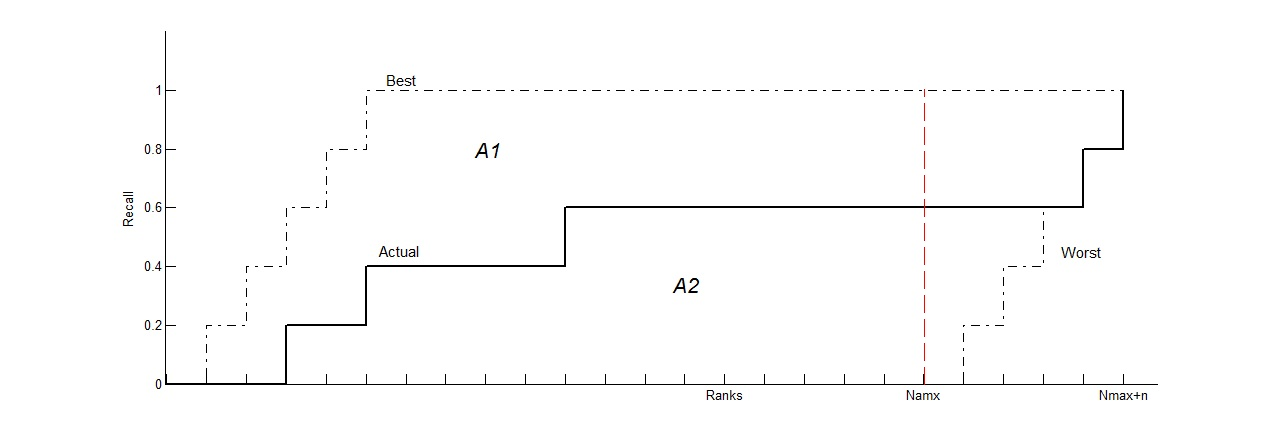
\includegraphics[width=1\textwidth,height=50mm]{figs/pres.jpg}
   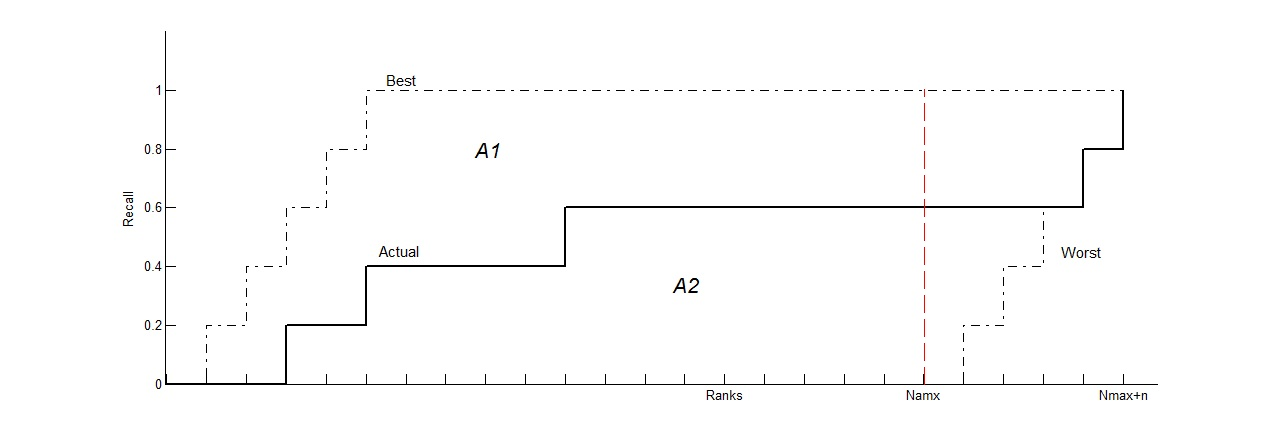
\includegraphics[scale=.37]{figs/pres.jpg}
   \caption{PRES curve is bounded between the best case and the new defined worst case~\citep{magdy2010pres}.}  
   \label{fig:pres} 
\end{figure}
%\FloatBarrier 
Patent retrieval evaluation score (PRES)~\citep{magdy2010pres} is a novel metric for evaluating recall-oriented IR applications, which derived from the normalised recall measure ($ R_{norm} $). It measures the ability of a system to retrieve all known relevant documents earlier in the ranked list. Unlike MAP and recall, PRES is dependent on the relative effort exerted by users to find relevant documents. This is mapped by $ N_{\max} $ (Equation \ref{eq:pres}), which is an adjustable parameter that can be set by users and indicates the maximum number of documents they are willing to check in the ranked list. PRES measures the effectiveness of ranking documents relative to the best and worst ranking cases, where the best ranking case is retrieving all relevant documents at the top of the list, and the worst is to retrieve all the relevant documents just after the maximum number of documents to
be checked by the user ($ N_{\max} $). The idea behind this assumption is that getting any relevant document after $ N_{\max} $ leads to it being missed by the user, and getting all relevant documents after max leads to a zero recall, which is the theoretical worst case scenario. 
%Figure 1 shows an illustrative graph of how to calculate PRES, where 
PRES is the area between the actual and worst cases ($ A_{2} $) divided by the area between the best and worst cases ($ A_{1}+A_{2} $).
$ N_{\max} $ introduces a new definition to the quality of ranking of relevant results, as the ranks of results are relative to the value of $ N_{\max} $. Any relevant document not retrieved in the top N max is assumed to be the worst case (Figure~\ref{fig:pres}).
For example, getting a relevant document at the rank 10 will be very good when $ N_{\max}=1000 $, good when $ N_{\max}=100 $, but bad when $ N_{\max}=15 $, and very bad when $ N_{\max}=10 $. Systems with a higher recall can achieve a lower PRES value when compared to systems with a lower recall but a better average ranking. The PRES value varies from $ R $ to $ \frac{nR^{2}}{N_{\max}} $, where $ R $ is the recall, according to the average quality of ranking of relevant documents.
\begin{equation}
\label{eq:pres}
PRES=\frac{A_{2}}{A_{1}+A_{2}}=1-\frac{\frac{\sum r_{i}}{n}-\frac{n+1}{2}}{N_{\max}},
\end{equation}
where $ r_{i} $ is the rank at which the $ i $th relevant document is retrieved, $ N_{\max} $ is the maximum number of retrieved documents to be checked by the user (i.e. the cut-off number of retrieved documents) and $ n $ is the total number of relevant documents.












































At the begging of each chapter, please introduce the motivation and high-level
picture of the chapter. You also have to introduce sections in the
chapter. \\


Section~\ref{sec:motivation} xxxx.\\


Section~\ref{sec:relatedwork} yyyy.\\


\section{Motivation}
\label{sec:motivation}


\section{Related work}
\label{sec:relatedwork}
You may reference other papers. For example: 
Generational garbage collection~\citep{LH:83,Moon:84,Ungar:84} is perhaps the
single most important advance in garbage collection since the first collectors
were developed in the early 1960s. (doi: "doi" should just be the doi part, not
the full URL, and it will be made to link to dx.doi.org and resolve.
shortname: gives an optional short name for a conference like PLDI '08.)





\section{Summary}
Summary what you discussed in this chapter, and mention the story in next
chapter. Readers should roughly understand what your thesis takes about by only reading
words at the beginning and the end (Summary) of each chapter.





%\chapter{Data Collection and Baseline Framework}
%\input{Data Collection and Baseline Framework}

\chapter{Baseline Framework}
\label{cha:BaselineIRFramework}
In this chapter, we first briefly explain the baseline system and the experimental settings, 
and we describe the data collection we used --- CLEF-IP. Then we cover two main errors caused by the data curation and experimental settings.
%%%%%%%%%%%%%%%%%%%%%%%%%%%%%%%%%%%%%%%%%%%%%%%%%%%%%%%%%%%%%%%%
%%%%%%%%%%%%%%%%%%%%%%%%%% Section 1 %%%%%%%%%%%%%%%%%%%%%%%%%%%
%%%%%%%%%%%%%%%%%%%%%%%%%%%%%%%%%%%%%%%%%%%%%%%%%%%%%%%%%%%%%%%%
\section{Baseline and Experimental Settings}
\label{sec:settings}
We developed a baseline IR system for patent prior art search on the top of
the Lucene search engine\footnote{\texttt{http://lucene.apache.org/}}, which processes queries using both BM25~\citep{Robertson1993} and LM (Dirichlet
smoothing, and Jelinek-Mercer smoothing)~\citep{zhai2004study} scoring functions. %We consider 
%using BM25F~\cite{robertson2004simple} but had no opportunity to learn appropriate field weights.
We used Lucene to index the English subset of CLEF-IP 2010 dataset\footnote{\texttt{http://www.ifs.tuwien.ac.at/\textasciitilde{}clef-ip/}} 
(We will describe CLEF-IP in section~\ref{sec:DataCollection}) that contains 2.6 million patent documents and 1303 topics (queries) for the English test set.
We used the default Lucene settings using the Porter stemming algorithm \cite{Porter1980} and English stop-word removal. 
We also removed patent-specific stop-words as described in \cite{magdy2012toward}.
In
our implementation, each section of a patent (title, abstract, claims,
and description) is indexed in a separate field. However, when a query 
is processed, all indexed fields are targeted with an equal weight, since this generally
offers best retrieval performance. We also used the International
Patent Classification (IPC) codes assigned to the topics to filter
the search results by constraining them to have common IPC codes with
the patent topic as suggested in previous works~\citep{lopez2010patatras}.
Although this IPC code filter may prevent retrieval of relevant patents 
--- as it will be explained in section~\ref{sec:ClassificationCodeMismatch} ---, we
have chosen to keep it for the following reasons: (i) more than 80\%
of the patent queries share an IPC code with their associated relevant
patents, and (ii) it makes the retrieval process much faster. The accuracy of the results is evaluated 
using two popular metrics --- Mean Average Precision (MAP), Average Recall, and Patent Retrieval Evaluation 
Score~\citep{magdy2012toward} (PRES) --- on the top-100 results for each query, assuming that patent examiners 
are willing to assess the top 100 patents \citep{joho2010survey}. 
We achieved the best performance while querying with the Description
section as in previous work \citep{xue2009transforming} and using
either the LM or the BM25 scoring functions. We call this initial
query the \textit{Patent Query} and use it as our main baseline.
\begin{table*}[htpb]
  \begin{center}
  \caption{Comparing performance metrics for different IR models and query formulation.}
  \input table/IRmodels_Sections.tex 
  \label{tab:IRmodels_Sections}
  \end{center}  
\end{table*}
\FloatBarrier 
\noindent

In addition, we compare our results to \textit{PATATRAS}, a highly engineered system developed by Lopez and Romary~\citep{lopez2010experiments}, which achieved the best performance in the CLEF-IP 2010 competition. This system uses multiple retrieval models (especially Kullback-Leibler divergence~\cite{Baeza-Yates2011} and Okapi BM25) and exploits patent metadata and citation structures.  While our evaluation excludes 22 of the 1303 topics for which no relevant English documents were available, the difference in MAP score between our evaluation and the full 1303 topic evaluation of PATATRAS is negligible. We exclude 22 queries because the focus of our research has been on term analysis and errors related to term matching process of ranking functions. So, we eliminated data curation errors and IPC filter errors--- as they will be described in Section~\ref{sec:DataCurationErrors} and Section~\ref{sec:ClassificationCodeMismatch}--- to increase the accuracy of our data analysis results. 
%did not include errors related to non-English patents in our evaluation and we mainly focus on errors related to term matching for English patents.  
%However, the MAP we provide is not directly comparable since we excluded 22 topics from our evaluation because their relevant patents were not in English or had no IPC code matched with the topic. We pruned these topics out because we were only interested in analysing errors related to term matching. Removing 22 topics caused only 0.04 improvement in our baseline system, which is negligible. Hence, we use Top CLEF-IP 2010 results for a rough comprasion."}
% 

% TODO: Don't exclude 22 topics!

%%%%%%%%%%%%%%%%%%%%%%%%%%%%%%%%%%%%%%%%%%%%%%%%%%%%%%%%%%%%%%%%
%%%%%%%%%%%%%%%%%%%%%%%%%% Section 2 %%%%%%%%%%%%%%%%%%%%%%%%%%%
%%%%%%%%%%%%%%%%%%%%%%%%%%%%%%%%%%%%%%%%%%%%%%%%%%%%%%%%%%%%%%%%
\section{Data Collection}
\label{sec:DataCollection}
The prior art candidate search task (PAC) was introduced in three subsequent years: 2009, 2010, and 2011 by CLEF-IP evaluation track\footnote{\url{http://www.ir-facility.org/prior-art-search1}}. We used CLEF-IP 2010 data collection\footnote{\url{http://www.ifs.tuwien.ac.at/~clef-ip/}}
in our experiments. CLEF-IP 2010 is a set of patents from the `European Patent Office' (EPO), and CLEF-IP 2011 includes the same patent data collection from EPO, but with the addition of a new set of patents from `World Intellectual Property Organization' (WIPO). CLEF-IP 2010 contains 2.6 million patent documents and CLEF-IP 2011 consists of 3 million patent documents. The English test sets of CLEF-IP 2010 and CLEF-IP 2011 correspond to $1,303$ and $1,351$ topics respectively.

Each patent in the collection consists of multiple versions of documents in the XML format, labelled as A1, A2, $\ldots$, B1, and B2. The letter 'A' refers to different versions of patent applications. The 'B' versions refer to granted patents. Each of these versions contains some updates to the text, citations, and claims of previous one. As recommended by~\cite{magdy2012toward}, we merge different versions of a single patent into one single document. The content of each section in the merged document is taken from the latest available versions of documents, which leads to presence of some patents in the collection with many missing content fields. The problem of missing data is in some cases so significant that some of these patents consist only of title.

The patent collections contain material in three different languages: English, German, and French. Granted published version of a patent (i.e., the 'B' version) by the EPO should contain the claims section manually translated into all three languages. In addition, all patents have the title in the three languages. The description section of all patents is always provided in the original submission language only.

Test topics provided are English, German, and French patent applications, which are used as a query for the retrieval system. Topics for CLEF-IP 2010 are patent applications rather than granted patents as in 2009. Therefore, non-English patent applications did not contain any English translations in any section except the title and the abstract. However, in CLEF-IP 2010, $1,302$ out of $1,303$ test topics were English and only one was German. 

Figure~\ref{fig:lang-a} shows the percentage of the English, German, and French patents in the CLEF-IP 2010 collection. Since some patents in the collection do not contain all sections, and since some of the non-English patents do not contain translations into English, Figure~\ref{fig:lang-b} presents the distribution of the missing English sections in the patents. Figure~\ref{fig:lang-b} shows the amount of the English content present in the patents in the 2010 collection, where only 52\% of the patents in the collection were complete English documents. 16\% of the collection included the titles and claims sections only, while some of them contained the abstract section as well. These patents are not complete patent documents, but at the same time, they are not short because of the presence of the claims section which contains most of the important information about the invention disclosed. 32\% of the patents do not include the description or the claims sections in English, while most of them included the titles only, which means that the retrievability of these patents is expected to be very low, since they contain only a very small number of words. The overall aim of Figure~\ref{fig:lang-b} is to show that the documents in the patent collection are not homogeneous since many of them are in some respect incomplete~\citep{magdy2012toward}.
%%%%%%%%%%%%%%%%%%%%%%%%%%%%%%%%%%%%%%%%%%%%%%%%%%%%%%%%%%%%%%
\begin{figure}[t!]
\begin{centering}
%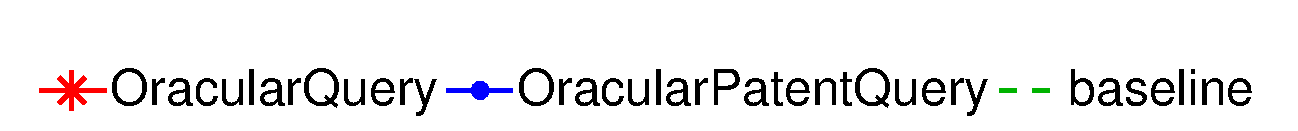
\includegraphics[width=9cm]{imgs/l1}
\par\end{centering}

\begin{centering}
\subfigure[{}\label{fig:lang-a}]{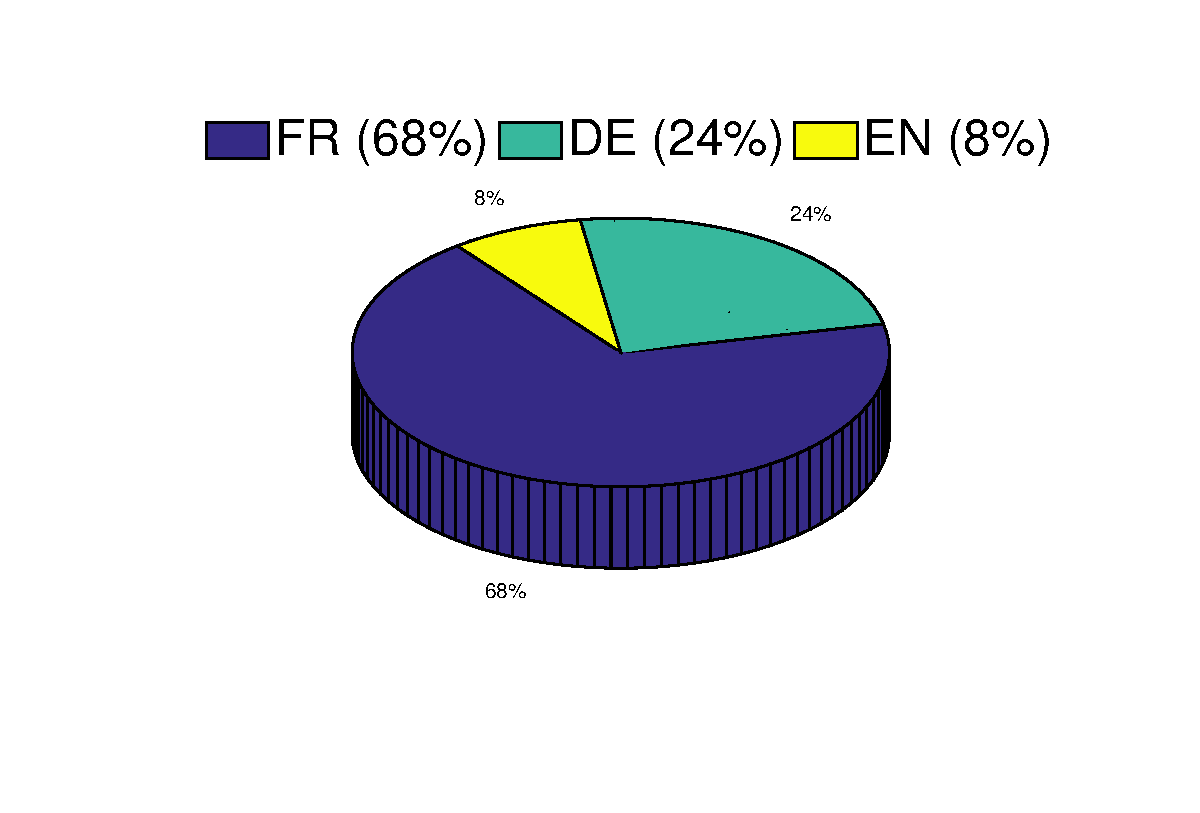
\includegraphics[width=8cm]{figs/lang1.eps}}\subfigure[\label{fig:lang-b}]{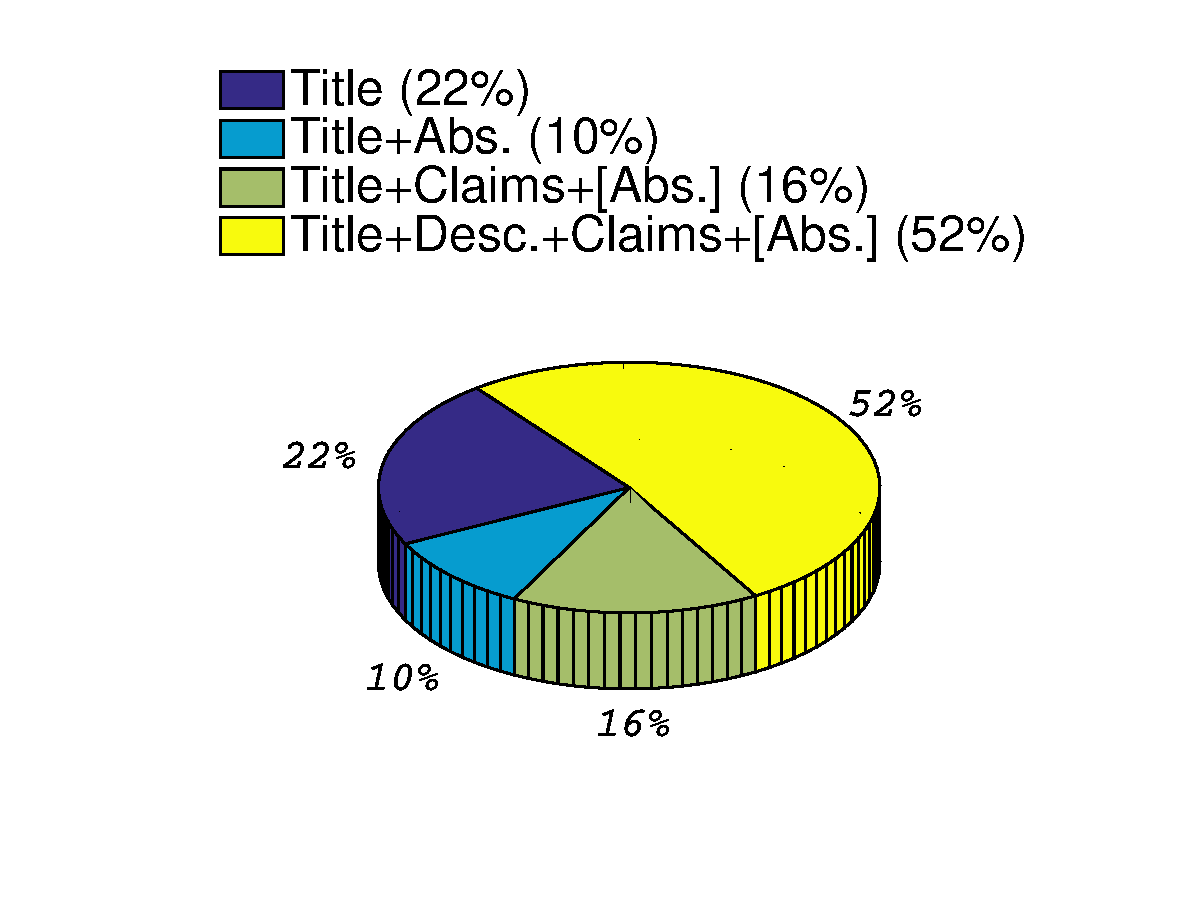
\includegraphics[width=8cm]{figs/lang2.eps}}
\par\end{centering}
\vspace{1mm}
\protect\caption{(a) Percentage of English, German, and French patents in CLEF-IP 2010 collection.
                 (b) Completeness of the presence of English text in the CLEF-IP 2010 patent collection.~\citep{magdy2012toward}.}
\label{fig:lang}
\end{figure}
%%%%%%%%%%%%%%%%%%%%%%%%%%%%%%%%%%%%%%%%%%%%%%%%%%%%%%%%%%%%%%
%\begin{figure}[t!]
%\begin{centering}
%\subfigure[\label{fig:lang-a}]{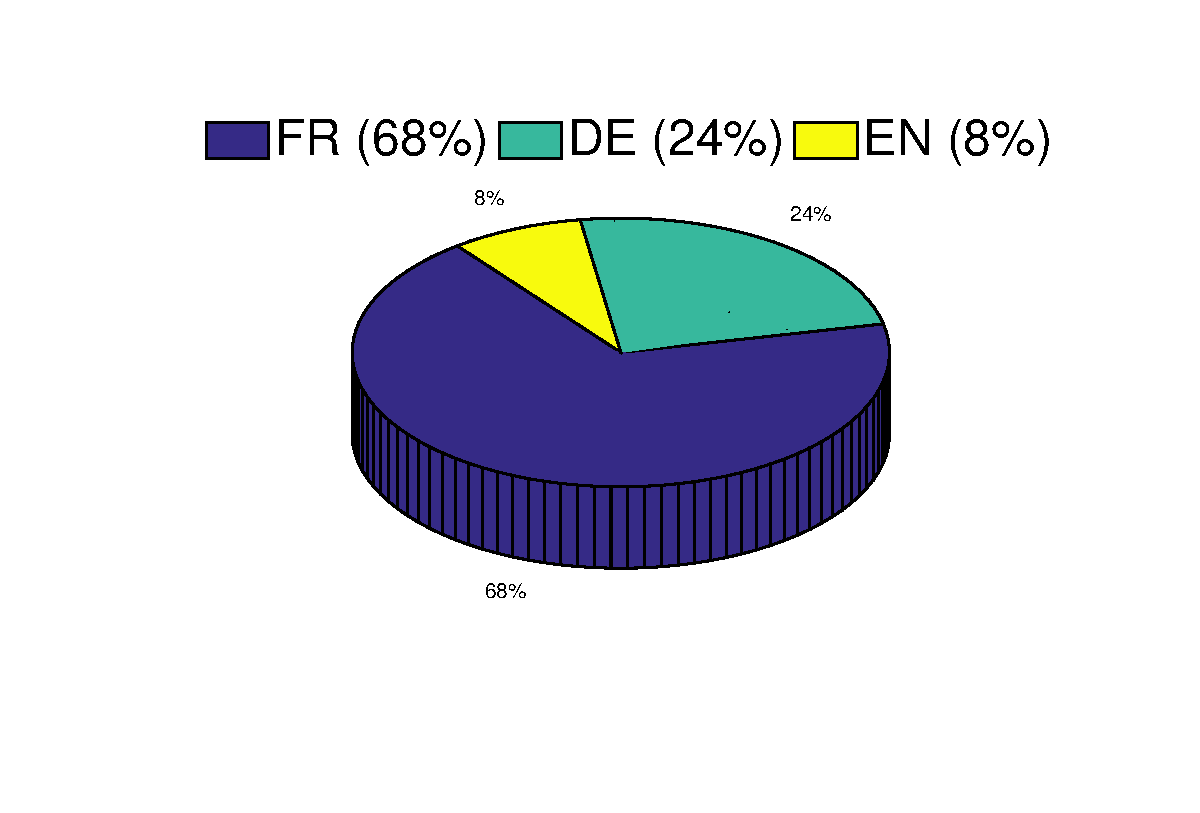
\includegraphics[width=4cm]{figs/lang1.eps}} \hspace*{1.5cm} 
%\subfigure[\label{fig:lang-b}]{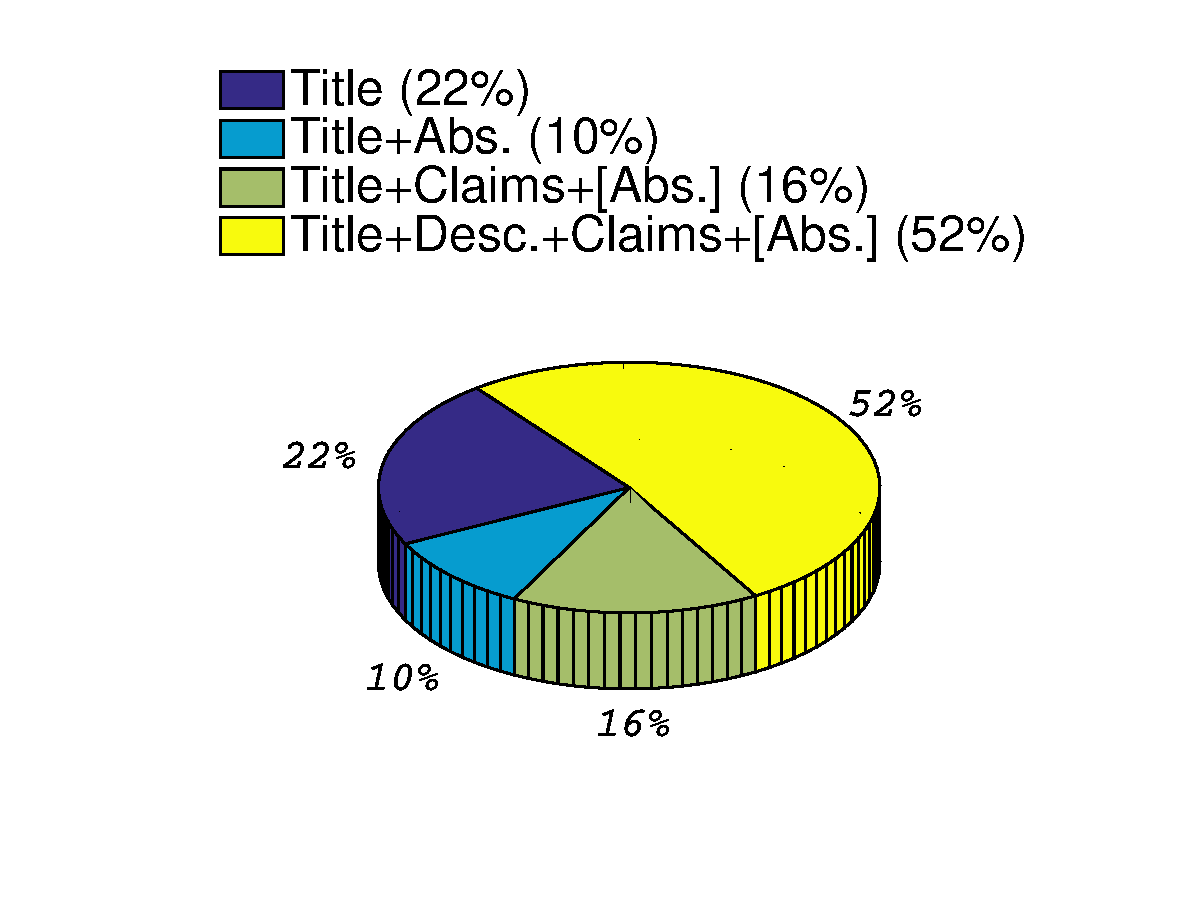
\includegraphics[width=6.5cm]{figs/lang2.eps}} 
%\par\end{centering} 
%\protect\caption{(a) Percentage of English, German, and French patents in CLEF-IP 2010 collection.
%                (b) Completeness of the presence of English text in the CLEF-IP 2010 patent collection.~\citep{magdy2012toward}}
%\label{fig:lang}
%\end{figure}

%%%%%%%%%%%%%%%%%%%%%%%%%%%%%%%%%%%%%%%%%%%%%%%%%%%%%%%%%%%%%%%%
%%%%%%%%%%%%%%%%%%%%%%%%%% Section 3 %%%%%%%%%%%%%%%%%%%%%%%%%%%
%%%%%%%%%%%%%%%%%%%%%%%%%%%%%%%%%%%%%%%%%%%%%%%%%%%%%%%%%%%%%%%%
\section{Errors Caused by Baseline Settings}
Data curation and IPC filter used in baseline settings are two sources of errors;
in this section, we will discuss these two origins of the errors.

\subsection{Data Curation Errors}
\label{sec:DataCurationErrors}
%\vspace{-2mm} 
%CLEF-IP collection has two main characteristics that leads in two main causes of the error: 
Our baseline system cannot retrieve some relevant patent documents because of two main characteristic of CLEF-IP data collection: 
\begin{enumerate}

\item \textbf{Missing description: } As we described in Section~\ref{sec:DataCollection}, some patents in the union collection lose the contents of some sections due to merging different versions of patents. Therefore, relevant patents with missing description are not retrieved by our system.
\item \textbf{Non-English relevant patents: } CLEF-IP data collection has been designed for a multilingual patent search and it consists of patents in three different languages: English, German, and French. However, our baseline $\mathit{IR}$ system is not designed for multilingual search and it cannot retrieve non-English relevant patents.   
\end{enumerate}
%%%%%%%%%%%%%%%%%%%%%%%%%%%%%%%%%%%%%%%%%%%%%%%%%%%%%%%%%%%%%%
\begin{figure}[t!]
\begin{centering}
\subfigure[Cut-off rank ($k$) $= 100$\label{fig:datacuration_a}]{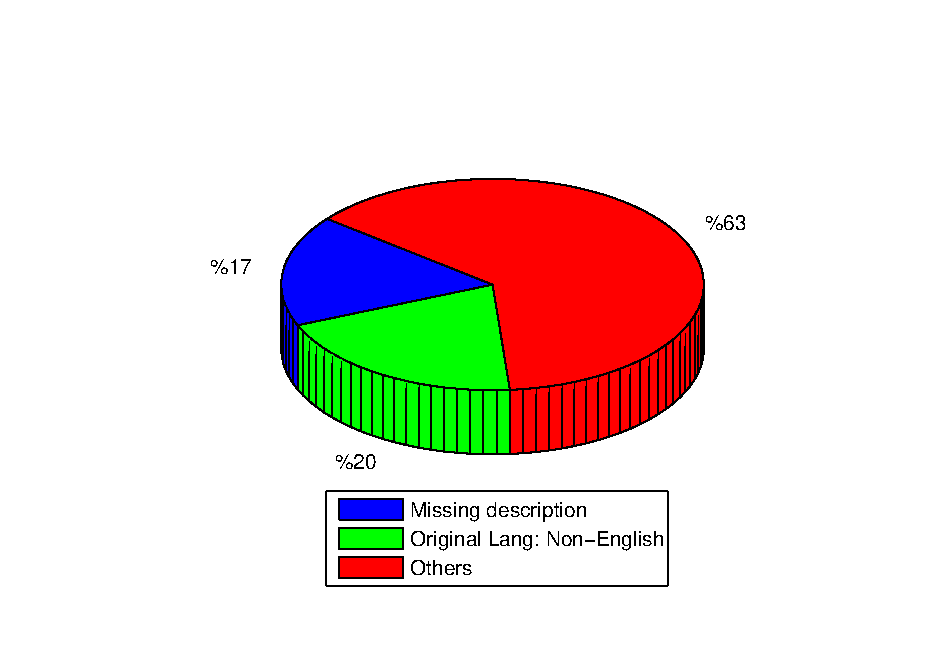
\includegraphics[width=6.5cm]{figs/analyseFNs100.eps}}  
\subfigure[Cut-off rank ($k$) $= 1,000$\label{fig:datacuration_b}]{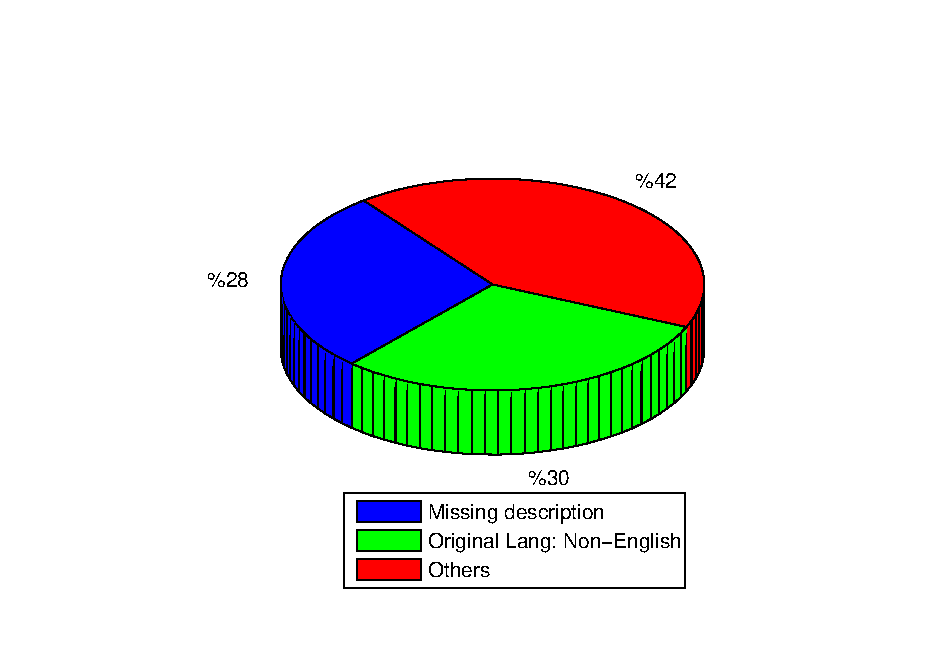
\includegraphics[width=6.5cm]{figs/analyseFNs1000.eps}} 
\par\end{centering} 
\protect\caption{Average percentage of errors due to missing description, language. Overall, $37\%$ of errors are because of data curation while $63\%$ of English complete patent documents cannot be retrieved. Increasing $k$ from $100$ to $1,000$ reduces the errors of the yellow area, but the value of $42\%$ is still notable.}
\label{fig:datacuration}
\end{figure}
%%%%%%%%%%%%%%%%%%%%%%%%%%%%%%%%%%%%%%%%%%%%%%%%%%%%%%%%%%%%%%
We calculate the percentage of errors caused by data curation in this experiment. As it has been illustrated in Figure \ref{fig:datacuration_a}
, overall, $37\%$ of errors are due to CLEF-IP data curation (missing description and non-English relevant patents) while the majority of relevant patents, which are not retrieved ($63\%$), are full English patent documents (Figure \ref{fig:datacuration}). These results indicates that the baseline retrieval system is ineffective to retrieve the majority of the relevant patents because of other reasons. In this research, we are interested in the other reasons that result in low effectiveness of general IR techniques in patent domain. Figure \ref{fig:datacuration_b} shows that by increasing the cut-off rank to $1,000$, still considerable percentage of full English relevant patents --- about $42\%$ --- are not retrieved.








%In this section, we focus on analysing not retrieved relevant (False Negative (FN)) patents. 
%%\vspace{-2mm} 
%CLEF-IP collection has two main characteristics that leads in two main causes of the error: 
%\begin{enumerate}
%\item \textit{Missing `Description': } Each patent in the collection consisted of multiple versions of documents in XML format labelled as $ A_{1} $, $ A_{2} $ ... $ B_{1} $, and $ B_{2} $. The letter `A' refers to different versions of patent applications. The `B' versions refer to granted patents. We merged different versions of a single patent into one union document as recommended by CLEF-IP%
%\footnote{\texttt{\url{http://www.ifs.tuwien.ac.at/~clef-ip/}}%
%}~\citep{magdy2012toward}. As a result of the merging, some patents in the union collection appears with many missing content fields. Since the `Description' is the longest section in a patent, almost, relevant patent with missing `Description' are not retrieved by the baseline.
%\item \textit{Non-English Patents: } The CLEF-IP has been designed for a multilingual patent search and it consists of patents in three different languages: English, German, and French. All patents have the title in the three languages while just the granted published version of a patent(`B' version) by the EPO should contain the claims section manually translated into all three languages. The description section of all patents is always in the original submission language only. Since the design of the baseline did not consider multilinguality, it can not retrieve relevant but non-English patents.   
%\end{enumerate}
%\noindent Fig.(\ref{fig:datacuration}) shows that, overall, \%37 of errors are due to CLEF-IP collection while \%63 of the errors occurs for full English patent documents.
%%\vspace*{-1ex}
%%\vspace{-3.5mm} 
%%%%%%%%%%%%%%%%%%%%%%%%%%%%%%%%%%%%%%%%%%%%%%%%%%%%%%%%%%%%%%%
%\begin{figure}[t!]
%\begin{centering}
%\subfigure[Cut-off rank(k) = 100\label{fig:datacuration_a}]{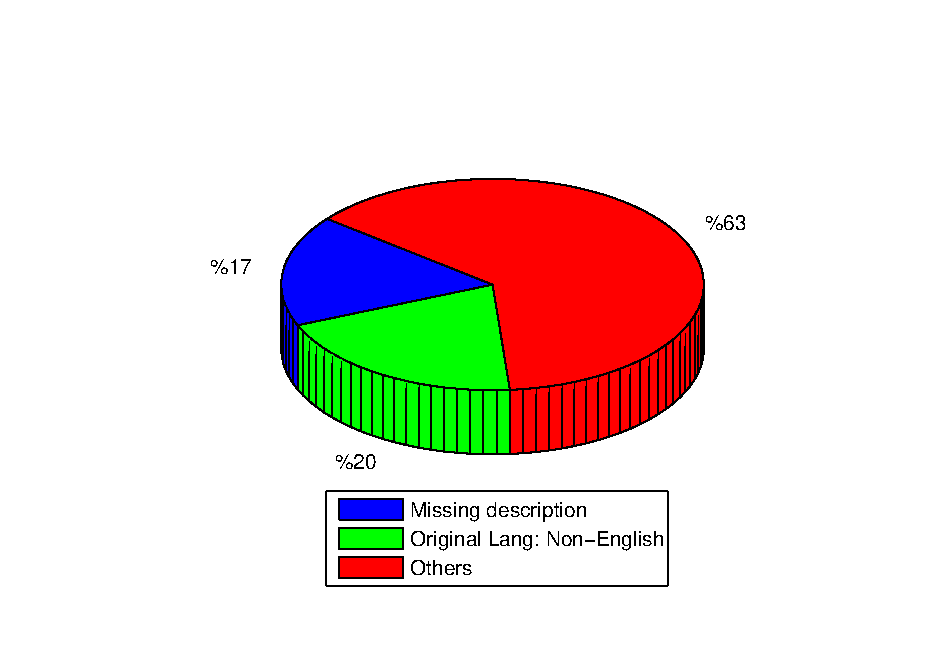
\includegraphics[width=6.5cm]{figs/analyseFNs100.eps}} \hspace*{0.5cm} 
%\subfigure[Cut-off rank(k) = 1000\label{fig:datacuration_b}]{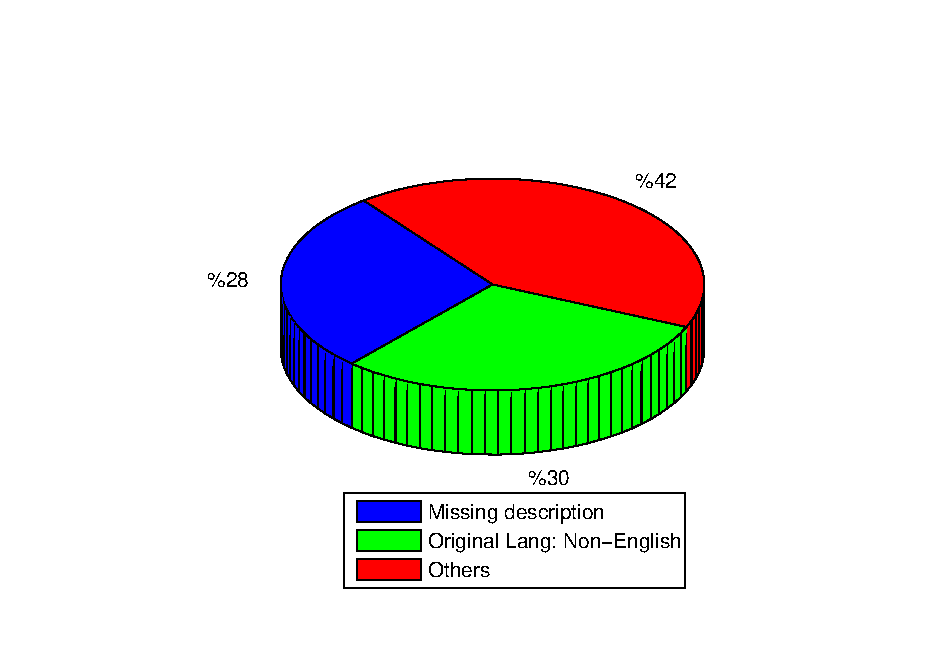
\includegraphics[width=6.5cm]{figs/analyseFNs1000.eps}} 
%\par\end{centering} 
%\protect\caption{Average percentage of errors due to missing `Description', non-English original language. Overall, 37\% of errors are because of data curation while \%63 of English complete patent documents can not be retrieved. Increasing k from 100 to 1000 reduces the errors of red area, but 42\% is still notable.}
%\label{fig:datacuration}
%\end{figure}
%%%%%%%%%%%%%%%%%%%%%%%%%%%%%%%%%%%%%%%%%%%%%%%%%%%%%%%%%%%%%%%
%%\begin{figure}[htpb]
%%%\vspace{2.5cm}
%%\centering
%%\begin{subfigure}[htpb]{.5\linewidth}
%%\centering
%%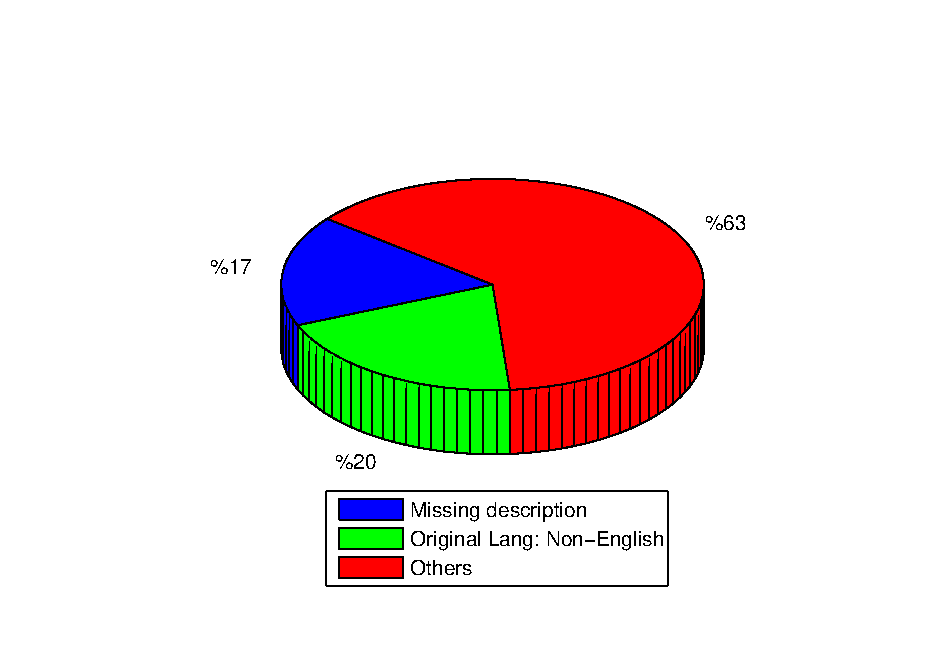
\includegraphics[width=1\textwidth,height=45mm]{figs/analyseFNs100.eps}
%%\caption{Cut-off rank(k) = 100}
%%\label{fig:datacurationk100}
%%\end{subfigure}%\\[1ex]%
%%\begin{subfigure}[htpb]{.5\linewidth}
%%\centering
%%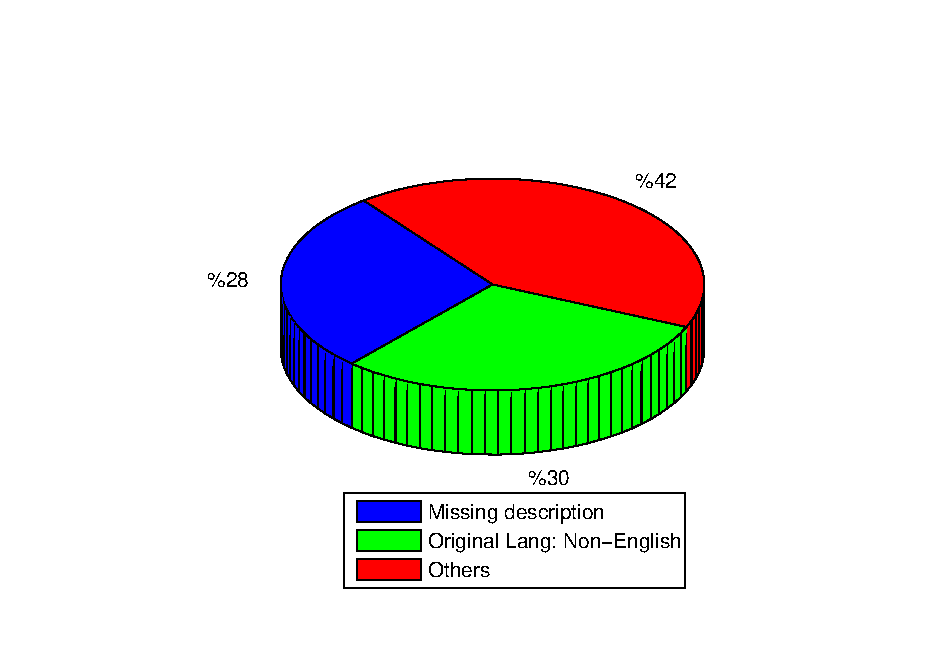
\includegraphics[width=1\textwidth,height=45mm]{figs/analyseFNs1000.eps}
%%\caption{Cut-off rank(k) = 1000}
%%\label{fig:datacurationk100}
%%\end{subfigure}
%%\caption{Average percentage of errors due to missing `Description', non-English original language. Overall, \%37 of errors are because of data curation while \%63 of English complete patent documents can not be retrieved. Increasing k from 100 to 1000 reduces the errors of red area, but \%42 is still notable.}
%%\label{fig:datacuration}
%%\end{figure}
%%\FloatBarrier
%%\noindent
%
%%Table \ref{tab:FNs} compares the average percentage of relevant patents which are not retrieved at top 100, 200, and 1000. 
%%\begin{table*}[htpb]
%%  \begin{center}
%%  \input table/FNs.tex  
%%  \caption{The percentage of relevant documents which are not retrieved at top 100, k= 100, over all test queries. In average, \%57 of relevant patents can not be retrieved by the system at top 100.}
%%  \label{tab:FNs}
%%  \end{center}  
%%\end{table*}
%%\FloatBarrier 
%%\noindent
%
%
%%We categorised the source of failure in three groups:
%%\begin{enumerate}
%%\item patents with missing description.
%%\item patents with non-English original language.
%%\item others: patents which are complete and their original language is English. The reason that they are not retrieved is still unknown, but our hypothesis is that these patents can not be retrieved because they have less term overlap with their related query. 
%%%containing the least term overlap with the query.
%%\end{enumerate}
%%The two first groups are the characteristic of our collection and we are not interested in improve the baseline to retrieve them. Whereas, we are interested in improve our system to be able to retrieve the third group.
%%Figure \ref{fig:failingCategory} shows the percentage of each failure source averaged over all queries in FN subset (k = 100).
%%\begin{figure}[htpb]
%%   \centering
%%   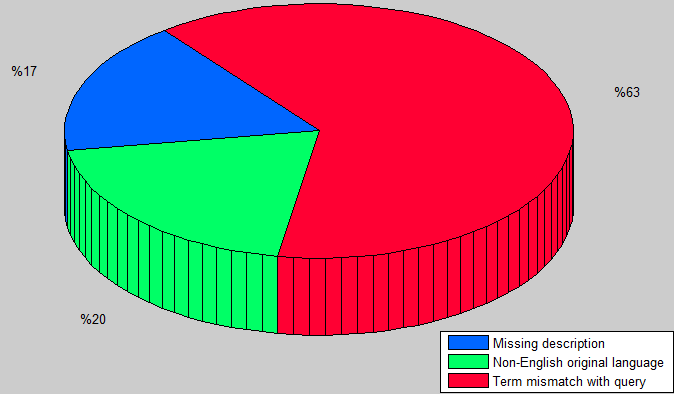
\includegraphics[width=0.55\textwidth,height=45mm]{figs/failingCategory.png}
%%   \caption{Average percentage of patents with missing description, non-English original language, and term mismatch with the query in FN patents over all queries.(k=100).}  
%%   \label{fig:failingCategory} 
%%\end{figure}
%%\FloatBarrier 
%%\noindent
%
%By increasing the ranking threshold to 1000, the percentage of term mismatch failure source decreases in FN subset; Whereas, \%41 is still considerable. 
%
%%\begin{figure}[htpb]
%%   \centering
%%   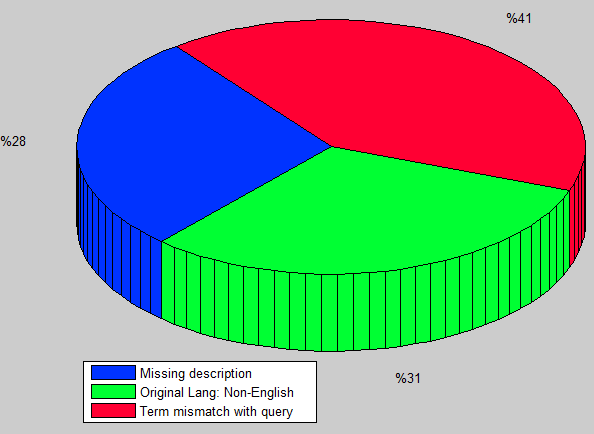
\includegraphics[width=0.55\textwidth,height=55mm]{figs/FNs-k1000.png}
%%   \caption{Average percentage of patents with missing description, non-English original language, and term mismatch with the query in FN patents over all queries.(k=1000).}  
%%   \label{fig:FNs-k1000} 
%%\end{figure}
%%\FloatBarrier 
%%\noindent
%
%We can conclude from Fig. \ref{fig:datacuration} that the main reason, which relevant documents are not retrieved, is the term mismatch between the query and relevant patents,  even in top 1000 documents. The portion of missing description and non-English original language are also high enough to deteriorate the system performance. In our research, we focus on term mismatch between query and relevant documents not missing description or multilinguality which are specific to clef-ip data collection.
%
%Our detailed results also indicate that by increasing the ranking threshold from 100 to 1000, the number of false negatives due to term mismatch between query and relevant documents decreased. Whereas there are some queries that their relevant patents in English do not retrieve even at the rank 1000. 
%
%The focus of this research is to identify the reasons that the system fails to retrieve patents in the red area, where the patents are complete English documents. Hence, in the rest of this paper, we continue our experiment in the red area.\\\\
%\textbf{Anecdotal Examples}\\
%In following experiments, we selected five sample queries from the category: "other"; The following figures show the query term frequency in relevant not-retrieved patents. 
%\begin{landscape}
%\begin{figure}[htpb]
%   \centering
%   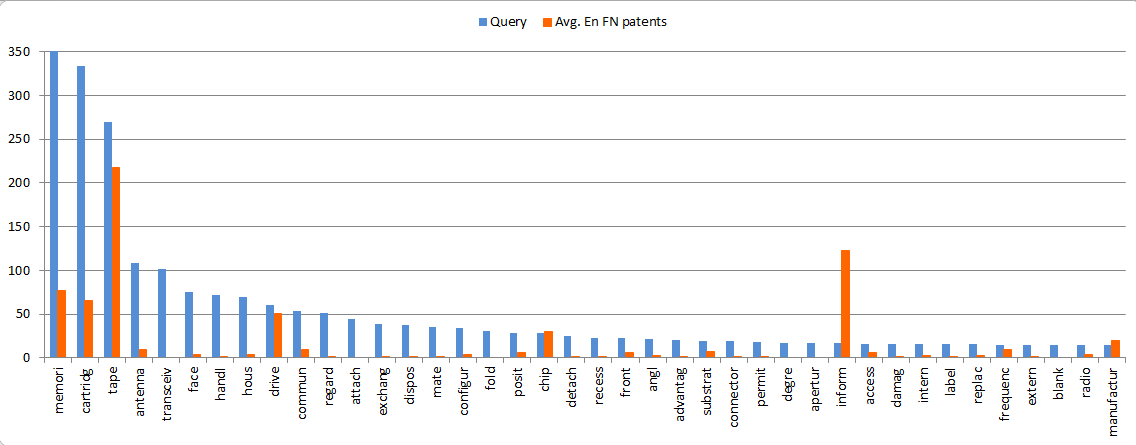
\includegraphics[width=\columnwidth,height=100mm]{figs/pac1035-avgEnFNs.png}
%   \caption{Comparing term frequencies in query, and average term frequencies in relevant not-retrieved patents for Query: PAC-1035. 6/8 patents which are also English can not be retrieved before rank 100, but all can be retrieved before the rank 1000. This indicates that although there is few overlap between query and relevant patents, they will be retrieved but at higher ranks after 100.} 
%   \label{fig:fn-pac1035} 
%\end{figure}
%\end{landscape}
%\FloatBarrier
%\noindent
%  
%\begin{landscape}
%\begin{figure}[htpb]
%   \centering
%   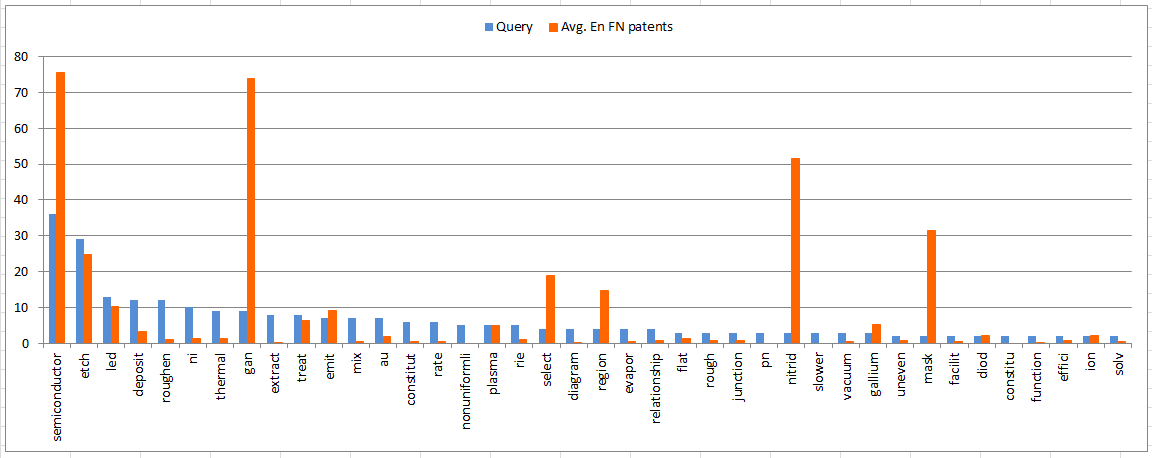
\includegraphics[width=\columnwidth,height=100mm]{figs/fn-pac1142.png}
%   \caption{Comparing term frequencies in query, and average term frequencies in relevant not-retrieved patents for Query: PAC-1142. (En FNs)/FNs = 9/10, @ k=100, and still (En FNs)/FNs = 7/10 @ k=1000. This indicates that 7 relevant patents for this query are not retrievable.} 
%   \label{fig:fn-pac1142} 
%\end{figure}
%\end{landscape}
%\FloatBarrier
%\noindent
%
%\begin{landscape}
%\begin{figure}[htpb]
%   \centering
%   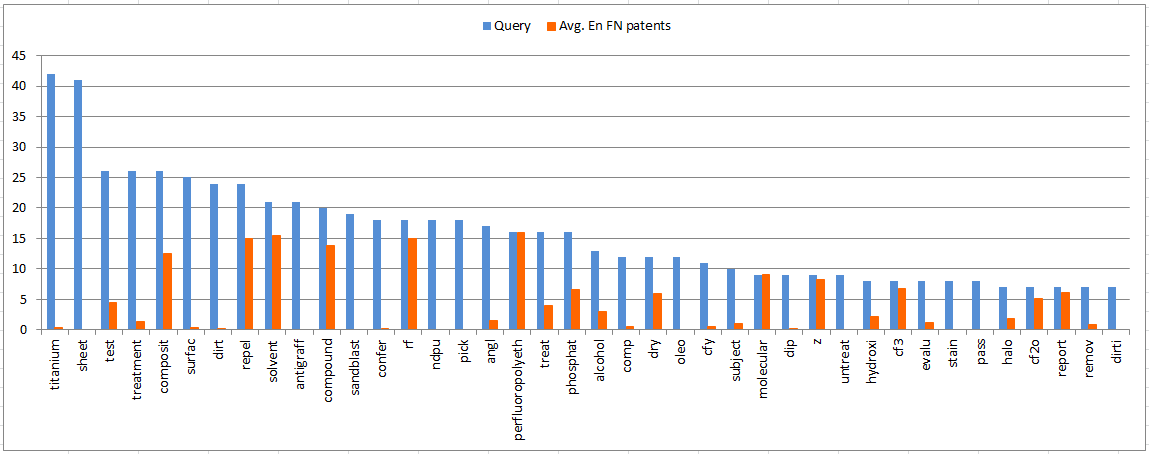
\includegraphics[width=\columnwidth,height=100mm]{figs/fn-pac1216.png}
%   \caption{Comparing term frequencies in query, and average term frequencies in relevant not-retrieved patents for Query: PAC-1216. This query is an example that its English relevant patents (5/6) can not be retrieved even at rank 1000.} 
%   \label{fig:fn-pac1216} 
%\end{figure}
%\end{landscape}
%\FloatBarrier
%\noindent
%
%\begin{landscape}
%\begin{figure}[htpb]
%   \centering
%   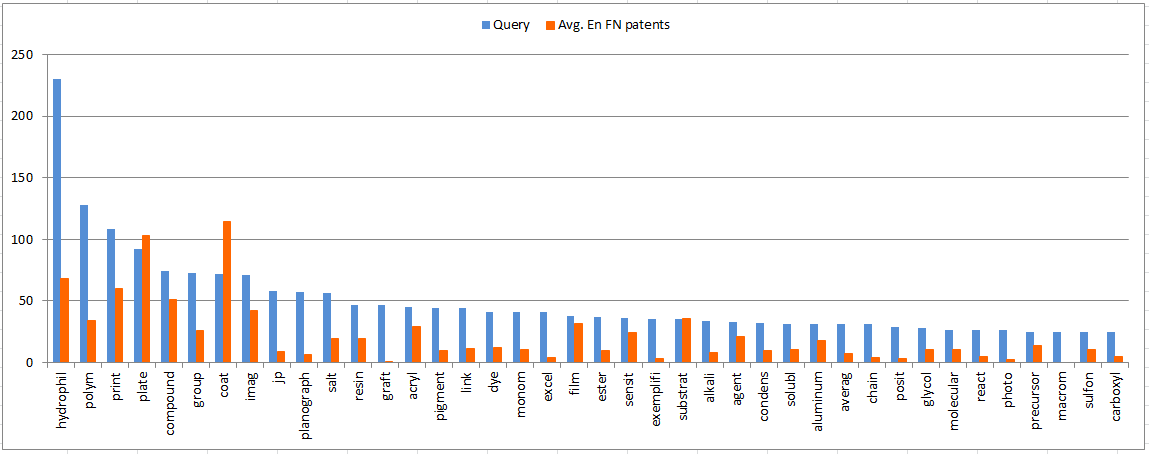
\includegraphics[width=\columnwidth,height=100mm]{figs/fn-pac1379.png}
%   \caption{Comparing term frequencies in query, and average term frequencies in relevant not-retrieved patents for Query: PAC-1379. (En FNs)/FNs = 14/17, @ k=100, and still (En FNs)/FNs = 12/17, @ k=1000. This indicates that 12 English relevant patents for this query are not retrievable.} 
%   \label{fig:fn-pac1379} 
%\end{figure}
%\end{landscape}
%\FloatBarrier
%\noindent
%
%\begin{landscape}
%\begin{figure}[htpb]
%   \centering
%   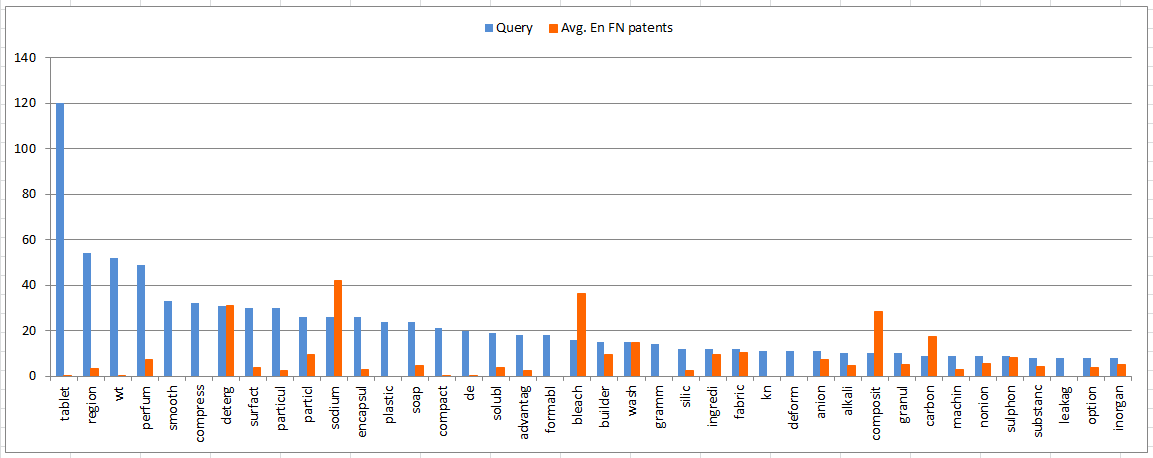
\includegraphics[width=\columnwidth,height=100mm]{figs/fn-pac1604.png}
%   \caption{Comparing term frequencies in query, and average term frequencies in relevant not-retrieved patents for Query: PAC-1604. (En FNs)/FNs = 10/19, @ k=100, and still (En FNs)/FNs = 9/19 @ k=1000. This indicates that 9 English relevant patents for this query are not retrievable.} 
%   \label{fig:fn-pac1604} 
%\end{figure}
%\end{landscape}
%\FloatBarrier
%\noindent
%Our experiments showed the reason that some relevant patents are not retrieved by the system is not that there is zero term overlap between the query and documents, it is low weighting of query terms in the relevant documents. 



%\begin{table*}[htpb]
%  \begin{center}
%  \input table/errorCategory.tex  
%  \caption{Percentage of missing, non-English, and term mismatch error category in FN patents. }
%  \label{tab:threshold}
%  \end{center}  
%\end{table*}
%\FloatBarrier 
%\noindent

%Patent retrieval is a recall-oriented task and it is important to retrieve all relevant patents appear at top of the list. Patent examiners, our users, usually prefer to look at 100-200 top retrieved patents. Table \ref{tab:threshold} shows about \%16 decrease in recall which are not desired for our users. 
%\begin{table*}[htpb]
%  \begin{center}
%  \input table/threshold.tex  
%  \caption{Comparing performance of the baseline by changing the retrieval threshold.}
%  \label{tab:threshold}
%  \end{center}  
%\end{table*}
%\FloatBarrier 
%\noindent
%
%\begin{figure}[htpb]
%   \centering
%   \includegraphics[width=0.65\textwidth,height=65mm]{figs/a1000.png}
%   \caption{Baseline performance variation over all queries (k=1000).}  
%   \label{fig:a1000} 
%\end{figure}
%\FloatBarrier 
%\noindent
%%
%%\begin{figure}[htpb]
%%   \centering
%%   \includegraphics[width=0.65\textwidth,height=65mm]{figs/a100.png}
%%   \caption{Baseline performance variation over all queries (k=100).}  
%%   \label{fig:a100} 
%%\end{figure}
%%\FloatBarrier 
%%\noindent
%
%\begin{figure}[htpb]
%\label{fig:base}
%        \centering
%        \begin{subfigure}[b]{0.6\textwidth}
%        \centering
%                \includegraphics[width=1\textwidth,height=65mm]{figs/a100.png}
%                \caption{ }
%                \label{fig:baseperformancea}
%        \end{subfigure}%
%        ~ %add desired spacing between images, e. g. ~, \quad, \qquad, \hfill etc.
%          %(or a blank line to force the subfigure onto a new line)
%        \begin{subfigure}[b]{0.6\textwidth}
%        \centering
%                \includegraphics[width=1\textwidth,height=65mm]{figs/a1000.png}
%                \caption{ }
%                \label{fig:baseperformanceb}
%        \end{subfigure}
%       \caption{
%                Baseline performance variation over all queries (a) k=1000.
%                (b) k=100.
%                } 
%\end{figure}
%\FloatBarrier
%\noindent
%Figure \ref{fig:baseperformancea} and \ref{fig:baseperformanceb} show the variation of the baseline system performance. Figure \ref{fig:baseperformancea} is when choosing the top rank k = 100 and figure \ref{fig:baseperformanceb} is for k = 1000. It can be seen that 'Recall' and 'PRES' skew up when we increase the rank threshold, but there is no significant improvement for 'Average Precision (AP)' because it is more sensitive to finding relevant documents at very high ranks regardless of the number of documents to be checked by the user. However, 'PRES' is more sensitive to the average ranking of the relevant retrieved documents as a whole relative to the maximum number of documents the user is willing to check. Foe example, when Nmax=1000, the ranks {32, 35, 46} are considered relatively good compared to this number. Nevertheless, when calculating PRES with Nmax=100, the PRES value will be less which represents the average ranking of the relevant documents relative to the maximum number of documents to be checked. Low 'AP' indicates that system is also incapable of retrieving patents at top of the list with high ranks. The reason was indicated in previous section (term level analysis), irrelevant patents have more common words with the query which ends in retrieving them at top of the list. The solution is finding the noisy words which appear more in the irrelevant documents and should be identified and removed. 
%%\begin{list}{-}{}
%%\end{list}


%%%%%%%%%%%%%%%%%%%%%%%%%%%%%%%%%%%%%%%%%%%%%%%%%%%%%%%%%%%%%%%%
\subsection{Classification Code Mismatch}
\label{sec:ClassificationCodeMismatch}

%\subsubsection{International Patent Classification code}
%In 1971, the Strasbourg Agreement established the International Patent Classification (IPC) under the World Intellectual Property Organization (WIPO), which divides technology into eight discrete Sections. The goal of this
%Agreement was to overcome the difficulties caused by using diverse national patent classification systems.~\citep{harris2010comparison}
%
%A patent is assigned to one or more of the 71,000 IPC codes that 
%indicate the related technical field or fields the patent covers. 
%These codes are arranged in a hierarchical, tree-like structure with 
%five distinct components. Fig. \ref{fig:ipcexample} illustrates the components of an IPC classification.
%
%The highest hierarchical level contains the eight sections of the IPC corresponding
%to very broad technical fields, labeled A through H. For example, Section C deals
%with``Chemistry and Metallurgy''. Sections are subdivided into classes. The eighth edition of the IPC contains 120
%classes. Class C07, for example, deals with ``Organic Chemistry''. Classes are further subdivided into more than 600 subclasses. Subclass C07C, for example, deals with ``Acyclic or Carbocyclic Compounds''. Subclasses are then further divided into main groups and subgroups. Main group symbols end with ``/00''. Ten percent of all IPC groups are main
%groups. For example, main group C07C 35/00 deals with ``Compounds having at
%least one hydroxy or O-metal group bound to a carbon atom of a ring other than
%a six-membered aromatic ring''. In some versions of the IPC, a series of numbers will follow the subgroup, reflecting
%the enactment date of the IPC version. `20060101' following the Subgroup
%indicates a date of January 1, 2006, which is the date that the eighth version of
%the IPC took effect. 
%%%%%%%%%%%%%%%%%%%%%%%%%%%%%%%%%%%%%%%%%%%%%%%%%%%%%%%%%%%%%%%%%%%%%%%%%%%%%%%%%%
%\begin{figure}[t!]
%   \centering
%   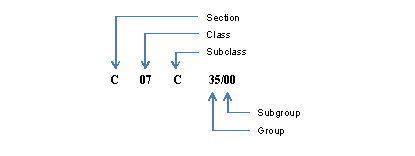
\includegraphics[width=0.70\textwidth,height=35mm]{figs/IPCexample.jpg}
%   \caption{An example illustrating the components of an International Patent Classification code.}   
%   \label{fig:ipcexample} 
%\end{figure}
%%%%%%%%%%%%%%%%%%%%%%%%%%%%%%%%%%%%%%%%%%%%%%%%%%%%%%%%%%%%%%%%%%%%%%%%%%%%%%%%%%
%\subsubsection{IPC Classification as a Filter}
As we mentioned in Section~\ref{sec:settings}, IPC codes (Section~\ref{StructureofPatents}) 
are assigned to patent queries to filter the search results by constraining them to have common IPC codes with the patent query.
In this section, we investigate the errors caused by classification code mismatch between topics (queries) and relevant documents for three different level of hierarchy. 
 
%\subsubsection{Applying 4-digit IPC code for filtering}
%\label{subsec: 4-digit}
\paragraph{Filter Type I: Three First Components of IPC Code}
\ \\
First, we examine the effect of filtering out the patents, which their three first symbols of IPC code, including section, class, and subclass (e.g., $\mathit{C07C}$ in Figure~\ref{fig:ipcexample}), do not match with the patent query. We have applied this filter to our baseline system. As a consequence, relevant patents, which do not share these three symbols of the IPC code with the patent query, are not retrieved by the system.   

Our experiments show that   
around 19\% of the not-retrieved relevant patents do not share any IPC code with the patent query, but the majority of them have main IPC code of the query, and about 21\% have, at least, one of the further IPC codes of the query (Figure~\ref{fig:ipcoverlap_a}). 
%%%%%%%%%%%%%%%%%%%%%%%%%%%%%%%%%%%%%%%%%%%%%%%%%%%%%%%%%%%%%%%%%%%%%%%%%%%%%%%%%
%\begin{figure}[t!]
%   \centering
%   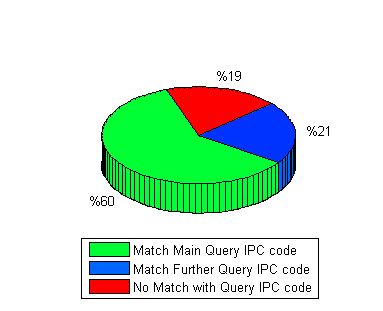
\includegraphics[width=0.60\textwidth,height=69mm]{figs/ipcOverlap-FNs.png}
%   \caption{Classification code overlap between the query and non-relevant retrieved patents (False Negative (FN) patents).}   
%   \label{fig:fnipcoverlap} 
%\end{figure}
%%%%%%%%%%%%%%%%%%%%%%%%%%%%%%%%%%%%%%%%%%%%%%%%%%%%%%%%%%%%%%%%%%%%%%%%%%%%%%%%%
%%%%%%%%%%%%%%%%%%%%%%%%%%%%%%%%%%%%%%%%%%%%%%%%%%%%%%%%%%%%%%
\begin{figure}[t!]
\begin{centering}
\subfigure[Not-retrieved relevant patents (False Negative (FN) patents)\label{fig:ipcoverlap_a}]{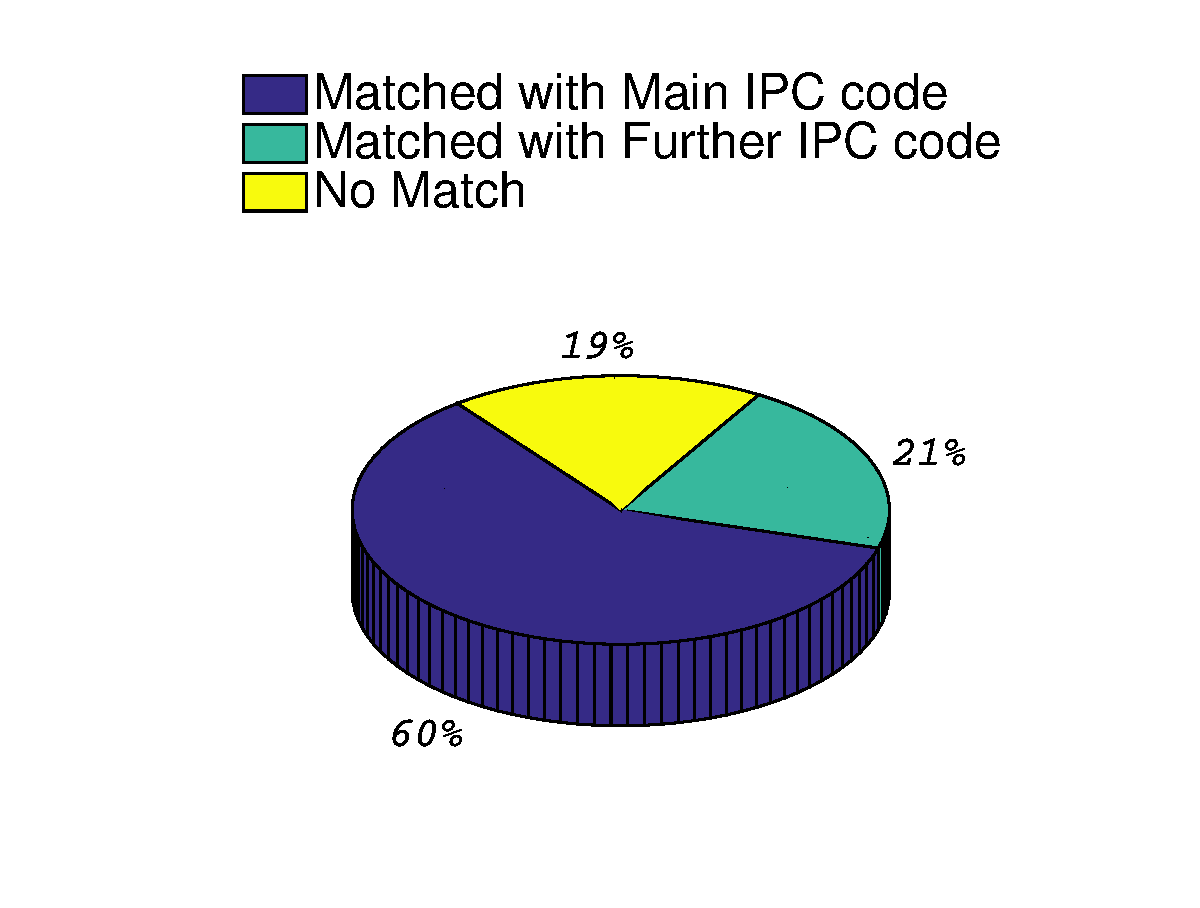
\includegraphics[width=6.5cm]{figs/ipcOverlap-FNs.eps}} 
\hspace*{0.5cm}  \subfigure[Retrieved relevant patents (True Positive (TP) patents)\label{fig:ipcoverlap_b}]{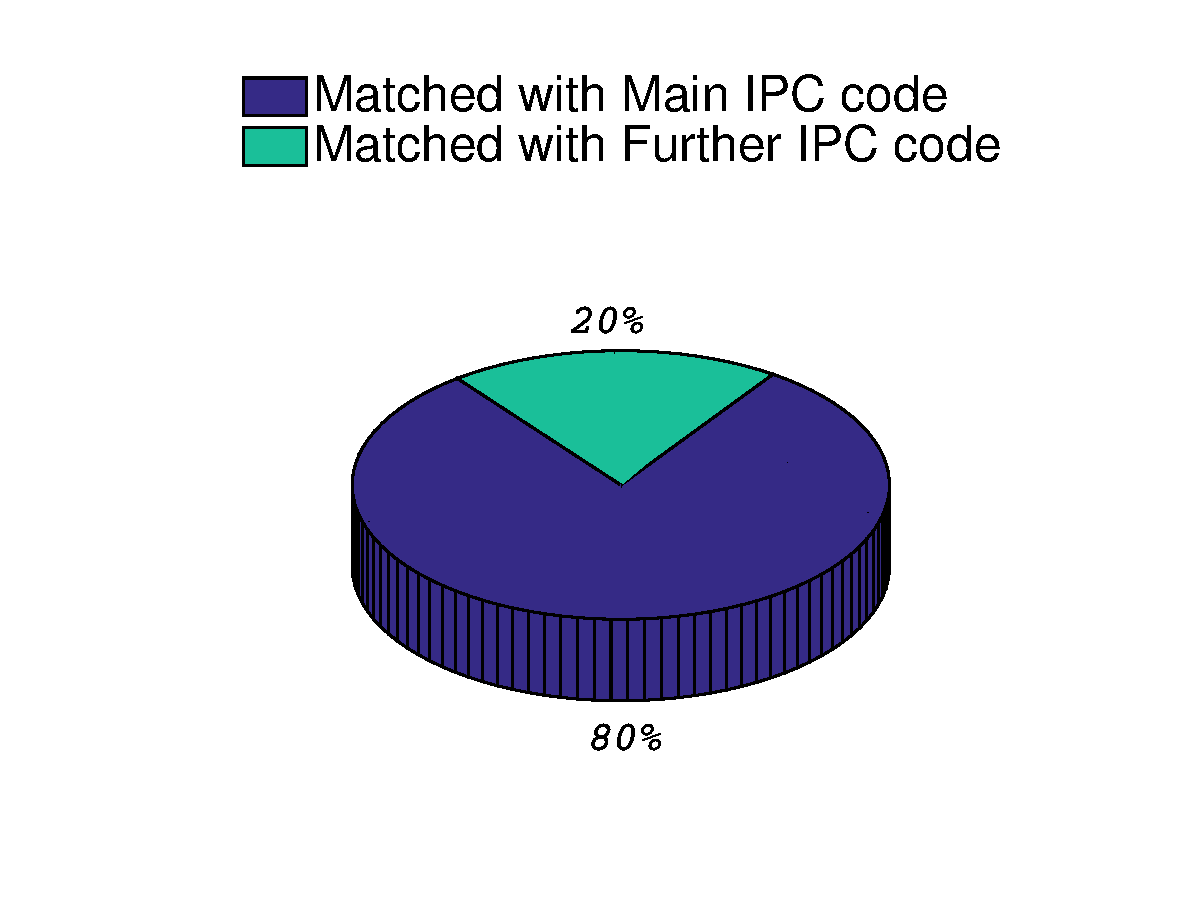
\includegraphics[width=6.5cm]{figs/ipcOverlap-TPs.eps}} 

\par\end{centering} 
\protect\caption{Classification code overlap between the query and non-relevant retrieved patents (False Negative (FN) patents).}
\label{fig:ipcoverlap}
\end{figure}
%%%%%%%%%%%%%%%%%%%%%%%%%%%%%%%%%%%%%%%%%%%%%%%%%%%%%%%%%%%%%%
We repeat the experiments for the true positive (TP) patents; as it has been shown in Figure \ref{fig:ipcoverlap_b}, 80\% of TP patents have an overlap with the main IPC code of the query and 20\% with, at least, one of the query further IPC codes. 
%So, we can conclude that 19\% of errors can be due to IPC filtering if we assume that they have enough term overlap with the query.  
%%%%%%%%%%%%%%%%%%%%%%%%%%%%%%%%%%%%%%%%%%%%%%%%%%%%%%%%%%%%%%%%%%%%%%%%%%%%%%%%%
%\begin{figure}[t!]
%   \centering
%   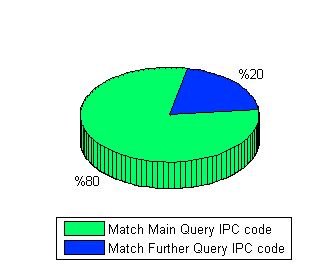
\includegraphics[width=0.55\textwidth,height=60mm]{figs/ipcOverlap-TPs.png}
%   \caption{Classification code overlap between the query and relevant retrieved patents (True Positive (TP) patents).}   
%   \label{fig:tpipcoverlap} 
%\end{figure}
%%%%%%%%%%%%%%%%%%%%%%%%%%%%%%%%%%%%%%%%%%%%%%%%%%%%%%%%%%%%%%%%%%%%%%%%%%%%%%%%%
Although we cannot retrieve around 19\% of relevant patents as a result of applying the IPC filter, we still keep using the filter in our experiments for the following two main reasons: 
\begin{enumerate}
\item CLEF-IP 2010 collection contains 2.6 million patent documents. If we do not use the IPC filter, it will take long time to compare each patent in the whole collection with the query. Nonetheless, if we apply the filter, this process will take faster because the matching process is done on only the portion of the collection, which shares an IPC code with the patent query not the whole collection. Since only less than 19\% of errors are due to a classification mismatch, we continue our analysis by keeping the filter on. The matching process is computationally much faster when we apply the IPC filter. In trade off between losing the percentage of the relevant patents and faster computation, we choose the efficient computation. The computational time is critical in patent prior art search because the query is the description of the the patent query, consisting of thousands of words.   
\item The precision in the top $k$ (100) significantly drops, when we rank the whole collection versus only a subset of patents that have the same classification code with the patent query.  
\end{enumerate}

We conduct the following experiment to justify the first above-mentioned reason. First, we calculate the number of documents that should be processed during the ranking process per query after applying the filter. Then we plot the distribution of this number over all test topics.
%%%%%%%%%%%%%%%%%%%%%%%%%%%%%%%%%%%%%%%%%%%%%%%%%%%%%%%%%%%%%%%%%%%%%%%%%%%%%%%%%
\begin{figure}[t!]
   \centering
   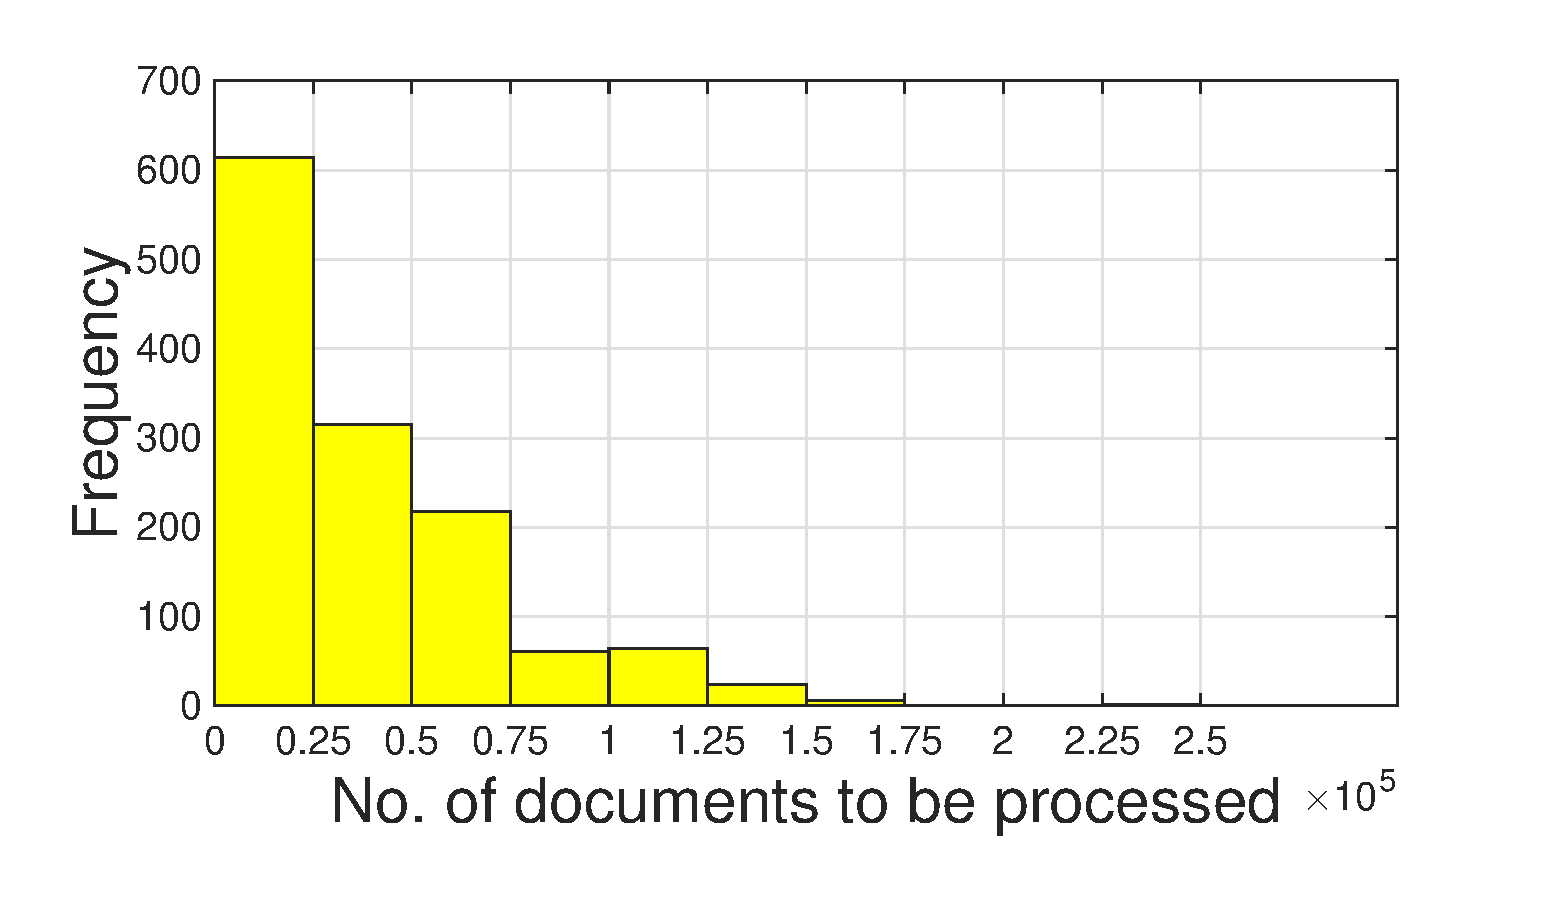
\includegraphics[width=0.70\textwidth,height=55mm]{figs/filter1}
   \caption{The distribution of the number of patents that should be ranked for each query over all test topics ($1,303$), after applying the IPC filter (filter type I).
On average, the matching process for each query is done over $ 36,254 $ documents instead of the whole collection (2.6 million documents), which dramatically reduces the computational time.}   
   \label{fig:ipcfilter-histo} 
\end{figure}
%%%%%%%%%%%%%%%%%%%%%%%%%%%%%%%%%%%%%%%%%%%%%%%%%%%%%%%%%%%%%%%%%%%%%%%%%%%%%%%%%
%\FloatBarrier 
%\noindent
Figure~\ref{fig:ipcfilter-histo} illustrates that the matching process should be only done over $25,000$ documents for the majority of queries. On average, this number is $ 36,254 $, which indicates that the system just needs to look into $ 36,254 $ documents per query on average instead of the entire collection that contains 2.6 million patent documents. Therefore, applying the IPC filter computationally saves us considerable amount of time.   

In trade off between losing 19\% of relevant patents and making the ranking process faster, we choose faster computation. In addition, we notice that the histogram falls down by increasing the number of documents that should be processed; this means that for the majority of queries the matching process is done over less number of patent documents.
%\vspace{-1cm}
%\subsubsection{Applying First two IPC code components for filtering}
%\label{subsec: Firsttwocomponents}
\paragraph{Filter Type II: Two First Components of IPC Code}
%\textbf{(B) Filter: First two components of the IPC code}
\ \\
We hypothesise that the errors will be reduced, if we broaden the filter by selecting two first components of the query IPC, namely, section, and class (e.g., C07). We repeat the experiments for filter type II.
The results have been illustrated in Figure~\ref{fig:ipc1stTwoElements}. Figure~\ref{fig:ipc1stTwoElements_a} shows that we can reduce the errors related to filtering from 19\% to 13\% by omitting the subclass component. However, the number of documents that should be ranked increases from $ 36,254 $ to $ 99,754 $ on average. As it can be seen in Figure~\ref{fig:ipc1stTwoElements_b}, the distribution of the number of documents that should be compared in matching process does not follow the falling trend as filtering with three first components. We conclude that this filter is not appropriate since we only reduce the error by 6\% whereas the average number of documents, which should be processed,~triples.    
%%%%%%%%%%%%%%%%%%%%%%%%%%%%%%%%%%%%%%%%%%%%%%%%%%%%%%%%%%%%%%%%%%%%%%%%%%%%%%%%%
%\begin{figure}[t!]
%   \centering
%   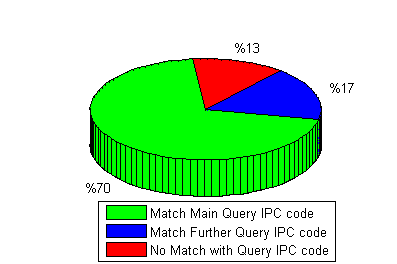
\includegraphics[width=0.55\textwidth,height=60mm]{figs/ipc1stTwoElements.png}
%   \caption{Filter: The first two components (Section and Class).}   
%   \label{fig:ipc1stTwoElements} 
%\end{figure}
%%%%%%%%%%%%%%%%%%%%%%%%%%%%%%%%%%%%%%%%%%%%%%%%%%%%%%%%%%%%%%%%%%%%%%%%%%%%%%%%%
%%%%%%%%%%%%%%%%%%%%%%%%%%%%%%%%%%%%%%%%%%%%%%%%%%%%%%%%%%%%%%
\begin{figure}[t!]
\begin{centering}
\subfigure[The portion of patents in the collection which are matched with the query IPC code. \label{fig:ipc1stTwoElements_a}]{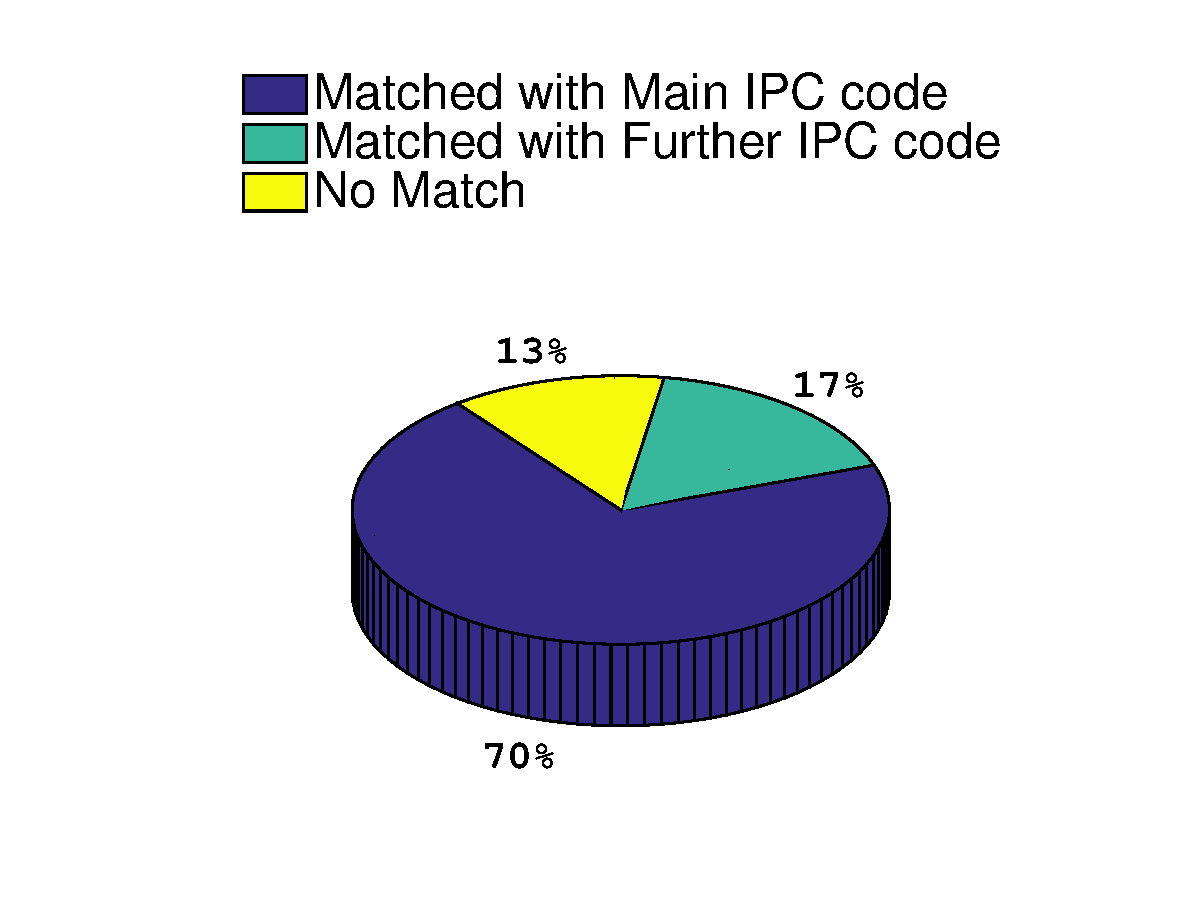
\includegraphics[width=7.5cm, height=6cm]{figs/filter2_pie}} 
\\[1ex]%
\subfigure[The distribution of the number of patents should be ranked for each query over all test queries ($1,303$).
In average, the matching process for each query is done over $ 99,754 $ documents instead of the whole collection (2.6 million documents), which dramatically reduce the computational time.\label{fig:ipc1stTwoElements_b}]{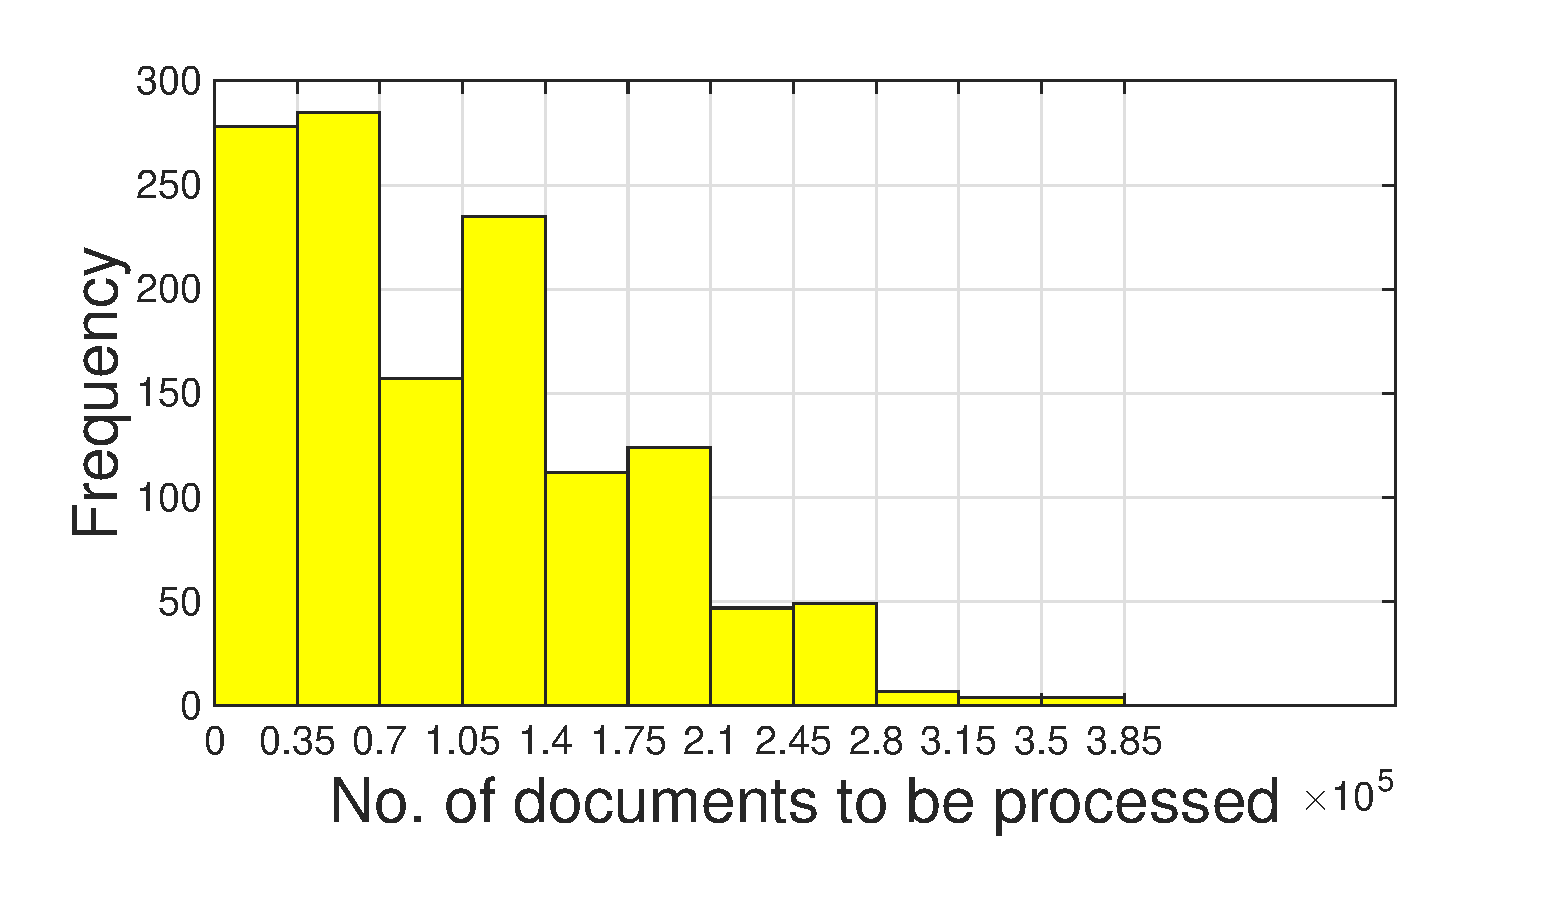
\includegraphics[width=9.5cm, height=6cm]{figs/filter2}} 

\par\end{centering} 
\protect\caption{Applying first two IPC code components (Section and Class) for filtering}
\label{fig:ipc1stTwoElements}
\end{figure}
%%%%%%%%%%%%%%%%%%%%%%%%%%%%%%%%%%%%%%%%%%%%%%%%%%%%%%%%%%%%%%
%\begin{figure}[htpb]
%\centering
%\begin{subfigure}[htpb]{.5\linewidth}
%\centering
%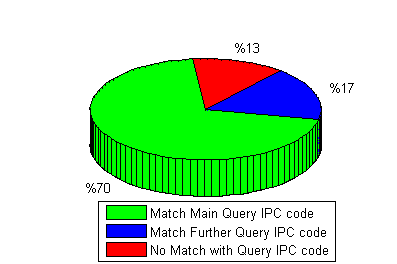
\includegraphics[width=1\textwidth,height=55mm]{figs/ipc1stTwoElements.png}
%\caption{Filter: The first two components (Section and Class)}
%\label{fig:ipc1stTwoElements}
%\end{subfigure}%\\[1ex]%
%\begin{subfigure}[htpb]{.5\linewidth}
%\centering
%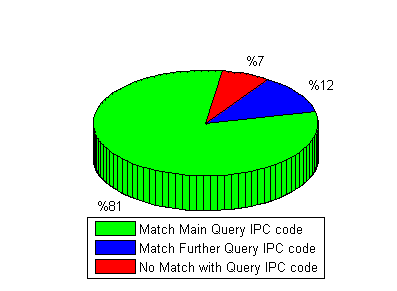
\includegraphics[width=1\textwidth,height=55mm]{figs/ipc1stElement.png}
%\caption{Filter: Only the first component (Section)}
%\label{fig:ipc1stElement}
%\end{subfigure}
%\caption{IPC classification overlap between the query and the FN patents after making the filter broader.}
%\label{fig:restrictedipc}
%\end{figure}
%\FloatBarrier
%%%%%%%%%%%%%%%%%%%%%%%%%%%%%%%%%%%%%%%%%%%%%%%%%%%%%%%%%%%%%%%%%%%%%%%%%%%%%%%%%
%\begin{figure}[t!]
%   \centering
%   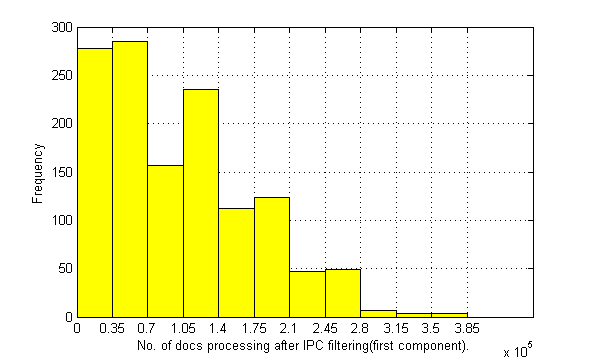
\includegraphics[width=0.70\textwidth,height=68mm]{figs/firstTwoIpcFilter-histo.png}
%   \caption{The distribution of the number of patents should be ranked for each query over all test queries (1303).
%In average, the matching process for each query is done over `$ 99754 $' documents instead of the whole collection (2.6 million documents) which reduce the computational time dramatically.}   
%   \label{fig:firstTwoIpcFilter-histo} 
%\end{figure}
%%%%%%%%%%%%%%%%%%%%%%%%%%%%%%%%%%%%%%%%%%%%%%%%%%%%%%%%%%%%%%%%%%%%%%%%%%%%%%%%%
%\FloatBarrier 
%\vspace{-5em}
%\noindent
%\subsubsection{Applying First two IPC code components for filtering}
%\label{subsec: Firsttwocomponents}
\paragraph{Filter Type III: First Component of IPC Code}
%\textbf{(C) Filter: First component of the IPC code}
\ \\
We can even make the filter more general by choosing only the first component, namely, section (e.g., C), corresponding to very general technical fields. 
%%%%%%%%%%%%%%%%%%%%%%%%%%%%%%%%%%%%%%%%%%%%%%%%%%%%%%%%%%%%%%
\begin{figure}[t!]
\begin{centering}
\subfigure[The portion of patents in the collection which are matched with the query IPC code. Filter: The first two components \label{fig:ipc1stElements_a}]{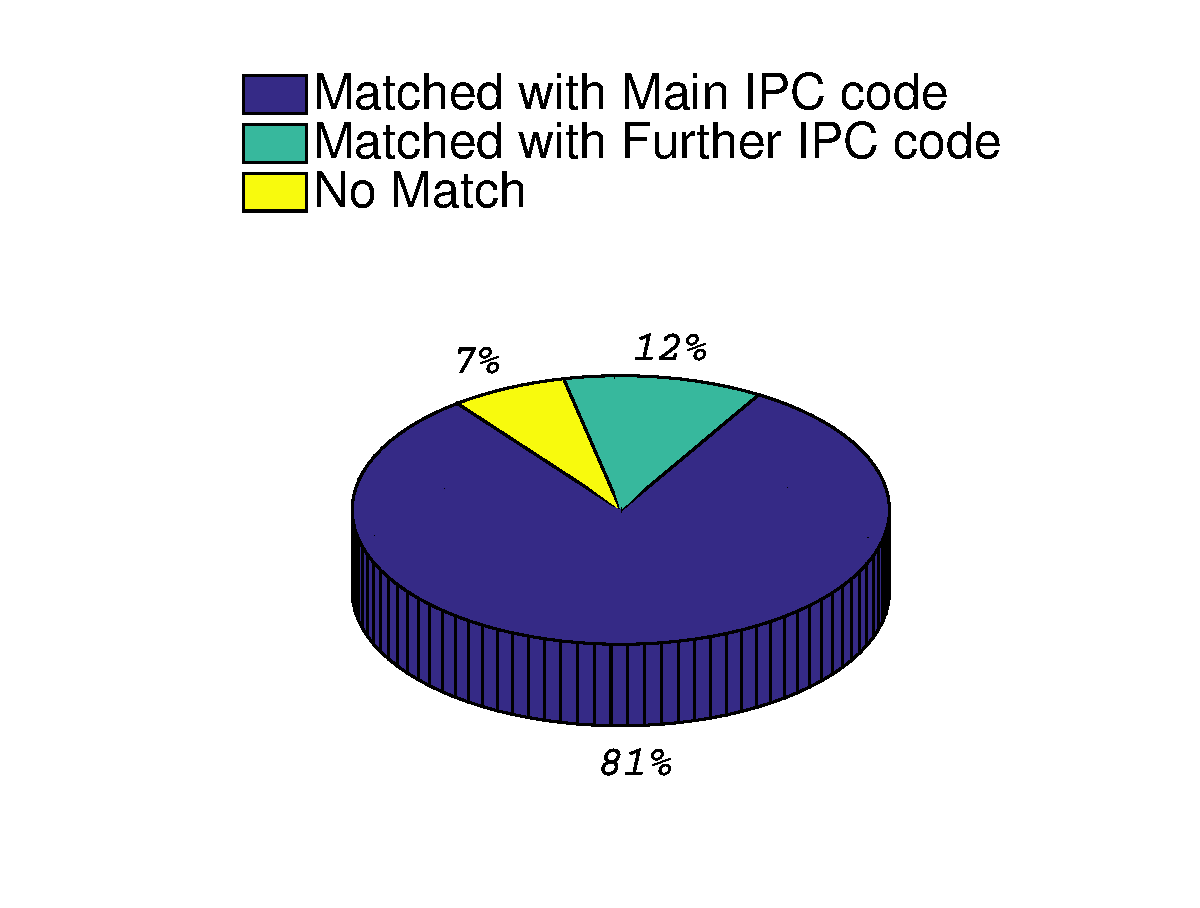
\includegraphics[width=7.5cm, height=6cm]{figs/filter3_pie}} 
\\[1ex]%
\subfigure[The distribution of the number of patents should be processed for each query after applying the IPC filter.
In average, the matching process for each query is done over $ 415,828 $ documents instead of the whole collection (2.6 million documents). This number is much higher than using more restricted filters, so it is not computationally~efficient.\label{fig:ipc1stElements_b}]{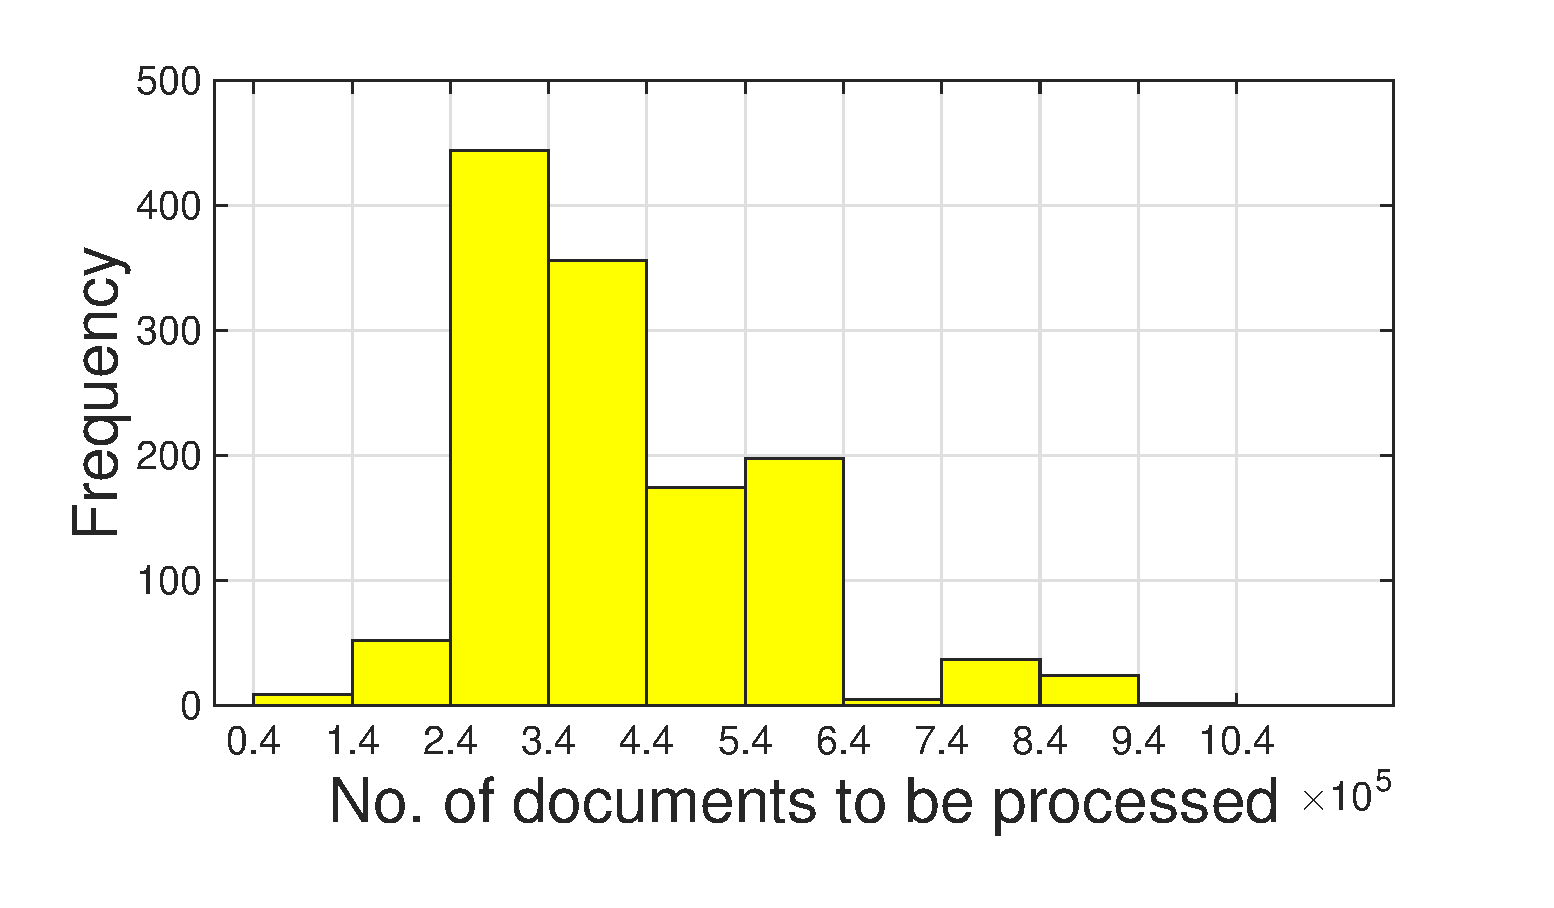
\includegraphics[width=9.5cm , height=6cm]{figs/filter3}} 

\par\end{centering} 
\protect\caption{Applying the first IPC code component for filtering (Section)}
\label{fig:ipc1stElements}
\end{figure}
%%%%%%%%%%%%%%%%%%%%%%%%%%%%%%%%%%%%%%%%%%%%%%%%%%%%%%%%%%%%%%
%%%%%%%%%%%%%%%%%%%%%%%%%%%%%%%%%%%%%%%%%%%%%%%%%%%%%%%%%%%%%%%%%%%%%%%%%%%%%%%%%
%\begin{figure}[t!]
%   \centering
%   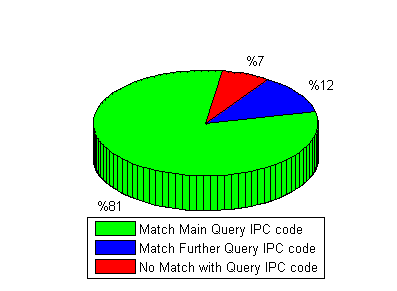
\includegraphics[width=0.50\textwidth,height=55mm]{figs/ipc1stElement.png}
%   \caption{Filter: Only the first component (Section).}   
%   \label{fig:ipc1stElements} 
%\end{figure}
%%%%%%%%%%%%%%%%%%%%%%%%%%%%%%%%%%%%%%%%%%%%%%%%%%%%%%%%%%%%%%%%%%%%%%%%%%%%%%%%%
Figure~\ref{fig:ipc1stElements_a} shows that about 7\% of relevant patents do not share the most general component of the query IPC Code. 
Figure~\ref{fig:ipc1stElements_b} shows the distribution of the number of patents should be ranked for each query after applying the IPC filter.
%: ``\textit{only the first component of the IPC code}". 
The results show that the matching process for each query is done over $ 415,828 $ documents, on average, instead of the whole collection (2.6 million documents). This number is much higher than the number for previous filters, which shows that using only the first component of the IPC code is not computationally efficient because it does not reduce the computational time as well as it still causes 7\% of the errors. 
%The min number of documents considered during matching process is `$ min=41721 $', and the maximum is `$ max=1058447 $'. 
%\vspace{-2em}
%%%%%%%%%%%%%%%%%%%%%%%%%%%%%%%%%%%%%%%%%%%%%%%%%%%%%%%%%%%%%%%%%%%%%%%%%%%%%%%%%
%\begin{figure}[t!]
%   \centering
%   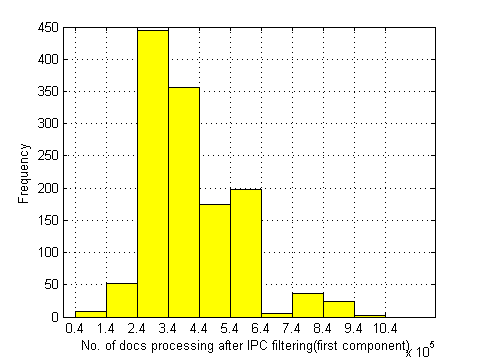
\includegraphics[width=0.60\textwidth,height=60mm]{figs/firstIpcFilter-histo.png}
%   \caption{The distribution of the number of patents should be ranked for a query over all test queries (1303), after applying the IPC filter: ``\textit{only the first component of the IPC code}".
%In average, the matching process for each query is done over `$ 415828 $' documents instead of the whole collection (2.6 million documents). This number is much higher than using more restricted filters and will not be efficient computationally. 
%%The min number of documents considered during matching process is `$ min=41721 $', and the maximum is `$ max=1058447 $'
%}   
%   \label{fig:firstIpcFilter-histo} 
%\end{figure}
%%%%%%%%%%%%%%%%%%%%%%%%%%%%%%%%%%%%%%%%%%%%%%%%%%%%%%%%%%%%%%%%%%%%%%%%%%%%%%%%%

To recap our experiments related to the IPC code filtering, we showed that, in trade off between the errors related to applying IPC code filter and computationally efficient matching process, we got the best results when we applied the first three IPC code (section, class, and subclass) of the reference query as a filter. The filter reduced the number of documents to be ranked from the whole collection to $ 36,254 $ documents on average, so using the IPC filter saved a considerable amount of computational time.
%%%%%%%%%%%%%%%%%%%%%%%%%%%%%%%%%%%%%%%%%%%%%%%%%%%%%%%%%%%%%%%%
%%%%%%%%%%%%%%%%%%%%%%%%%% Section 4 %%%%%%%%%%%%%%%%%%%%%%%%%%%
%%%%%%%%%%%%%%%%%%%%%%%%%%%%%%%%%%%%%%%%%%%%%%%%%%%%%%%%%%%%%%%%
%\section{New Evaluation: Excluding Identified Errors}
{
%\scriptsize
%\sffamily
\ttfamily\small
 \begin{tabular}{lcc}
 \hline\noalign{\smallskip} 
  & \multicolumn{1}{p{3cm}}{\centering Patent Query \\Not-Filtered} &\multicolumn{1}{p{3cm}}{\centering Patent Query \\Filtered} \\ 
 \noalign{\smallskip} 
\hline 
\noalign{\smallskip} 
\vtop{\hbox{\strut PRES}\hbox{\strut MAP}\hbox{\strut A. Recall}} 
& \vtop{\hbox{\strut 0.3910}\hbox{\strut 0.1214}\hbox{\strut 0.4008}}
& \vtop{\hbox{\strut 0.5355}\hbox{\strut 0.1618}\hbox{\strut 0.5491}} \\

\hline 
 \end{tabular} 
 
}
%%% Local Variables: 
%%% mode: latex
%%% TeX-master: t
%%% End: 
%%%%%%%%%%%%%%%%%%%%%%%%%%%%%%%%%%%%%%%%%%%%%%%%%%%%%%%%%%%%%%%%
%%%%%%%%%%%%%%%%%%%%%%%%%% Section 4 %%%%%%%%%%%%%%%%%%%%%%%%%%%
%%%%%%%%%%%%%%%%%%%%%%%%%%%%%%%%%%%%%%%%%%%%%%%%%%%%%%%%%%%%%%%%
%\section{Summary}
%\label{sce: summary3}
%We developed a baseline IR system for patent prior art search on the top of
the Lucene search engine\footnote{\texttt{http://lucene.apache.org/}}, which processes queries using both BM25~\cite{Robertson1993} and LM (Dirichlet
smoothing, and Jelinek-Mercer smoothing)~\cite{zhai2004study} scoring functions. %We consider 
%using BM25F~\cite{robertson2004simple} but had no opportunity to learn appropriate field weights.
We used Lucene to index the English subset of CLEF-IP 2010 dataset\footnote{\texttt{http://www.ifs.tuwien.ac.at/\textasciitilde{}clef-ip/}} 
(Section~\ref{sec:DataCollection}) that contains 2.6 million patent documents and 1303 topics (queries) for the English test set.
We used the default Lucene settings using the Porter stemming algorithm \cite{Porter1980} and English stop-word removal. 
We also removed patent-specific stop-words as described in \cite{magdy2012toward}.
In
our implementation, each section of a patent (title, abstract, claims,
and description) is indexed in a separate field. However, when a query 
is processed, all indexed fields are targeted with an equal weight, since this generally
offers best retrieval performance. We also used the International
Patent Classification (IPC) codes assigned to the topics to filter
the search results by constraining them to have common IPC codes with
the patent topic as suggested in previous works~\cite{lopez2010patatras}.
Although this IPC code filter may prevent retrieval of relevant patents, we
have chosen to keep it for the following reasons: (i) more than 80\%
of the patent queries share an IPC code with their associated relevant
patents, and (ii) it makes the retrieval process much faster. The accuracy of the results is evaluated using two popular metrics --- Mean Average Precision (MAP) and Average Recall --- on the top-100 results for each query, assuming that patent examiners are willing to assess the top 100 patents \cite{joho2010survey}. 
We achieved the best performance while querying with the Description
section as in previous work \cite{xue2009transforming} and using
either the LM or the BM25 scoring functions. We call this initial
query the \textit{Patent Query} and use it as our main baseline.

In addition, we compare our results to \textit{PATATRAS}, a highly engineered system developed by Lopez and Romary~\cite{lopez2010experiments}, which achieved the best performance in the CLEF-IP 2010 competition. This system uses multiple retrieval models (especially Kullback-Leibler divergence~\cite{Baeza-Yates2011} and Okapi BM25) and exploits patent metadata and citation structures.  While our evaluation excludes 22 of the 1303 topics for which no relevant English documents were available, the difference in MAP score between our evaluation and the full 1303 topic evaluation of PATATRAS is negligible. We exclude 22 queries because the focus of our research has been on term analysis and errors related to term matching process of ranking functions. So, we eliminated data curation errors and IPC filter errors--- as they will be described in Section~\ref{sec:DataCurationErrors} and Section~\ref{sec:ClassificationCodeMismatch}--- to increase the accuracy of our data analysis results. 
%did not include errors related to non-English patents in our evaluation and we mainly focus on errors related to term matching for English patents.  
%However, the MAP we provide is not directly comparable since we excluded 22 topics from our evaluation because their relevant patents were not in English or had no IPC code matched with the topic. We pruned these topics out because we were only interested in analysing errors related to term matching. Removing 22 topics caused only 0.04 improvement in our baseline system, which is negligible. Hence, we use Top CLEF-IP 2010 results for a rough comprasion."}
% 

% TODO: Don't exclude 22 topics!





%\chapter{Term Analysis}
\chapter{Optimal Query Term Selection}
\label{cha:analysis}
In this chapter, we will investigate the problem from term analysis perspective for both patent query and relevant documents because we are interested 
in finding what is wrong in term matching process between the patent query and relevant patents. 
We start with experiments that show sufficient term overlap between the patent query and relevant documents, 
then we introduce an oracular relevance feedback scoring criteria to discriminate useful terms from noisy terms. 
We formulate two oracular query, based on this score, that give us an upper-bound performance. In addition, our experiments demonstrate the sufficiency of terms in the patent query to achieve a high performance. 
We try four simple query reduction approaches and we discuss the reasons that they are not efficient.  
Finally, we show that we can get improved using a simple, minimal feedback interactive approach.
%%%%%%%%%%%%%%%%%%%%%%%%%%%%%%%%%%%%%%%%%%%%%%%%%%%%%%%%%%%%%%
%%%%%%%%%%%%%%%%%%%%%%%% SECTION 1 %%%%%%%%%%%%%%%%%%%%%%%%%%
%%%%%%%%%%%%%%%%%%%%%%%%%%%%%%%%%%%%%%%%%%%%%%%%%%%%%%%%%%%%%%

\section{Term Mismatch}
\label{sec:termmismatch}
%\input{TermAnalysis/termmismatch}
Standard retrieval models rank documents based on term matching between the query and documents.  
A significant term mismatch between the patent query and relevant patents has been mentioned the
main cause for low effective patent prior art search in previous works~\citep{roda2010clef}~\citep{magdy2012toward}. 
We examine term overlap between a patent query and three important subsets of documents for each query: (i) retrieved relevant patents (TPs); (ii) retrieved irrelevant patents (FPs); and (iii) not-retrieved relevant patents (FNs), respectively. We calculate the average term overlap per query as follows:
%%%%%%%%%%%%%%%%%%%%%%%%%%%%%%%%%%%%%%%%%%%%%%%%%%%%%%%%%%%%%%
\begin{equation} 
TO (Q) = \frac{1}{|D|}\sum_{d\in D}\frac{|terms_{Q\cap d}|}{|Q|},
\label{eq:fntermoverlap}
\end{equation}
%\vspace*{-1ex}
%\begin{displaymath}t\in \lbrace \mbox{terms in top-100 retrieved documents}\rbrace\end{displaymath}
%%%%%%%%%%%%%%%%%%%%%%%%%%%%%%%%%%%%%%%%%%%%%%%%%%%%%%%%%%%%%%
where $TO(Q)$ is the average term overlap per query, Q is a query in English subset of test queries (we calculate this score for TP, FP, and FN subsets, respectively), $D$ is a collection of TP patents, FP patents, or FN patents for each query, $|D|$ is the number of TP patents, FP patents, or FN patents for each query, $ |terms_{Q\cap d}| $ is the number of query terms appearing in each TP, FP, or FN patent, $ |Q| $ is the size of the query.

Figure~\ref{fig:overlap} compares the distribution of term overlap between the query and documents in three subsets (TP, FP, FN), over all queries in English test subset. We summarise the main conclusions for this experiment as follows:
\begin{enumerate}
\item For the majority of queries (around 94\% of queries), patent documents, which has the term overlap higher than $0.2$, are retrieved (e.g, TPs and FPs). 
\item We can also see sufficient term overlap with the query for FN patents, whereas, compared to TPs and FPs, more queries can be seen with the term overlap less than $ 0.2 $ (about 24\% of queries). 
\end{enumerate}
%%%%%%%%%%%%%%%%%%%%%%%%%%%%%%%%%%%%%%%%%%%%%%%%%%%%%%%%%%%%%%
\begin{figure}[t!]
%[htpb]
\begin{centering}
\subfigure[Query and TP patents.]{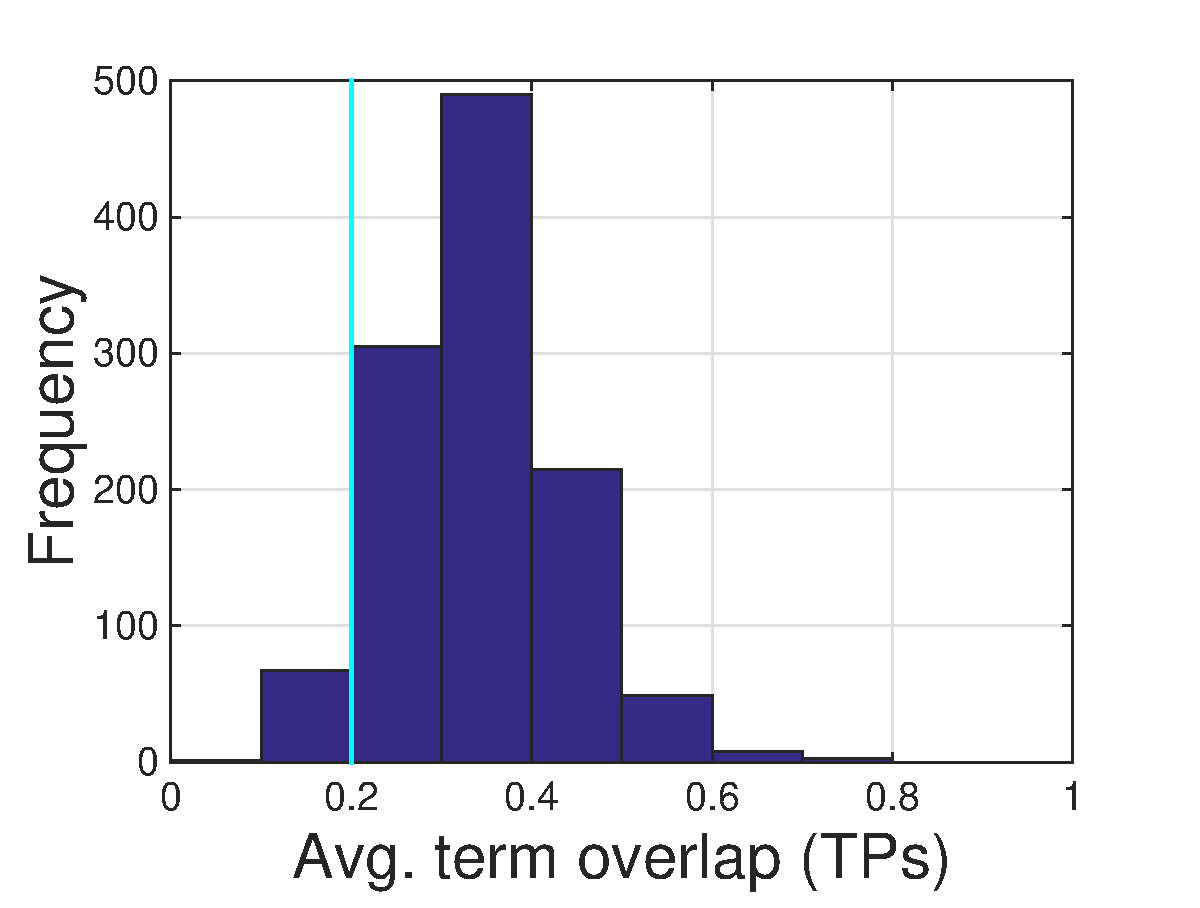
\includegraphics[width=5cm]{figs/to-tps.eps}}\subfigure[Query and FP patents.]{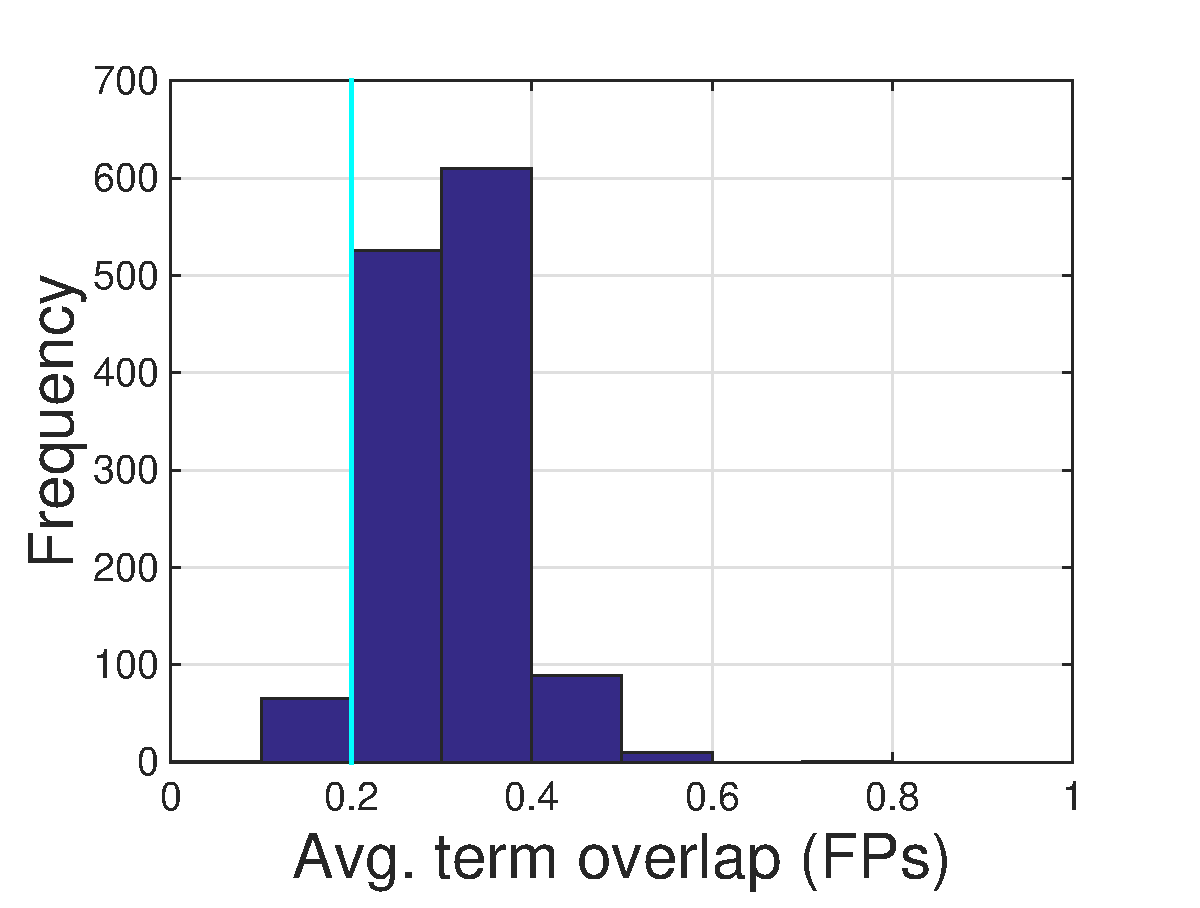
\includegraphics[width=5cm]{figs/to-fps.eps}}\subfigure[{Query and FN patents.}]{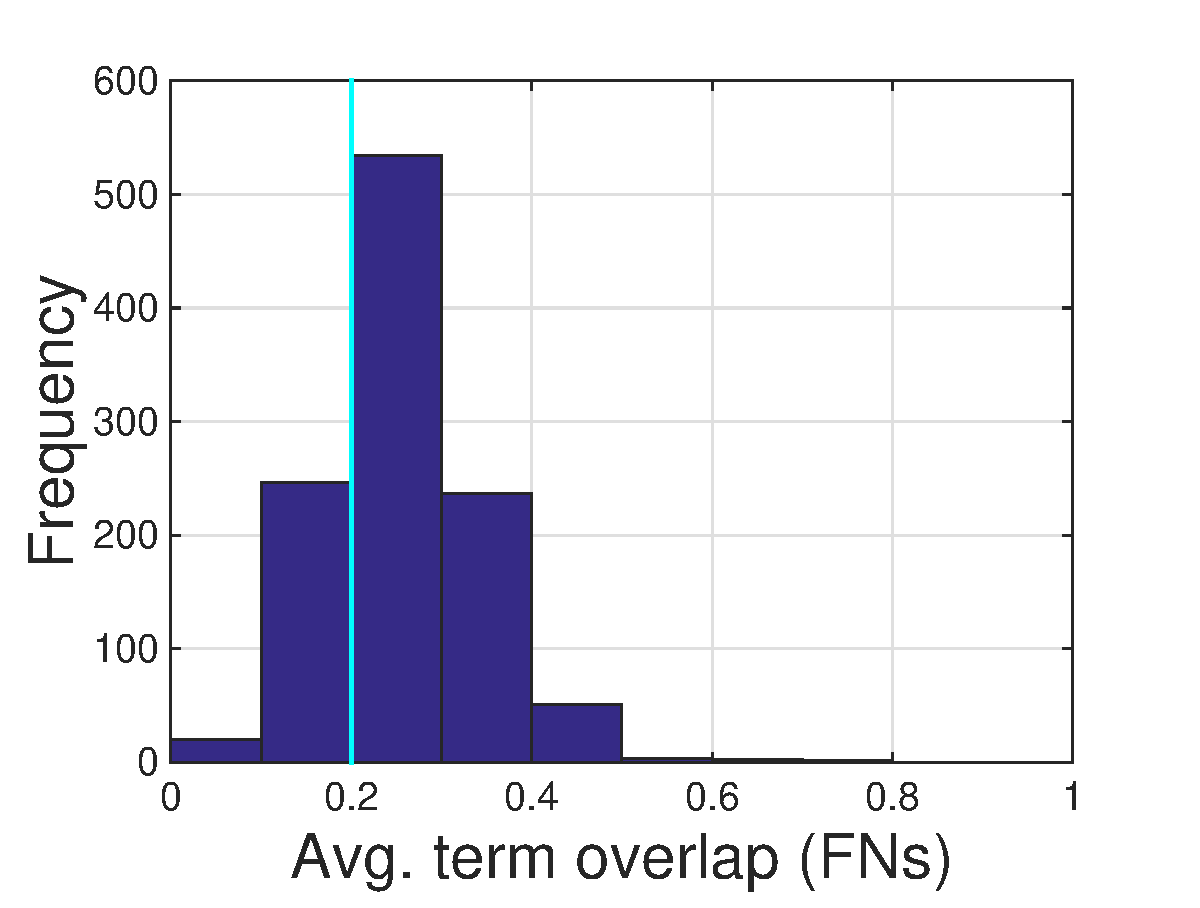
\includegraphics[width=5cm]{figs/to-fns.eps}}
\par\end{centering}

\protect\caption{The distribution of term overlap between the query and documents in three subsets (TP, FP, FN) over all queries in English test subset.}
\label{fig:overlap}
\end{figure}
%%%%%%%%%%%%%%%%%%%%%%%%%%%%%%%%%%%%%%%%%%%%%%%%%%%%%%%%%%%%%%
This experiment implicitly shows that a low or zero term match is not the main cause of low effectiveness in patent prior art search. In the next session, we explain a method to discriminate between the terms, which help the retrieval of relevant documents from those, which are not useful. 
%%%%%%%%%%%%%%%%%%%%%%%%%%%%%%%%%%%%%%%%%%%%%%%%%%%%%%%%%%%%%%
%%%%%%%%%%%%%%%%%%%%%%%%% SECTION 2 %%%%%%%%%%%%%%%%%%%%%%%%%%
%%%%%%%%%%%%%%%%%%%%%%%%%%%%%%%%%%%%%%%%%%%%%%%%%%%%%%%%%%%%%%
\section{Oracular Relevance Feedback System}
\label{sec:oraculrquery}
A query is optimal if it ranks all relevant documents before
those that are not relevant, it would lead to a ranking with an average precision of $1.0$. A query
is most likely to achieve a ranking that is as close to optimal as possible if it contains all terms that
appear in all relevant documents, but explicitly discounts all terms that occur in irrelevant documents~\citep{manning2008introduction}.

Inspired by the optimal query idea, we develop an oracular relevance feedback system, which
extracts terms from the judged relevant documents to derive an upper bound on performance of
standard Okapi BM25 and LM retrieval
algorithms for patent prior art search.
We, first, use the oracular relevance feedback to score query terms. 
Then, we run some experiments related to the existence of the useful terms inside the patent query.   
Finally, we analyse the system performance for two oracular query formulated by useful terms. 
%\subsection{Oracular Term Selection}
\subsection{Term Scoring}
\label{OracularTermSelection}
After an initial run of the patent query, we build a vocabulary set out of all terms appearing in top-100 retrieved documents; then we use judged relevant documents to score each term. 
We calculate an oracular relevance feedback score ($RF(t,Q)$) for each term $t$ in the top-100
retrieved documents given the query $Q$ as follows:
%%%%%%%%%%%%%%%%%%%%%%%%%%%%%%%%%%%%%%%%%%%%%%%%%%%%%%%%%%%%%%
\begin{equation}
RF(t,Q)=Rel(t)-Irr(t), 
 \label{eq:rfscore}
\end{equation}
\begin{displaymath}t\in \lbrace \mbox{terms in top-100 retrieved documents}\rbrace,\end{displaymath}
%%%%%%%%%%%%%%%%%%%%%%%%%%%%%%%%%%%%%%%%%%%%%%%%%%%%%%%%%%%%%%
where $ \mathit{Rel(t)} $ is the average term frequency in retrieved relevant patents, and $ \mathit{Irr(t)} $ is the average term frequency in retrieved irrelevant patents. According to the Equation \ref{eq:rfscore}, words appearing more frequently in relevant documents achieve higher RF score. We might assume that words, with a positive score, are \textit{useful terms} because they are more frequent in relevant patents while words, with a negative score, are \textit{noisy terms} because they appear more frequently in irrelevant patents. However in the following experiments, we empirically seek a threshold $\tau$ to pick useful terms. 

We yield the oracular relevance feedback score to: (i) find a pattern for the system performance versus useful terms; (ii) show the term overlap with useful terms and noisy terms for TP, FN patents; (iii)  examine the existence of useful terms in different sections of the patent query.
\subsection{Performance versus Useful Terms}
\label{PerformanceUsefulTerms}
%\paragraph{Performance versus Useful Terms}
%\ \\
We, intuitively, expect that queries, which contain more useful terms achieve higher performance. Hence in this experiment,
we investigate if more useful terms in the reference patent query leads to a higher performance. In other words, we seek for a pattern between the performance and the existence of the useful terms in initial patent query. 

We define four different criteria to select useful terms as follows:
\begin{enumerate}
\item terms with positive RF scores ($ RF(t, Q)>0) $);
\item terms with the score higher than the positive median score\\ ($ RF(t, Q)>RF(t_{+median}, Q) $);
\item terms with the score higher than a constant: 1, 5, and 10 ($ RF(t, Q)>1, 5, 10) $);
\item top-100 high-scored terms.
\end{enumerate}
For each query, we calculate the fraction of useful terms to all query terms. 
Figure~\ref{fig:overlap-r} shows the scatter plot of the recall versus this fraction. 
As it can be seen, unlike our first assumption, we do not see any correlation between the recall and the presence of useful terms in the query and the pattern for the recall is very noisy and irregular. 
We repeat the experiment for the average precision (AP). Figure~\ref{fig:overlap-p} shows the scatter plot of the AP versus the existence of useful terms in the query. Although it is slightly better than the recall and we can see a very weak correlation between AP and useful terms inside the query for top-scored words (e.g., $RF(t, Q)>10$), it does not demonstrate our first conjecture. 
This experiment also implicitly indicates that term mismatch between the patent query and relevant documents is 
not the main reason for the low effectiveness of the patent prior art search. 
%%%%%%%%%%%%%%%%%%%%%%%%%%%%%%%%%%%%%%%%%%%%%%%%%%%%%%%%%%%%%%
\begin{figure}[t!]
\begin{centering}
\subfigure[Useful terms: $ \{t|RF(t, Q)>0\} $]{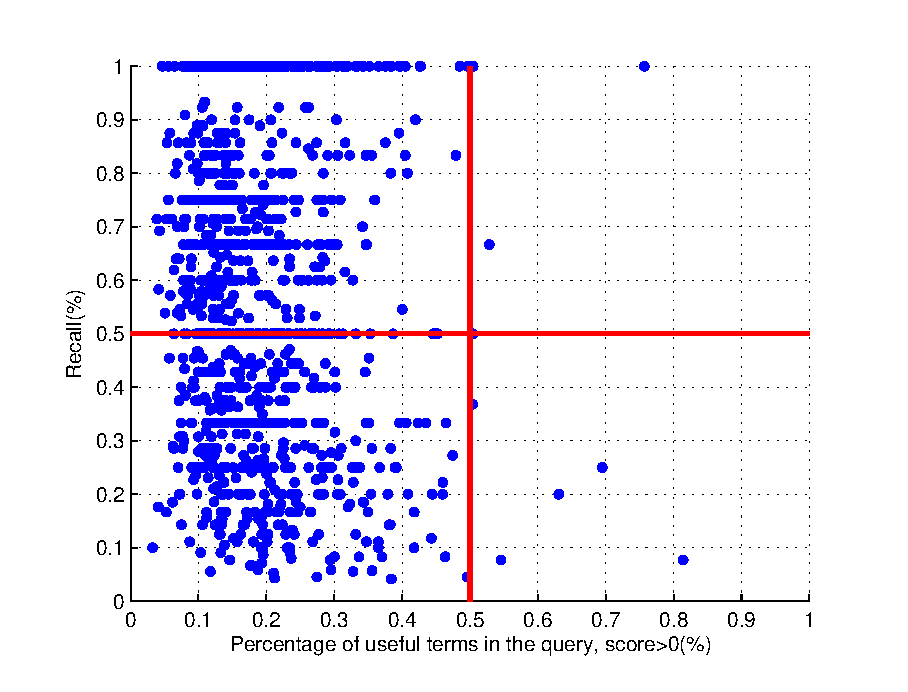
\includegraphics[width=6cm]{figs/greaterthan0-r.eps}} \hspace*{1.5cm} \subfigure[Useful terms: $ \{t|RF(t, Q)>RF(t_{+median})\} $]{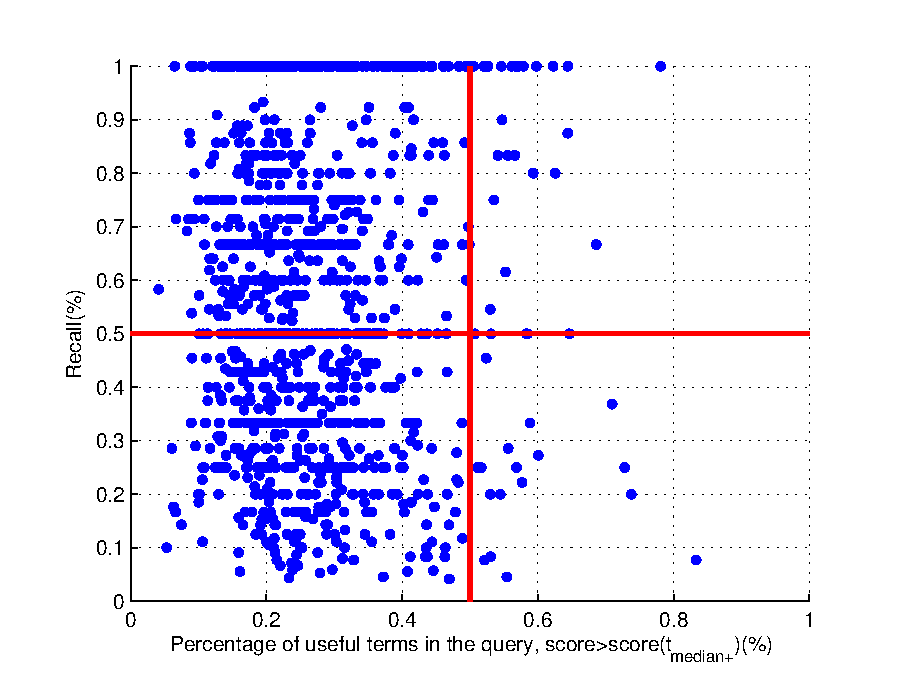
\includegraphics[width=6cm]{figs/greaterthanmedian-r.eps}}\\ \subfigure[{Useful terms: $ \{t|RF(t, Q)>1 \}$}]{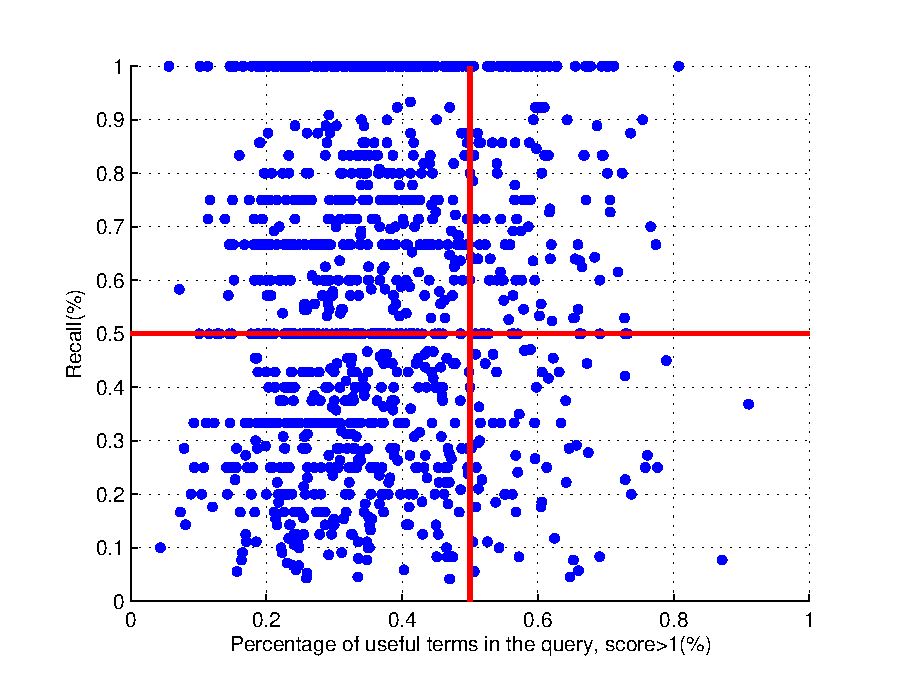
\includegraphics[width=6cm]{figs/greaterthan1-r.eps}} \hspace*{1.5cm} \subfigure[{Useful terms: top 100 high-scored terms}]{\includegraphics[width=6cm]{figs/top100-r.eps}}\\ \subfigure[{Useful terms: $ \{t|RF(t,Q)>5 \}$}]{\includegraphics[width=6cm]{figs/greaterthan5-r.eps}} \hspace*{1.5cm} \subfigure[{Useful terms: $ \{t|RF(t, Q)>10\} $}]{\includegraphics[width=6cm]{figs/greaterthan10-r.eps}}
\par\end{centering}

\protect\caption{Scatter plot of recall versus the existence of useful terms in query.}
\label{fig:overlap-r}
\end{figure}
%%%%%%%%%%%%%%%%%%%%%%%%%%%%%%%%%%%%%%%%%%%%%%%%%%%%%%%%%%%%%%
%%%%%%%%%%%%%%%%%%%%%%%%%%%%%%%%%%%%%%%%%%%%%%%%%%%%%%%%%%%%%%
\begin{figure}[t!]
\begin{centering}
\subfigure[Useful terms: $ \{t|RF(t, Q)>0\} $]{\includegraphics[width=6cm]{figs/greaterthan0-p}} \hspace*{1.5cm} \subfigure[Useful terms: $ \{t|RF(t, Q)>RF(t_{+median}, Q)\} $]{\includegraphics[width=6cm]{figs/greaterthammedian-p.eps}} \\%[-2ex]% 
\subfigure[{Useful terms: $ \{t|RF(t, Q)>1 \}$}]{\includegraphics[width=6cm]{figs/greaterthan1-p.eps}} \hspace*{1.5cm} \subfigure[{Useful terms: top 100 high-scored terms}]{\includegraphics[width=6cm]{figs/top100-p.eps}}\\ %[-2ex]%
\subfigure[{Useful terms: $ \{t|RF(t,Q)>5 \}$}]{\includegraphics[width=6cm]{figs/greaterthan5-p.eps}} \hspace*{1.5cm} \subfigure[{Useful terms: $ \{t|RF(t, Q)>10\} $}]{\includegraphics[width=6cm]{figs/greaterthan10-p.eps}}
\par\end{centering}

\protect\caption{Scatter plot of average precision (AP) versus the existence of useful terms in query.}
\label{fig:overlap-p}
\end{figure}
%%%%%%%%%%%%%%%%%%%%%%%%%%%%%%%%%%%%%%%%%%%%%%%%%%%%%%%%%%%%%%
\subsection{Term Overlap with Useful Terms and Noisy Terms}
%\paragraph{Term Overlap with Useful Terms and Noisy Terms}
%\ \\
In the second experiment, we check the term overlap with useful terms and noisy terms for TP and FP patents. Figure \ref{fig:usefulnoisy} shows that relevant patents have a higher term overlap with the useful terms while irrelevant patents have a higher term overlap with the noisy terms. This experiment shows that noisy terms cause the system to retrieve irrelevant patents at top of the list. 
%%%%%%%%%%%%%%%%%%%%%%%%%%%%%%%%%%%%%%%%%%%%%%%%%%%%%%%%%%%%%%
\begin{figure}[t!]
%[htpb]
\begin{centering}
\subfigure[TPs]{\includegraphics[width=6cm]{figs/stackedTPs.eps}} \hspace*{1.5cm} \subfigure[FPs]{\includegraphics[width=6cm]{figs/stackedFPs.eps}} 
\par\end{centering} 

\protect\caption{The distribution of the term overlap between the query and useful terms/noisy terms in TPs and FPs. Relevant patents have higher term overlap with useful terms while irrelevant patents have higher term overlap with noisy terms.}
\label{fig:usefulnoisy}
\end{figure}
%%%%%%%%%%%%%%%%%%%%%%%%%%%%%%%%%%%%%%%%%%%%%%%%%%%%%%%%%%%%%%
%We hypothesized that a query, formulated by only the \textit{ useful terms}, is the best possible query we can make since they are all frequent in relevant patents but rare in irrelevant ones. 
\subsection{Useful Terms in Different Sections of Patents}
%\paragraph{Useful Terms in Different Sections of Patents}
%\ \\
%%%%%%%%%%%%%%%%%%%%%%%%%%%%%%%%%%%%%%%%%%%%%%%%%%%%%%%%%%%%%%
\begin{table*}[t!]
  \begin{center}
   \caption{Average number of useful terms in the different sections of patent query}
  \input table/usefultermsinsections.tex   
  \label{tab:usefultermsinsections}
  \end{center}  
\end{table*}
%\FloatBarrier
%%%%%%%%%%%%%%%%%%%%%%%%%%%%%%%%%%%%%%%%%%%%%%%%%%%%%%%%%%%%%%
%%%%%%%%%%%%%%%%%%%%%%%%%%%%%%%%%%%%%%%%%%%%%%%%%%%%%%%%%%%%%%
\begin{table*}[t!]
  \begin{center}
   \caption{Average percentage of useful terms in the different sections of patent query}
  \input table/usefultermsinsections-p.tex   
  \label{tab:usefultermsinsections-p}
  \end{center}  
\end{table*}
%%%%%%%%%%%%%%%%%%%%%%%%%%%%%%%%%%%%%%%%%%%%%%%%%%%%%%%%%%%%%%
Patents are structured documents containing title, abstract, description, and claims (Section~\ref{StructureofPatents}). In this experiment, we investigate the existence of useful terms in different sections of patents. 
Table \ref{tab:usefultermsinsections} shows the average number of useful terms in different sections of a patent query.  
As it can be seen, description has the highest number of useful terms in both cases where RF score threshold $ \tau $ is $0$ and $1$. When $ \tau = 0 $, the average number of the useful terms in description is quite twice of when $ \tau = 1 $. Compared to other sections, description contains more useful terms, which proves why we achieved higher performance querying with description (Section~\ref{sec:settings}).
Table \ref{tab:usefultermsinsections-p} shows the average percentage of useful terms in different sections of a patent query. It shows that, overall, useful terms constitute less than 50\% of the whole words in each section of patent queries. For example, we can see that only 27\% of the whole patent query in average are useful terms and the rest are irrelevant terms. 
%\subsubsection{Useful Terms in Different Sections}
\subsection{Oracular Query Formulation}
\label{sec:OracularQueryFormulation}
As we illustrated in Section~\ref{PerformanceUsefulTerms}, we could not find an informative pattern for the performance and the existence of the useful terms in patent query.
In this section, we examine the system effectiveness for queries formulated by terms selected by oracular relevance feedback system.
We formulate two different oracular queries.

The first query is formulated by selecting terms in the top-100 retrieved documents using oracular relevance feedback score and we call it oracular query:
%%%%%%%%%%%%%%%%%%%%%%%%%%%%%%%%%%%%%%%%%%%%%%%%%%%%%%%%%%%%%%
\begin{equation}
Oracular \; Query = \{t \in top-100|RF(t, Q)>\tau\}.   
 \label{eq:score}
\end{equation}
%%%%%%%%%%%%%%%%%%%%%%%%%%%%%%%%%%%%%%%%%%%%%%%%%%%%%%%%%%%%%% 
%%%%%%%%%%%%%%%%%%%%%%%%%%%%%%%%%%%%%%%%%%%%%%%%%%%%%%%%%%%%%%
\begin{figure}[t!]
\begin{centering}
\subfigure[oracular query performance versus the threshold $\tau$.\label{fig:oracular-a}]{\includegraphics[width=6cm]{figs/oracularq.eps}} \hspace*{.5cm} \subfigure[oracular query performance versus the query size.\label{fig:oracular-b}]{\includegraphics[width=6cm]{figs/oracularq-size.eps}} 
\par\end{centering} 
\protect\caption{oracular query performance versus various values of the threshold $\tau$ and query size}
\label{fig:oracular}
\end{figure}
%%%%%%%%%%%%%%%%%%%%%%%%%%%%%%%%%%%%%%%%%%%%%%%%%%%%%%%%%%%%%%
We empirically seek to evaluate the threshold $\tau$ on $RF(t,Q)$ and query size yielding the best oracular query.
Table~\ref{tab:optquery} and Figure~\ref{fig:oracular-a} show that the oracular query far outperform the baseline query (reference patent query), and it approximately performs twice as well on the PATATRAS system, the best competitor in CLEF-IP 2010 system. In Table~\ref{tab:optquery}, we also compare the influence of weighed and unweighed terms for both baseline query and oracular query. It can be seen that weighing terms in patent query with their frequency helps the performance while weighing terms in oracular query with $RF(t, Q)$ harms the performance. 
Figure \ref{fig:oracular-a} shows how the performance changes by the values of $\tau$. We remark two important facts as follows: 
\begin{enumerate}
\item Including slightly noisy terms (i.e., $\tau$ just slightly less than 0) leads in an unexpected steep drop-off in performance.  
\item We achieve the highest MAP for the oracular query formulated by selecting the terms with $RF(t, Q)>0$.
\end{enumerate}
Figure~\ref{fig:oracular-b} shows that the performance increases notably when we include terms up to 200 while formulating a query, but it remains quit unchanged when we include more than 200 terms. 
%%%%%%%%%%%%%%%%%%%%%%%%%%%%%%%%%%%%%%%%%%%%%%%%%%%%%%%%%%%%%%
\begin{table}[t!]
  \begin{center}
  \scriptsize
   \caption{Performance for the patent query (PQ/baseline), two variants of the oracular query (OracularQ, OracularPQ), and Top CLEF-IP 2010 Competitor (PATATRAS).}
   \vspace*{1ex}
  \input table/optquery.tex   
  \label{tab:optquery}
  \end{center}  
\end{table}
%%%%%%%%%%%%%%%%%%%%%%%%%%%%%%%%%%%%%%%%%%%%%%%%%%%%%%%%%%%%%%
%Next, inspired by Maxwell and Croft's work~\citep{maxwell2013compact} that emphasise on the importance of query words, 
We seek to establish that the terms within a reference patent query are sufficient for a strong performance, so, we formulate the second query by selecting oracular terms that also occur in the reference patent query. We call it oracular patent query:
%%%%%%%%%%%%%%%%%%%%%%%%%%%%%%%%%%%%%%%%%%%%%%%%%%%%%%%%%%%%%%
\begin{equation}
 Oracular \; Patent \; Query = \{t\in Q|RF(t, Q)>\tau\}.   
 \label{eq:score}
\end{equation}
%%%%%%%%%%%%%%%%%%%%%%%%%%%%%%%%%%%%%%%%%%%%%%%%%%%%%%%%%%%%%%
%%%%%%%%%%%%%%%%%%%%%%%%%%%%%%%%%%%%%%%%%%%%%%%%%%%%%%%%%%%%%%
\begin{figure}[t!]
\begin{centering}
\includegraphics[width=9cm]{figs/l1}
\par\end{centering}

\begin{centering}
\subfigure[Mean Average Precision $\tau$.\label{fig:oracularpq-a}]{\includegraphics[width=6cm]{figs/fig1_map.eps}} 
\hspace*{1.5cm} \subfigure[Average Recall\label{fig:oracularpq-b}]{\includegraphics[width=6cm]{figs/fig1_recall.eps}} 
\par\end{centering} 

\protect\caption{Comparing the performance of oracular query and oracular patent query for various values of the threshold $\tau$}
\label{fig:oracularpq}
\end{figure}
%\begin{figure}[t!]
%   \centering
%   \includegraphics[width=0.50\textwidth,height=55mm]{figs/oracularpq.eps}
%   \caption{oracular patent query performance versus the threshold $\tau$.}   
%   \label{fig:oracularpq} 
%\end{figure}
%%%%%%%%%%%%%%%%%%%%%%%%%%%%%%%%%%%%%%%%%%%%%%%%%%%%%%%%%%%%%%
\paragraph{Analyse the results}
\ \\
As it has been shown in Table~\ref{tab:optquery} and Figure~\ref{fig:oracularpq}, the system performance for the oracular patent query is also considerably improved compared to the baseline and PATATRAS.
% though MAP is slightly less than Oracular Query. 
The results indicate that the patent query has sufficient terms for an improved performance. 
We compare MAP and recall for both oracular query and oracular patent query in Figure~\ref{fig:oracularpq}. 
On one hand, we notice that MAP for oracular patent query is slightly less than MAP for oracular query. We justify that it is due to some extra terms in top-100 vocabulary set that they are absent within the patent query. On the other hand, oracular patent query performance drops slower for negative values of $\tau$, which shows that oracular patent query contains less noisy terms than oracular query. 
This explains why query expansion techniques is not too effective for patent prior art search. We also conclude that the the existence of the noisy terms is the main cause of low effectiveness in prior art search.  

To recap, our experiments related to oracular relevance feedback system
suggest two important conclusions: 
\begin{enumerate}
\item Query reduction should suffice for effective prior art patent retrieval.
\item Very precise methods for eliminating poor query terms in the reduction process are required.
\end{enumerate}
%\subsection{Discriminative Words}
%\label{sec:discriminative}
%
%\subsection{RF Optimal Query Formulation}
%\label{sec:formulation}
%%%%%%%%%%%%%%%%%%%%%%%%%%%%%%%%%%%%%%%%%%%%%%%%%%%%%%%%%%%%%%
%%%%%%%%%%%%%%%%%%%%%%%%% SECTION 3 %%%%%%%%%%%%%%%%%%%%%%%%%%
%%%%%%%%%%%%%%%%%%%%%%%%%%%%%%%%%%%%%%%%%%%%%%%%%%%%%%%%%%%%%%
\section{Query Reduction: Approximating the Oracular Patent Query}
\label{sec: QR}
The gain achieved using the oracular patent query method motivates us to explore various methods to approximate the terms
selected by this query without ``peeking at the answers'' provided by
the actual relevance judgements.  We first attempt this via fully
automated methods and then proceed to evaluate semi-automated methods
based on interactive relevance feedback methods.
\subsection{Automated Reduction}
\label{AutomatedReduction}
For automated reduction we first examine three simple approaches, then we apply pseudo relevance feedback for query term selection.  
\subsubsection{Simple Query Reduction Approaches}
%%%%%%%%%%%%%%%%%%%%%%%%%%%%%%%%%%%%%%%%%%%%%%%%%%%%%%%%%%%%%%
\begin{figure}[t!]
\begin{centering}
\includegraphics[width=9cm]{figs/l3}
\par\end{centering}

\begin{centering}
\subfigure[Mean Average Precision.]{\includegraphics[width=6cm]{figs/fig3_map}} \hspace*{1.5cm} \subfigure[Average Recall.]{\includegraphics[width=6cm]{figs/fig3_recall}} 
\par\end{centering} 

\protect\caption{Comparing system performance for three different query reduction approaches and their changes with a threshold $\tau$.}
\label{fig:combinedapproach}
\end{figure}
%%%%%%%%%%%%%%%%%%%%%%%%%%%%%%%%%%%%%%%%%%%%%%%%%%%%%%%%%%%%%%
\label{SimpleApproaches}
We, first, apply three simple approaches to reduce the initial patent queries aiming at approximating the oracular patent query: (i) removing document frequent terms; (ii) removing less frequent terms in patent query; (iii) removing terms in IPC titles.
\paragraph{Removing Document Frequent Terms}
\ \\
In standard IR, removing terms appearing highly frequently across documents in the collection can improve retrieval effectiveness~\citep{manning2008introduction}. Inspired by this fact, we hypothesize that we will improve the performance by pruning out highly frequent words in top-100 retrieved documents after an initial run of patent query. To identify highly frequent terms, we calculate the average term frequency over top-100 documents for each word and we call it Document Frequent ($\mathit{DF}$) score, as follows:
%%%%%%%%%%%%%%%%%%%%%%%%%%%%%%%%%%%%%%%%%%%%%%%%%%%%%%%%%%%%%%
\begin{equation}
 DF(t, Q)=\frac{1}{100}\sum_{d_i\in  D} TF(t, d_i),    
 \label{eq:df}
\end{equation}
where $D=\{d\in \mbox{Top-100 retrieved documents}\}$, and $TF(t, d_i)$ is the term frequency of each term in document $d_i$.
%\begin{displaymath}   t\in \lbrace \mbox{terms in top-100 retrieved documents}\rbrace\end{displaymath}
%%%%%%%%%%%%%%%%%%%%%%%%%%%%%%%%%%%%%%%%%%%%%%%%%%%%%%%%%%%%%%

We remove words with $\mathit{DF}$ score higher than $\tau$ ($DF(t, Q)>\tau$) from patent query. Figure~\ref{fig:combinedapproach} illustrates how the performance change by different values of the threshold $\tau$ illustrates that removing document frequent words for different threshold $\tau$ hurts the performance (magenta line). As it can be seen, the performance converges with the baseline performance when $\tau$ goes higher (e.g., 500). This means that there is no term with such a high DF score, and we do not empirically remove any term from the patent query. Overall, removing document frequent terms from patent query does not consider an appropriate approach since it ruins the performance. 
\paragraph{Removing Less Frequent Terms in Patent Query}
\ \\
Frequent terms inside long and verbose queries are considered important~\citep{maxwell2013compact}. However, we hypothesise that we may improve the effectiveness by removing terms appearing less frequently in the patent query. Therefore, we remove terms with the frequency less than the threshold $\tau$ ($QTF(t)<=\tau$ ). The blue line in Figure~\ref{fig:combinedapproach} indicates that the performance gets slightly better than the baseline when we remove less frequent terms in patent query. As it can be seen the best MAP achieved when $\tau=5$. 
%In this approach the best value for the threshold is $\tau=5$ to get higher MAP.
\paragraph{Removing Terms in IPC Titles}
\ \\
The titles of classification indicate their intended content by using a single phrase or several related phrases linked together. We used words in IPC code titles for each patent query to reduce the query, based on the assumption that they are common to all patents belonging to the same category and may be considered as stop-words. As it can be seen in Figure~\ref{fig:combinedapproach} (red line), this approach slightly helps the performance.

We showed in above experiments that removing document frequent terms did not help the effectiveness and 
two other approaches had a trivial influence on improving the system effectiveness. 
In the following experiment, we use an anecdotal example of a sample patent query to analyse why these approaches did not help. 
Figure~\ref{fig:scatter_combined} shows a scatter plot of DF score and RF score for a sample query --- PAC-1612. Each blue point is a vocabulary in top-100 retrieved document vocabulary set. First, we remark a negative correlation between $\mathit{DF(t, Q)}$ and $\mathit{RF(t, Q)}$, however, it does not help because as it has been illustrated in Figure~\ref{fig:scatter_combined_b}, by removing document frequent terms ($DF(t, Q)>\tau$), we will remove many useful terms ($RF(t, Q)>0$). Red points in Figure~\ref{fig:scatter_combined_a} are all query terms and red points in Figure~\ref{fig:scatter_combined_b} are query terms with term frequency higher than 5 ($QTF(t)>5$) --- where we got the best performance. 
Comparing Figures~\ref{fig:scatter_combined_a} and ~\ref{fig:scatter_combined_b} show that we remove considerable amount of noisy terms by removing terms with $QTF(t)<5$. 
On the other hand, it can be seen that many useful terms are also removed. Remained terms are not purely useful terms since they are contaminated with the noisy terms. We conclude that we achieve a trivial improvement over the baseline because proposed reduction techniques cannot precisely filter the noisy terms out. 
%%%%%%%%%%%%%%%%%%%%%%%%%%%%%%%%%%%%%%%%%%%%%%%%%%%%%%%%%%%%%%%%%%%%%%%%%%%%%%%%%%%%%%%%%%%%%%%%%%%%%%%%%%% 
%%%%%%%%%%%%%%%%%%%%%%%%%%%%%%%%%%%%%%%%%%%%%%%%%%%%%%%%%%%%%%
\begin{figure}[t!]
\begin{centering}
\subfigure[Query terms ($t \in Query$) versus Document Frequent terms.\label{fig:scatter_combined_a}]{\includegraphics[width=9cm]{figs/qterm_rf_df.eps}} \hspace*{0.1cm}\\[1ex]% 
 %\subfigure[IPC Title words vs. Document Frequent terms.\label{fig:scatter_combined_b}]{\includegraphics[width=7cm]{figs/ipcdef-rf-df.eps}} 
\subfigure[Query terms ($t \in Query \; \bigwedge \; QTF(t)>5$) versus Document Frequent terms\label{fig:scatter_combined_b}]{\includegraphics[width=9cm]{figs/df-rf-tauline.eps}}

\par\end{centering}

\protect\caption{Anecdotal example for simple query reduction approaches. Blue points are all terms in a vocabulary set made of top-100 retrieved documents and red points are terms in the patent query.}
\label{fig:scatter_combined}
\end{figure}
%%%%%%%%%%%%%%%%%%%%%%%%%%%%%%%%%%%%%%%%%%%%%%%%%%%%%%%%%%%%%%
\subsubsection{Query Reduction Using Pseudo Relevance Feedback}
% TODO: Must be consistent in either pruning or removing terms --- results should ideally converge to the baseline at 0.
% TODO: Should do simplest comparisons first and not combine pruning approaches.  Even better: evaluate methods mentioned in related work.
% TODO: What is an IPC title?  I don't know that this is... was it discussed?
Pseudo Relevance Feedback ($\mathit{PRF}$) is an automated process without user interaction which assumes the top k ranked documents are relevant and the others are irrelevant~\citep{Baeza-Yates2011}. We use $\mathit{PRF}$ to select query terms~\cite{maxwell2013compact} the same as what we did for oracular relevance feedback system (Section~\ref{sec:oraculrquery}). We assume that top 5 retrieved documents are relevant and the rest are irrelevant, then we calculate $\mathit{PRF}$ score based on this assumption:  
%%%%%%%%%%%%%%%%%%%%%%%%%%%%%%%%%%%%%%%%%%%%%%%%%%%%%%%%%%%%%%
\begin{equation}
PRF(t,Q)=Rel(t)-Irr(t), 
 \label{eq:score}
\end{equation}
\vspace*{-2ex}
\begin{displaymath}t\in \lbrace \mbox{terms in top-100 retrieved documents}\rbrace\end{displaymath}.
%%%%%%%%%%%%%%%%%%%%%%%%%%%%%%%%%%%%%%%%%%%%%%%%%%%%%%%%%%%%%%  
In the next step, we select the terms in the patent query that have the $\mathit{PRF}$ score higher than the threshold $\tau$ ($PRF(t)>\tau$) to reformulate a reduced query. Figure~\ref{fig:prf} shows slight improvement over the baseline. Compared to the oracular term selection system, this approach did not also help to get any notable improvement over the baseline.
%%%%%%%%%%%%%%%%%%%%%%%%%%%%%%%%%%%%%%%%%%%%%%%%%%%%%%%%%%%%%%
\begin{figure}[t!]
   \centering
   \includegraphics[width=0.50\textwidth,height=55mm]{figs/prf.eps}
   \caption{Query reduction using PRF for various value of the threshold $\tau$.}   
   \label{fig:prf} 
\end{figure}
%%%%%%%%%%%%%%%%%%%%%%%%%%%%%%%%%%%%%%%%%%%%%%%%%%%%%%%%%%%%%%
%%%%%%%%%%%%%%%%%%%%%%%%%%%%%%%%%%%%%%%%%%%%%%%%%%%%%%%%%%%%%%
\begin{figure}[t!]
\begin{centering}
\subfigure[$\tau=0$\label{fig:rf_prf_a}]{\includegraphics[width=7cm]{figs/scoretscorethat-tau0.eps}} \hspace*{0.1cm}
 \subfigure[$\tau=1$\label{fig:rf_prf_b}]{\includegraphics[width=7cm]{figs/scoretscorethat-tau1.eps}} \\[-1ex]% 
\subfigure[$\tau=10$\label{fig:rf_prf_c}]{\includegraphics[width=7cm]{figs/scoretscorethat-tau10.eps}}

\par\end{centering}

\protect\caption{Comparing $\mathit{RF}$ score of top Relevance Feedback terms and pseudo relevance feedback terms for different values of the threshold $\tau$.}
\label{fig:rf_prf}
\end{figure}
%%%%%%%%%%%%%%%%%%%%%%%%%%%%%%%%%%%%%%%%%%%%%%%%%%%%%%%%%%%%%%

We analyse why the term selection technique using pseudo relevance feedback fails to approximate the oracular patent query in the following experiment.  
We seek for a pattern between top relevance feedback terms and top pseudo relevance feedback terms. For this purpose, we calculate the average $\mathit{RF}$ score of both terms with top  $\mathit{RF}$ score and terms with top $\mathit{PRF}$ score for each query as follows:
%%%%%%%%%%%%%%%%%%%%%%%%%%%%%%%%%%%%%%%%%%%%%%%%%%%%%%%%%%%%
\begin{equation}
Avg_{RF}(t, Q) = \frac{1}{|t|}\sum {RF}(t, Q), \;\;\;\; t\in \{t | RF(t, Q)>\tau\},
\end{equation}
%\begin{displaymath}t\in \{t | RF(t)>\tau\}\end{displaymath}
%%%%%%%%%%%%%%%%%%%%%%%%%%%%%%%%%%%%%%%%%%%%%%%%%%%%%%%%%%%%
\begin{equation}
Avg_{RF}(\hat{t}, Q) = \frac{1}{|\hat{t}|}\sum {RF}(\hat{t}, Q), \;\;\;\; \hat{t}\in \{\hat{t} | PRF(\hat{t}, Q)>\tau\},
\end{equation}
%\begin{displaymath}\hat{t}\in \{\hat{t} | PRF(\hat{t})>\tau\}\end{displaymath}
%%%%%%%%%%%%%%%%%%%%%%%%%%%%%%%%%%%%%%%%%%%%%%%%%%%%%%%%%%%%
where $Avg_{RF}(t, Q)$ is the average  $\mathit{RF}$ score for top  $\mathit{RF}$-scored terms ($RF(t, Q)>\tau$), $Avg_{RF}(\hat{t}, Q)$ is the average  $\mathit{RF}$ score for top  $\mathit{PRF}$-scored terms ($PRF(\hat{t}, Q)>\tau$), $\tau$ is a threshold for the score to select terms, $t$ is a symbol for terms with high RF score, $\hat{t}$ is a symbol for terms with high $\mathit{PRF}$ score.

Figure~\ref{fig:rf_prf} shows a scatter plot of average $\mathit{RF}$ score for top relevance feedback terms and top pseudo relevance feedback terms. First, we observe that almost the RF score of top relevance feedback terms is lower than the RF score of top pseudo relevance feedback terms for almost all queries ($ Avg_{RF}(t, Q) > Avg_{RF}(\hat{t}, Q)$). We can also see that for about half of the queries, $Avg_{RF}(\hat{t}, Q)$ is negative that indicates we are selecting noisy terms by their pseudo relevance feedback score rather than useful terms. Second, we can find a very slight positive correlation toward selecting positive terms by pseudo relevance feedback, which is the reason that we could get a slight improvement.  

As the last experiment for the automated query reduction, we illustrate why four proposed query reduction approaches failed to approximate the oracular patent query using an anecdotal example of a sample query about an invention related to ``emulsifier''. 
Figure \ref{fig:anecdotal} shows the raw abstract of the invention, and terms and their associated $\mathit{RF}$ scores for each approach. 
Terms are chosen based on the scores for each approach as follows: 
\begin{displaymath}\{t| DF(t)/QTF(t)/PRF(t)>10\}\end{displaymath}.
%$\{t| DF(t)/QTF(t)/PRF(t)>10\}$.
For the IPC title terms, all terms appearing in IPC title are displayed since they do not have any score.   
It can be seen that the four methods fail clearly to discriminate between useful terms and noisy terms. As one example, important stemmed terms like ``enzym'' and ``starch'' have been removed by $\mathit{DF}$ pruning approach, which hurts the query quality.  As another example, retaining IPC code title terms yields more noisy terms than useful terms (19 out of 32, and few of them with a very negative score like ``amylos'' or ``saccharid''). This can justify slight improvement in performance when we prune terms in IPC title. Overall, all methods may retain highly negative terms and results from Section~\ref{sec:OracularQueryFormulation} showed that the inclusion of even slightly negative terms can significantly hurt the performance.
%In summary, we failed in approximating the Oracular Patent Query with any of four proposed Query reduction techniques.      
%%%%%%%%%%%%%%%%%%%%%%%%%%%%%%%%%%%%%%%%%%%%%%%%%%%%%%%%%%%%
\begin{figure}[htpb]
%\begin{figure}[t!]
\begin{framed}
\vspace*{-2ex}
  \centering
    %\lstinputlisting[frame=single, basicstyle=\scriptsize\ttfamily , linewidth=\columnwidth,breaklines=true]{code/anecdotale.tex}\vspace*{-2ex}
 \begin{lstlisting}[basicstyle=\small\ttfamily , linewidth=\columnwidth,breaklines=true, language=TeX] 
PAC-1293

Abstract: The invention relates to an emulsifier, a method for 
preparing said emulsifier, and to its use in various applications
, primarily food and cosmetic applications. The invention also 
relates to the use of said emulsifier for the creation of an 
elastic, gelled foam. An emulsifier according to the invention is 
based on a starch which is enzymatically converted, using a 
specific type of enzyme, and modified in a specific 
esterification reaction.

(1) DF Terms: <@\textcolor{blue}{starch:14.64}@>, <@\textcolor{blue}{enzym:29.49}@>, <@\textcolor{red}{amylos:-20.15}@>, 
<@\textcolor{blue}{oil:8.63}@>, <@\textcolor{red}{dispers:-8.66}@>, <@\textcolor{red}{ph:-4.55}@>, <@\textcolor{red}{dry:-6.21}@>, <@\textcolor{red}{heat:-2.26}@>, 
<@\textcolor{red}{product:-5.48}@>, <@\textcolor{red}{slurri:-11.48}@>, <@\textcolor{blue}{viscos:7.77}@>, <@\textcolor{red}{composit:-4.49}@>, 
<@\textcolor{red}{reaction:-1.97}@>, <@\textcolor{red}{food:-11.94}@>, <@\textcolor{blue}{agent:5.19}@>, <@\textcolor{red}{debranch:-10.58}@>, 
<@\textcolor{red}{reduc:-6.37}@>, <@\textcolor{red}{fat:-12.83}@>, <@\textcolor{red}{prepar:-0.82}@>, <@\textcolor{red}{hour:-5.42}@>, 
<@\textcolor{blue}{waxi:19.41}@>, <@\textcolor{blue}{deriv:11.97}@>, <@\textcolor{red}{content:-3.38}@>, <@\textcolor{blue}{aqueou:0.38}@>, 
<@\textcolor{red}{saccharid:-11.95}@>, <@\textcolor{red}{ml:-0.79}@>, <@\textcolor{red}{cook:-10.04}@>, <@\textcolor{blue}{modifi:5.65}@>, 
<@\textcolor{blue}{solid:5.50}@>, <@\textcolor{blue}{sampl:6.27}@>, <@\textcolor{blue}{mix:2.48}@>, <@\textcolor{red}{minut:-1.68}@>, <@\textcolor{red}{dri:-0.91}@>, 
<@\textcolor{red}{gel:-9.85}@>, <@\textcolor{blue}{activ:5.98}@>, <@\textcolor{red}{corn:-5.27}@>, <@\textcolor{blue}{alpha:12}@>, <@\textcolor{red}{sprai:-2.74}@> 

(2) QTF Terms: <@\textcolor{blue}{starch:14.64}@>, <@\textcolor{blue}{emulsifi:6.72}@>, <@\textcolor{red}{succin:-3.46}@>, 
<@\textcolor{blue}{enzym:29.49}@>, <@\textcolor{blue}{emuls:12.66}@>, <@\textcolor{blue}{hydrophob:5.45}@>, <@\textcolor{red}{anhydrid:-5.47}@>, 
<@\textcolor{red}{reaction:-1.97}@>, <@\textcolor{red}{octenyl:-0.66}@>, <@\textcolor{blue}{stabil:3.64}@>, <@\textcolor{blue}{alkenyl:0.06}@>, 
<@\textcolor{blue}{reagent:1.17}@>, <@\textcolor{blue}{carbon:0.12}@>, <@\textcolor{blue}{potato:3.74}@>, <@\textcolor{red}{alkyl:-0.33}@>, 
<@\textcolor{red}{wt:-4.57}@>, <@\textcolor{blue}{ether:1.96}@>, <@\textcolor{red}{enzymat:-3.45}@>, <@\textcolor{blue}{convers:10.44}@>, 
<@\textcolor{red}{chain:-5.53}@>, <@\textcolor{blue}{atom:0.03}@>, <@\textcolor{red}{ph:-4.55}@>, <@\textcolor{red}{treat:-0.89}@>, 
<@\textcolor{red}{ammonium:-1.96}@>, <@\textcolor{red}{food:-11.94}@>, <@\textcolor{red}{amylos:-20.15}@>, 
<@\textcolor{red}{glucanotransferas:-0.86}@>, <@\textcolor{red}{glycidyl:-0.40}@>, <@\textcolor{red}{glycosyl:-0.02}@>, 
<@\textcolor{red}{dry:-6.21}@>, <@\textcolor{blue}{deriv:11.97}@>, <@\textcolor{blue}{transferas:0.89}@>, <@\textcolor{red}{foam:-0.49}@>, 

(3) IPC title Terms:<@\textcolor{blue}{cosmet:3.77}@>, <@\textcolor{blue}{toilet:0.18}@>, <@\textcolor{red}{prepar:-0.82}@>, 
<@\textcolor{blue}{case:0.47}@>, <@\textcolor{red}{accessori:-0.01}@>, <@\textcolor{red}{store:-0.37}@>, <@\textcolor{blue}{handl:0.07}@>, 
<@\textcolor{red}{pasti:-0.17}@>, <@\textcolor{red}{substanc:-1.21}@>, <@\textcolor{red}{fibrou:-0.01}@>, <@\textcolor{red}{pulp:-1.28}@>, 
<@\textcolor{red}{constitut:-0.06}@>, <@\textcolor{blue}{paper:1.26}@>, <@\textcolor{red}{impregn:-0.11}@>, <@\textcolor{blue}{emulsifi:6.72}@>, 
<@\textcolor{red}{wet:-0.28}@>, <@\textcolor{red}{dispers:-8.66}@>, <@\textcolor{red}{foam:-0.49}@>, <@\textcolor{red}{produc:-0.57}@>, 
<@\textcolor{blue}{agent:5.19}@>, <@\textcolor{blue}{relev:0.18}@>, <@\textcolor{blue}{class:0.053}@>, <@\textcolor{red}{lubric:-0.38}@>, 
<@\textcolor{blue}{emuls:12.66}@>, <@\textcolor{red}{fuel:-0.011}@>, <@\textcolor{blue}{deriv:11.97}@>, <@\textcolor{blue}{starch:14.64}@>, 
<@\textcolor{red}{amylos:-20.15}@>, <@\textcolor{red}{compound:-0.63}@>, <@\textcolor{red}{saccharid:-11.95}@>, 
<@\textcolor{blue}{radic:1.03}@>, <@\textcolor{red}{acid:-3.19}@> 

(4) PRF Terms: <@\textcolor{blue}{starch:14.64}@>, <@\textcolor{blue}{encapsul:17.50}@>, <@\textcolor{red}{chees:-4.22}@>, 
<@\textcolor{blue}{oil:8.63}@>, <@\textcolor{blue}{hydrophob:5.45}@>, <@\textcolor{blue}{agent:5.19}@>, <@\textcolor{red}{casein:-2.19}@>, 
<@\textcolor{blue}{degrad:17.13}@>, <@\textcolor{blue}{deriv:11.97}@>, <@\textcolor{blue}{tablet:5.30}@>, <@\textcolor{red}{debranch:-10.58}@>, 
<@\textcolor{red}{imit:-1.13}@>, <@\textcolor{blue}{viscos:7.77}@>, <@\textcolor{blue}{oxid:5.97}@>, <@\textcolor{blue}{activ:5.98}@>, <@\textcolor{blue}{osa:9.32}@>, 
<@\textcolor{blue}{funnel:2.68}@>, <@\textcolor{blue}{amylas:26.06}@>, <@\textcolor{red}{amylopectin:-7.14}@>, <@\textcolor{blue}{maiz:20.61}@>, 
<@\textcolor{red}{blend:-3.17}@>, <@\textcolor{blue}{waxi:19.41}@>, <@\textcolor{blue}{convert:31.81}@>, 

 \end{lstlisting} 
 \vspace*{-2ex}
\end{framed}
 \vspace*{-2ex}
  \caption{Four query reduction approaches on a sample query.  Top
    terms retained by each method are shown.  Numerical oracular
    scores $\mathit{RF}(t,Q)$ are provided indicating whether the term
    was useful (blue/positive) or noisy (red/negative).}
  \label{fig:anecdotal}  
\end{figure}
\FloatBarrier
%%%%%%%%%%%%%%%%%%%%%%%%%%%%%%%%%%%%%%%%%%%%%%%%%%%%%%%%%%%%
%\newpage
\subsection{Semi-automated Interactive Reduction}
\label{sec:SemiAutomatedInteractiveReduction}
Our sample analysis of specific queries and terms selected via our oracular
approach suggests that automated methods fall far short of optimal term selection.
This leads us to explore another approach of approximating the oracular query
derived from relevance judgements by using a subset of relevance judgements
through interactive methods. Specifically, to minimize the need for user interaction,
in this section we analyse the performance of an oracular query derived from
only the first relevant document identified in the search results.
%\begin{comment}
%All our attempts to improve the system effectiveness without accessing the relevance feedback were quite in vein because the features we recognized were tightly the combination of the useful words and noisy words and the system performance is too sensitive to the existence of a noisy word or the absence of the useful terms. So, we decided to apply much more realistic approach in which feedback terms are extracted only from the first ranked relevant document retrieved. 
%\end{comment}
Using this approach, Table \ref{tab:firstrel} shows that we can double the MAP in comparison to our baseline and also outperform the PATATRAS system.

Furthermore, to establish the minimal interaction required by this
approach, Figure \ref{fig:FirstTPRankHisto} indicates that the
baseline methods return a relevant patent approximately 80\% of the
time in the first 10 results and 90\% of the time in the first 20
results.  Hence, such an interactive approach requires relatively low
user effort while achieving state-of-the-art performance.
%%%%%%%%%%%%%%%%%%%%%%%%%%%%%%%%%%%%%%%%%%%%%%%%%%%%%%%%%%%%%%%%
\begin{table}[t!]
  \begin{center}
   \caption{System performance using minimal relevance feedback. $\tau$ is RF score threshold, and $k$ indicates the number of first relevant retrieved patents.}\vspace{3mm}
  \input table/partialRFtermselect1.tex   
  \label{tab:firstrel}
  \end{center}  
\end{table}
%\FloatBarrier
%%%%%%%%%%%%%%%%%%%%%%%%%%%%%%%%%%%%%%%%%%%%%%%%%%%%%%%%%%%%%%%%
%%%%%%%%%%%%%%%%%%%%%%%%%%%%%%%%%%%%%%%%%%%%%%%%%%%%%%%%%%%%%%%%
\begin{figure}[t!]
\begin{centering}
\includegraphics[width=6.5cm, height=3.5cm]{figs/1stRank}
\par\end{centering}

\protect\caption{The distribution of the first relevant document rank over test queries.}
\label{fig:FirstTPRankHisto}
\end{figure}
%\FloatBarrier
%%%%%%%%%%%%%%%%%%%%%%%%%%%%%%%%%%%%%%%%%%%%%%%%%%%%%%%%%%%%%%%%
%%%%%%%%%%%%%%%%%%%%%%%%%%%%%%%%%%%%%%%%%%%%%%%%%%%%%%%%%%%%%%%%
%%%%%%%%%%%%%%%%%%%%%%%%% SECTION 4 %%%%%%%%%%%%%%%%%%%%%%%%%%
%%%%%%%%%%%%%%%%%%%%%%%%%%%%%%%%%%%%%%%%%%%%%%%%%%%%%%%%%%%%%%
%\section{Summary}



\chapter{Improve the Performance by Minimum Users Efforts}

%\chapter{Design and Implementation}
\label{cha:design}
Same as the last chapter, introduce the motivation and the high-level picture to
readers, and introduce the sections in this chapter.


\section{Smart Design}
\label{sec:des-hotpath}

\section{Summary}
Same as the last chapter, summary what you discussed in this chapter and
be the bridge to next chapter.

%\chapter{Experimental Methodology}
\label{cha:methodology}

\section{Software platform}
\label{sec:softplat}



\section{Hardware platform}
\label{sec:hardplat}

Table~\ref{tab:machines} shows how to include tables and Figure~\ref{fig:helloworld} shows how to include codes.
\begin{table*}
  \centering
  \input table/machines.tex
  \caption{Processors used in our evaluation.}
  \label{tab:machines}
\end{table*}



\begin{figure}
  \centering
  \subfigure[\label{fig:c:hello}]{
  \begin{minipage}[b]{\columnwidth}
    \lstinputlisting[linewidth=\columnwidth,breaklines=true]{code/hello.c}\vspace*{-2ex}
  \end{minipage}}
  \subfigure[\label{fig:java:hello}]{
  \begin{minipage}[b]{\columnwidth}
    \lstinputlisting[linewidth=\columnwidth,breaklines=true]{code/hello.java}\vspace*{-2ex}
  \end{minipage}}
  \caption{Hello world in Java and C.}
  \label{fig:helloworld}
\end{figure}



%%% Local Variables: 
%%% mode: latex
%%% TeX-master: "paper"
%%% End: 

%\chapter{Results}
\label{cha:result}




\section{Direct Cost}\
\label{sec:direct_cost}

Here is the example to show how to include a figure. Figure~\ref{fig:cost}
includes two subfigures (Figure~\ref{fig:zerocost}, and Figure~\ref{fig:zerobus});

\begin{figure*}
  \label{fig:cost}
  \subfigure[Fraction of cycles spent on zeroing\label{fig:zerocost}]{\includegraphics[width=\columnwidth]{figs/zerocost_intel.pdf}}
  \subfigure[BytesZeroed / BytesBurstTransactionsTransferred\label{fig:zerobus}]{\includegraphics[width=1.0\columnwidth]{figs/zerobus_core.pdf}}
  \caption{The cost of zero initialization}
\end{figure*}


\section{Summary}

\chapter{Conclusions}
\label{cha:conc}
%\textcolor{red}{Mona: I will compose this chapter after we confirmed about all chapters!}\\
%Summary your thesis and discuss what you are going to do in the future in Section~\ref{sec:future}.

%\section{Overview}
%\label{sec:overview}
%\section{Summary}
%\label{sec:summary}

In this thesis, we investigated the reasons that make patent prior art searches 
less effective than other web search applications.
% on CLEF-IP 2010 data collection. 
We started with recognising errors due to data curation and baseline settings that 
make only small portion of the whole errors. We hypothesized that the main portion of the errors is 
due to term matching process of retrieval ranking functions. 
Hence, we looked at the patent prior art search from
a term selection perspective. While previous studies proposed
different solutions to improve retrieval effectiveness, we 
focused on analysing terms in the patent query and top 100 retrieved patents. 
After defining an oracular query based on
relevance judgements, we established both the sufficiency
of the standard LM retrieval scoring models and query reduction 
methods to achieve state-of-the-art patent prior art
search performance. After finding that automated methods 
for query reduction approaches fail to offer significant
performance improvements, we showed that we can double
the MAP with minimum user interaction by approximating
the oracular query through a relevance feedback approach
with a single relevant document. Given that such simple 
interactive methods for query reduction with a standard LM
retrieval model outperform highly engineered patent-specific
search systems from CLEF-IP 2010, we concluded that interactive 
methods offer a promising avenue for simple but
highly effective term selection in patent prior art search.
 

\section{Contributions}
\label{sec:contributions}
We briefly summarise the major contributions of our work as follows:
\begin{enumerate}
\item \textbf{Development of an oracular term selection system: }We built an oracular term selection system from known relevance judgements to formulate an oracular query that far outperformed the baseline and the best-performed competitor on CLEF-IP 2010. 
Experiments related to the oracular system suggested the necessity of precise query
reduction and term selection techniques to improve the effectiveness of patent
prior art search.
\item \textbf{Analysis of automated query reduction techniques for patent prior art search: } We examined four simple query reduction methods to select the positive terms and to prune the negative terms out. We illustrated that these approaches were inefficient because they could not discriminate between useful terms and noisy terms. Since our system was over-sensitive to the existence of noisy terms, we could not achieve high performance via these simple methods. 
\item \textbf{Proposal of a semi-interactive method for query term selection: }We showed that a simple minimal interactive relevance feedback approach, where terms are selected by only the first retrieved relevant document performs as well as a highly engineered patent-specific system on CLEF-IP 2010. 
\end{enumerate}

\section{Future Work}
\label{sec:future}
In this research, we analysed the key reasons making generic IR methods ineffective for patent prior art through various experiments that may open further research on the topic of prior art search. We describe the limitations and discuss further improvements as follows: 
\subsection{Exploring Other Term Scoring Methods}
\label{subsec:ExploringTermScoringMethods}
Our term scoring method inspired by Rocchio optimal query~\citep{manning2008introduction}. We used this score to select query terms, which resulted in a remarkable improvement in the performance. However, exploring other existing term scoring techniques like Kullback-Leibler divergence~\citep{Baeza-Yates2011} may improve the results.
\subsection{Exploring More Sophisticated Query Reduction Methods}
\label{subsec:SophisticatedQueryReduction}
We demonstrated that useful terms in the patent query are sufficient for an effective retrieval.
We showed that a query, formulated by a precise selection of useful terms, considerably outperforms the baseline and PATARAS. We were unsuccessful in approximating the oracular query by automated techniques 
because the retrieval models are over-sensitive to noisy terms and our proposed reduction approaches were incapable of discriminating between useful terms and noisy terms. 
Hence, we need more sophisticated query term selection techniques, which differentiate useful terms from noisy terms. 
For example, query term selection technique, proposed by~\cite{maxwell2013compact} using affinity graph and random walk, can be applied for patent prior art search.     

\subsection{Considering Phrasal Concepts for Query Reformulation }
\label{subsec: PhraseAnalysis}
Our research was limited to only single terms in patent documents. 
However, one important characteristic of patents is that 
inventors use longer technical terms to describe their research ideas. 
Hence, phrasal concepts and terminology 
are frequently used as keywords in target patent documents.
Hence, an obvious extension of this work is extracting phrasal concepts while reformulating the query. 

\subsection{Patent Retrieval Using Meta-data Social Information}
\label{subsec: Meta-dataNetworkAnalysis}
A retrieval based on meta-data social information and social network analysis 
is a proper alternative to a traditional IR based on term matching process 
when the retrieval problem based on term matching is difficult.
Patents are rich in meta-data; for example 
the bibliographic meta-data in the patent XML file contains details about 
its inventor, organisation, and other information that can build a multidimensional graph.
Recent studies aim at improving the IR process with
information coming from social networks; this is commonly known as social IR. 
Regarding this social network structure of patents, we can  
find possible prior works in the social profile of other inventors with the same research interest.
Also competitive organisations may have developed the same or very close idea prior to the  
idea, which is claimed in the~patent~application.




%%%%%%%%%%%%%%%%%%%%%%%%%%%%%%%%%%%%%%%%%%%%%%%%%%%%%%%%%%%%%%%%%%%%%%
% Here begins the end matter

%%% \appendix

\backmatter

\bibliographystyle{anuthesis}
\bibliography{thesis}

\printindex

\end{document}
